\documentclass[nofonts,nols,justified,nobib]{tufte-book} 
\usepackage{graphicx} 
\setcounter{secnumdepth}{3}
\usepackage{titlesec}
\usepackage{hyperref}
\usepackage{caption}
\usepackage{subcaption}
\usepackage{titletoc}
\usepackage[super]{nth}
\captionsetup{compatibility=false, font=footnotesize}
\captionsetup[subfigure]{labelfont=bf,singlelinecheck=off,labelsep = space}
\setcounter{tocdepth}{2}
\dottedcontents{section}[2em]{\large\itshape}{3.8em}{1pc}
\dottedcontents{subsection}[2cm]{\small\itshape}{3.3em}{1pc}
\titleformat{\section}
{\color{blue!80!black}\normalfont\Large\bfseries}
{\color{blue!60!black}\thesection.}{.5em}{}

\titleclass{\subsubsection}{straight}
\titleformat{\subsubsection}%
  [hang]% shape
  {\normalfont\large\itshape}% format applied to label+text
  {\thesubsubsection}% label
  {1em}% horizontal separation between label and title body
  {}% before the title body
  []% after the title body


\usepackage{tikz}
\usetikzlibrary{shadows,calc}

% code adapted from https://tex.stackexchange.com/a/11483/3954

% some parameters for customization
\def\shadowshift{3pt,-3pt}
\def\shadowradius{6pt}

\colorlet{innercolor}{gray}
\colorlet{outercolor}{white}

% this draws a shadow under a rectangle node
\newcommand\drawshadow[1]{
    \begin{pgfonlayer}{shadow}
        \shade[outercolor,inner color=innercolor,outer color=outercolor] ($(#1.south west)+(\shadowshift)+(\shadowradius/2,\shadowradius/2)$) circle (\shadowradius);
        \shade[outercolor,inner color=innercolor,outer color=outercolor] ($(#1.north west)+(\shadowshift)+(\shadowradius/2,-\shadowradius/2)$) circle (\shadowradius);
        \shade[outercolor,inner color=innercolor,outer color=outercolor] ($(#1.south east)+(\shadowshift)+(-\shadowradius/2,\shadowradius/2)$) circle (\shadowradius);
        \shade[outercolor,inner color=innercolor,outer color=outercolor] ($(#1.north east)+(\shadowshift)+(-\shadowradius/2,-\shadowradius/2)$) circle (\shadowradius);
        \shade[top color=innercolor,bottom color=outercolor] ($(#1.south west)+(\shadowshift)+(\shadowradius/2,-\shadowradius/2)$) rectangle ($(#1.south east)+(\shadowshift)+(-\shadowradius/2,\shadowradius/2)$);
        \shade[left color=innercolor,right color=outercolor] ($(#1.south east)+(\shadowshift)+(-\shadowradius/2,\shadowradius/2)$) rectangle ($(#1.north east)+(\shadowshift)+(\shadowradius/2,-\shadowradius/2)$);
        \shade[bottom color=innercolor,top color=outercolor] ($(#1.north west)+(\shadowshift)+(\shadowradius/2,-\shadowradius/2)$) rectangle ($(#1.north east)+(\shadowshift)+(-\shadowradius/2,\shadowradius/2)$);
        \shade[outercolor,right color=innercolor,left color=outercolor] ($(#1.south west)+(\shadowshift)+(-\shadowradius/2,\shadowradius/2)$) rectangle ($(#1.north west)+(\shadowshift)+(\shadowradius/2,-\shadowradius/2)$);
        \filldraw ($(#1.south west)+(\shadowshift)+(\shadowradius/2,\shadowradius/2)$) rectangle ($(#1.north east)+(\shadowshift)-(\shadowradius/2,\shadowradius/2)$);
    \end{pgfonlayer}
}

% create a shadow layer, so that we don't need to worry about overdrawing other things
\pgfdeclarelayer{shadow} 
\pgfsetlayers{shadow,main}


\newcommand\shadowimage[2][]{%
\begin{tikzpicture}
\node[anchor=south west,inner sep=0] (image) at (0,0) {\includegraphics[#1]{#2}};
\drawshadow{image}
\end{tikzpicture}}



\DeclareUnicodeCharacter{2028}{} 

\setlength{\belowcaptionskip}{10pt} % Chosen fairly arbitrarily
\setcaptionfont{\footnotesize} %add \sffamily for helvetica, \itshape for italic

\setlength{\parskip}{0.5em}
\renewcommand{\baselinestretch}{1.2}

\begin{document}

\bibliographystyle{unsrt}
\renewcommand{\thepage}{\roman{page}}



\newpage


\chapter*{Acknowledgements}

% \begin{flushright}
% \emph{Big bag of cans with the lads}\\
% British proverb
% \end{flushright}

% This thesis is the result of 2 years of learning, doing, failing, talking, thinking and making, though it is by no means the extent of it. It's been hard and frustrating at times, but over the last couple of months it's also become something that I've very genuinely come to enjoy, and feel proud of. It would be impossible to name everyone who has contributed to my time at MIT, but there are some people to whom I owe particular thanks.

% To Andy, for giving me a home in Viral, for putting up with almost infinite variations on what this project was going to be, for all the encouragement to make the most of MIT, and for always giving me something to think about. 

% \begin{marginfigure}
% 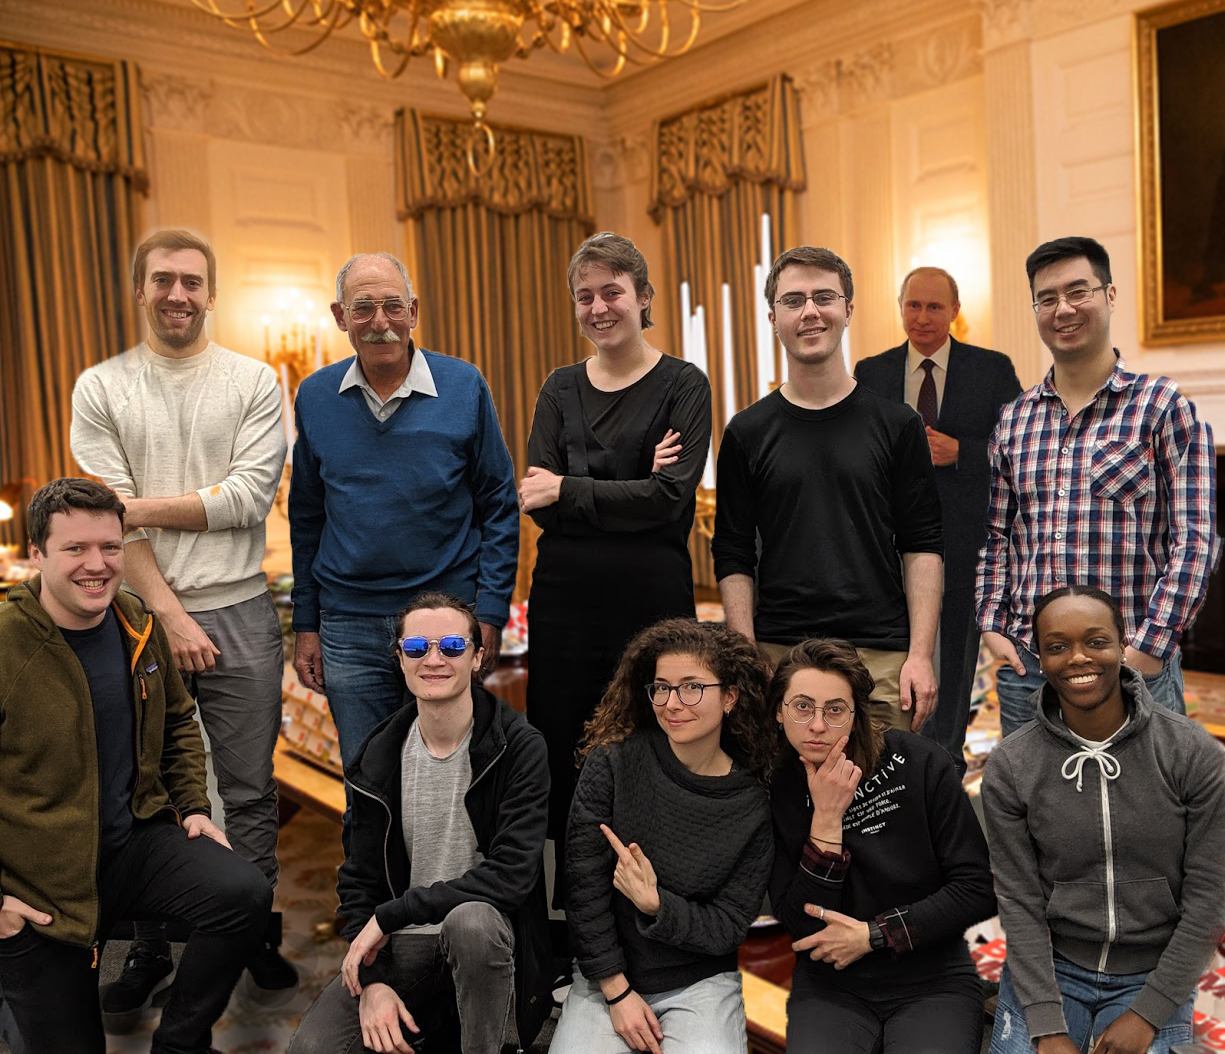
\includegraphics[width=\textwidth]{img/1/viral.jpg}
% \end{marginfigure}

% To Ethan, for sustained support and gentle provocation, and for leading me in all kinds of interesting directions, and towards all kinds of new knowlege.

% 
To Shannon, for all of your kindness, and for introducing me to the work of both Kevin Lynch and Mierle Ukeles, without whom I would be a lesser person (and this thesis would be terribly, terribly dull). Such a great exception to the idea that one should never meet their heroes!

% To Deb, for a phenomenal amount of support in almost everything I tried to do over the past 2 years, for help navigating the bureaucratic nightmare that is MIT’s accounts system, and for all the care you put into the group, and into the Lab.

% To the MAS staff -- Linda, Amanda, Monica, Keira and Lily in particular -- for all of the help, support and guidance.

% To all of the people who supported and took part in this project from around MIT, in particular Brian Goldberg and Ruth Davis, whose knowledge and enthusiasm for waste management made me know this project would be worthwhile.

% To everyone at the MIT Game Lab, who gave me tonnes of help and wisdom while I was developing this game. (and to \emph{everyone} who helped playtest, and took part in the studies)

% To Ray, for invaluable help with React, and to Robert, for Nginx witchcraft

% To MIT’s Living Labs Initiative, who generously funded this project.

% To The Viral Communications group: Kalli, Britney, Nchinda, David, Oceane, Sam, Mike, Veronika, Robert and other friends, for 2 years of friendship, support, and laughter. It’s been such a pleasure to work together all this time. Also big thanks to Kalli and Oc\'eane for helping me with waste audits while I was away from the lab.

% \begin{marginfigure}
% 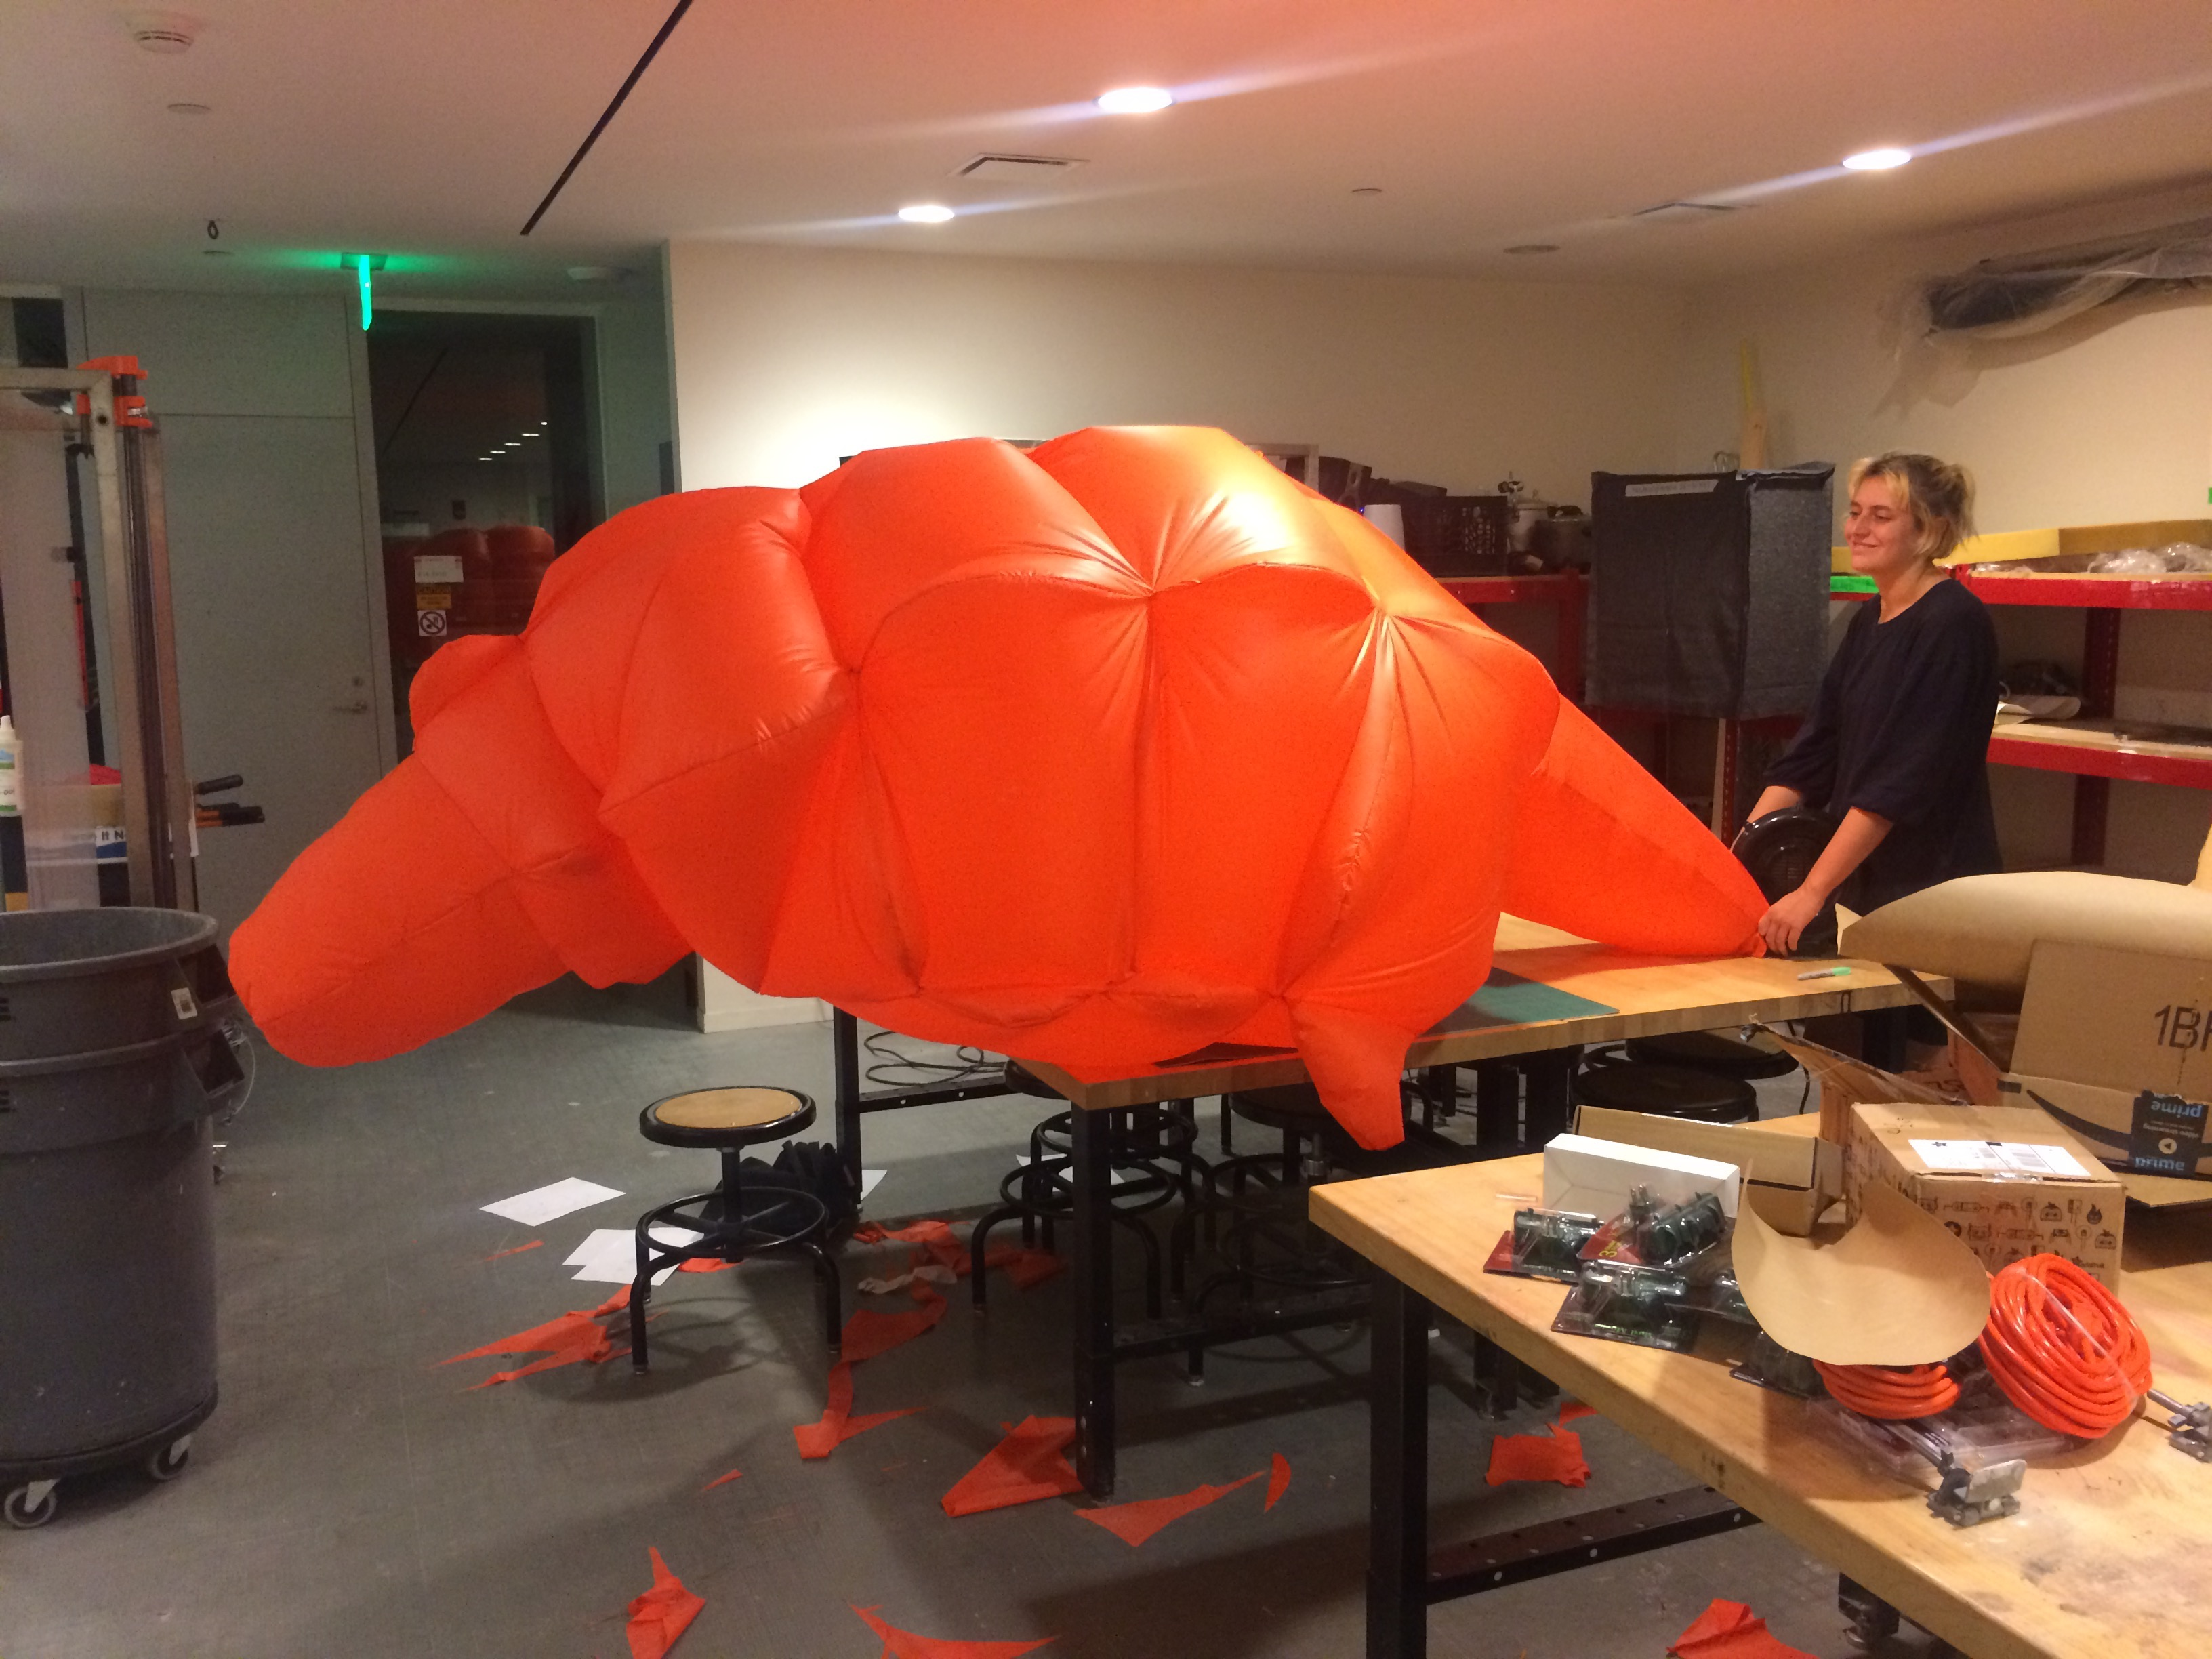
\includegraphics[width=\textwidth]{img/1/bugs.jpg}
% \end{marginfigure}

% To Travis, Hisham, Tomer and Ariel, serene group mothers, for unending wisdom, kindness, support, advice and optimism.

% To Tom, John and Graham, for teaching me how all the machines work \sidenote{read: letting me make memes on the embroidery machine}, and to Jay and Darrell, for teaching me how to make pots, skills I will take with me everywhere.

% To Sam and Rachel, and all of CAMIT, for funding our weird art.

% To everyone at the lab — far too many to list here, but Jake, Sara, Adam, Avery, Hane, Michiel, Pip, Oscar, Vik, Susan, Tom\'as, Miriam, Daniel, Alexei and Pedro for a start — who I hope to call friends for a very long time!

% To the Learning Initiative (particularly Katherine and Philip), for a wonderful festival of learning, and the opportunity to make many blobs.

% \begin{marginfigure}
% 
\includegraphics[width=\textwidth]{img/1/99f.png}
% \end{marginfigure}

% To Don, Dan, Spencer, Brian, Jifei, Sultan, David and Philip, for throwing bigggg parties (and letting me throw some too!)

% To Devora, truly a graduate woman of excellence.

% To Kalli again, for teaching me so much, about everything (but in particular: font choices, collaboration, critique, the internet and friendship).

% To the ACT programme, for being a warm and welcoming second home at the Institute, in particular to Kevin, Marion, Tobias, Nida and Azra.

% To Mike, and the rest of the staff at the Muddy Charles Pub (defacto third home), where around 70\% of this thesis was written, for cheap beer and a wonderful community.

% To my family — mum, dad, Irene, Albert — for all their support, and for instilling in me from a young age a love of art, a healthy suspicion of capitalism, and a ruthless approach to editing writing. I hope I can repay these efforts by becoming less employable with every passing year.

% \begin{marginfigure}
% 
\includegraphics[width=\textwidth]{img/1/terataki.jpg}
% \end{marginfigure}

% To Adam and Zach, esteemed residents of the Egg House, for making our home truly such a joyful and wondrous place to be. May there always be soup rounds in the freezer.

% To Terataki the axolotl, who has always had such an encouraging expression.

% To Market Basket, the closest I'll ever come to Heaven on Earth.

% Lastly, to Gary. I love you!!!


\newpage

\chapter*{Abstract}

If Waste is Information, what can be learned from an understanding of waste management at MIT as a complex information system? Through engaging people with their role within a waste system, can relations to and practices of waste management change? 

This thesis presents a framework for making and evaluating context-driven and critical civic games in partnership with local organisations. Working with waste management and sustainability efforts on campus, MIT is used as a living lab to study the link between interaction and action on `wicked problems'. More generally, this project looks at ways in which participatory, critical and exploratory games can give people agency over the complex systems that surround them. 

% \listoffigures
\tableofcontents


\newpage
\setcounter{page}{1}
\renewcommand{\thepage}{\arabic{page}}

\chapter*{Introduction}
\addcontentsline{toc}{chapter}{Introduction}

\begin{flushright}
% \begin{minipage}[b]{0.8\textwidth}
\begin{flushright}
\emph{After the revolution, who`s going
 to pick up the garbage on Monday morning?} \cite{ukeles_manifesto_1969}\\
Mierle Landman Ukeles
\end{flushright}
% \end{minipage}
\end{flushright}


\begin{flushright}
\emph{``A defining characteristic of the 21st century is mass reliance on technologies and systems that we know are important but understand little about''} \cite{onuoha_i_2016}\\
Mimi Onuoha
\end{flushright}

\begin{marginfigure}
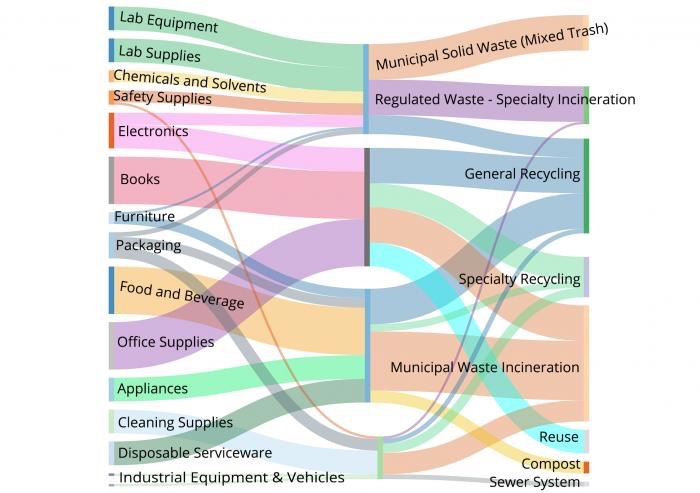
\includegraphics[width=\textwidth]{img/2/perlman-material.jpg}
\caption{A diagram by MITOS Fellow Rachel Perlman, showing material flows on campus}
\end{marginfigure}

Waste is an issue that manifests at both global and local scales. Within the US, landfill capacity is predicted to decrease by around 2.6\% year-on-year, and around 5\% in the Northeast \cite{waste_business_journal_waste_2017}. The recycling rate for Municipal Solid Waste is around 34\% (around a third of that is currently exported), with the remaining portions relegated to landfill (80\%) and incineration (20\%) \cite{epa_advancing_2018}. The past year has seen major stresses on the worldwide recycling infrastructure, as China (previously one of the world's largest processors of recycling) has stopped accepting several kinds of recyclables \cite{albeck-ripka_your_2018}, and has decreased the required contamination rate for materials to be accepted to far below the previous norms \cite{germin_chinas_2018}, forcing many American cities to incinerate their contaminated municipal recycling for lack of another option \cite{milman_moment_2019, albeck-ripka_your_2018}. In areas where recycling rates have historically been high, this shift in framing from recycling as a social good, to a commodity subject to a shifting economic landscape (and increasingly destined for landfill) has left residents feeling angry, frustrated and disempowered \cite{albeck-ripka_your_2018}.

MIT as an institute is a part of this waste system. MIT produces approximately 5500 tonnes of waste annually, of which around 31\% goes on to be processed as single-stream recycling. For Casella, the Mixed Recycling Facility (MRF) that sorts MIT's recycling, the changing economic landscape means that they can no longer accept recycling that is contaminated with non-recyclables, as the purity required by China is so much higher \cite{casella_2018_2018}. Achieving the newly-stringent contamination rate has been a challenge, both for MIT, with multiple trucks of recycling turned away from Casella in the past few months, and fines for contamination levied.

%elucidate: casella struggling so has also become much stricter with institutions
5 years ago, MIT's Office of Sustainability (MITOS) was formed to improve the Institute's waste lifecycle, with a focus on diverting waste from landfill, reducing recycling contamination, and addressing how goods are consumed across campus. The waste that MIT produces (and the qualities thereof) is necessarily a product of both an environment and a population.

%wicked problems and representational crises

This thesis is not about `smart' waste technologies, but about how people might come to terms with waste (and `waste well') when these technologies are insufficient. How people decide to take action on civic issues is a matter of little consensus, relating in part to the attention and care we afford to these issues. This thesis explores the civic game as a means of directing this attention in a way that is playful, exploratory, and critical, and engendering care in a system for which people care very little. In particular, it examines how we might use games to make civic systems legible and visible, and how that legibility and visibility can lead to action. It uses the local population of MIT as a study, but it presents an approach and a set of tools that seek to be generalised.


\begin{marginfigure}
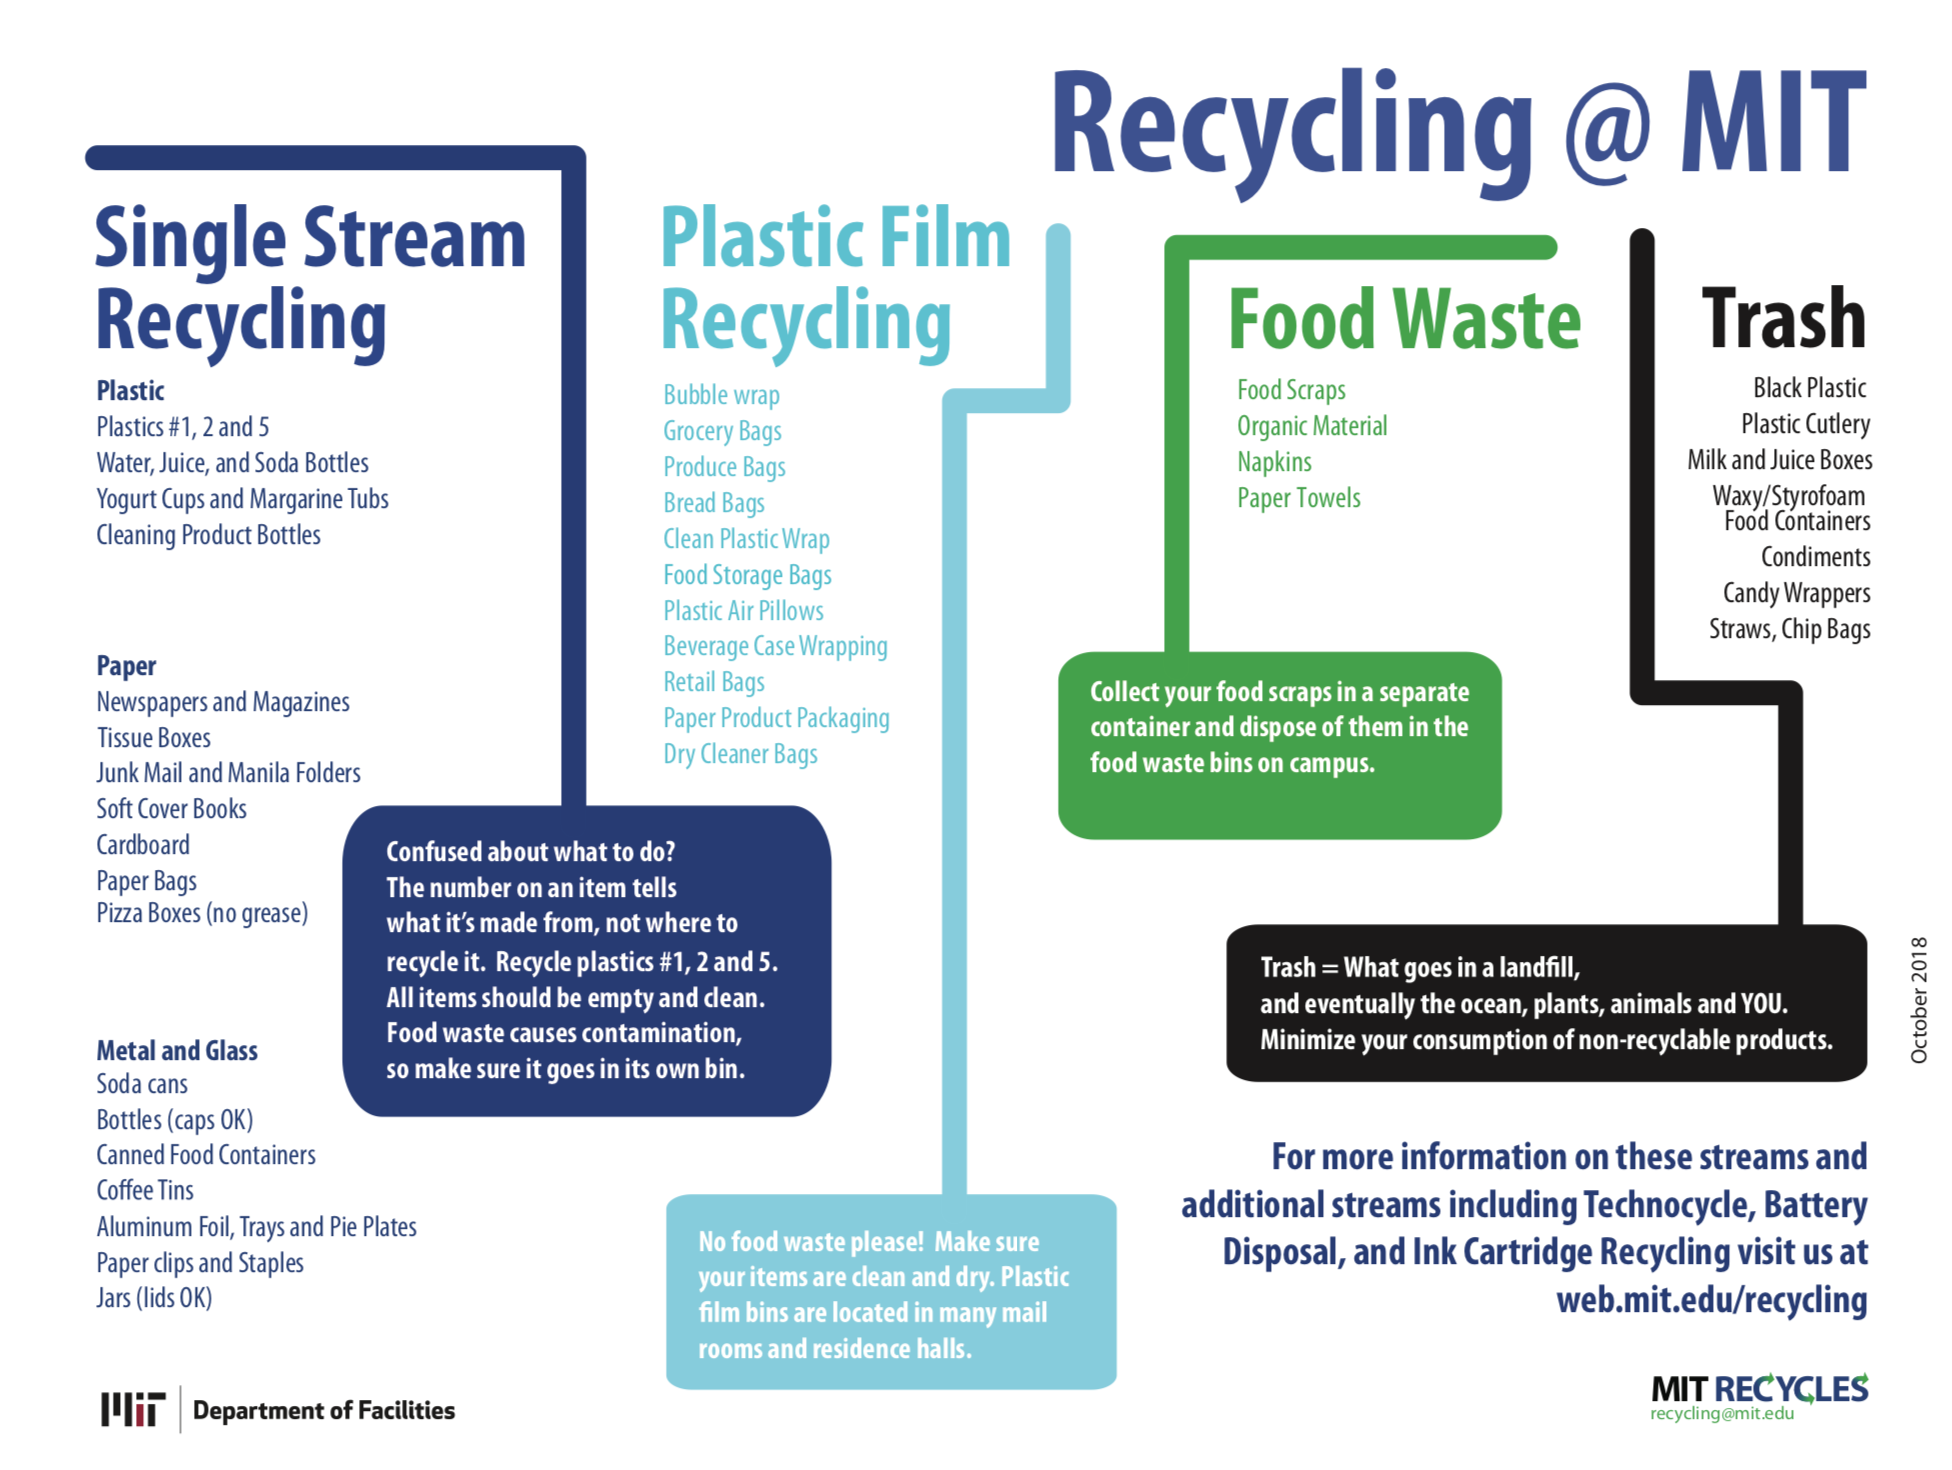
\includegraphics[width=\textwidth]{img/1/flowchart.png}
\caption{A guide to waste disposal by MIT Recycles}
\end{marginfigure}

\subsection*{Outline}

In \emph{Designing With(in) Public Organisations}, Andr\'e Schamin\'ee outlines a framework for collaboration between designers and the public sector. His focus is centered on design as a means of addressing `wicked problems'\cite{rittel_dilemmas_1973} through collective co-operation, and much of the book is centered on the role designers can play in broadening the scope of public intervention. In the diagram below, Schamin\'ee outlines stages of progress in such collaborations: first by understanding the problems at stake (in particular, finding a `paradox' inherent in current approaches to tackling the problem at hand), by empathising with the actors in the system, by `re-framing' the problem, and by proposing a solution. \cite{schaminee_designing_2018}

\begin{figure}
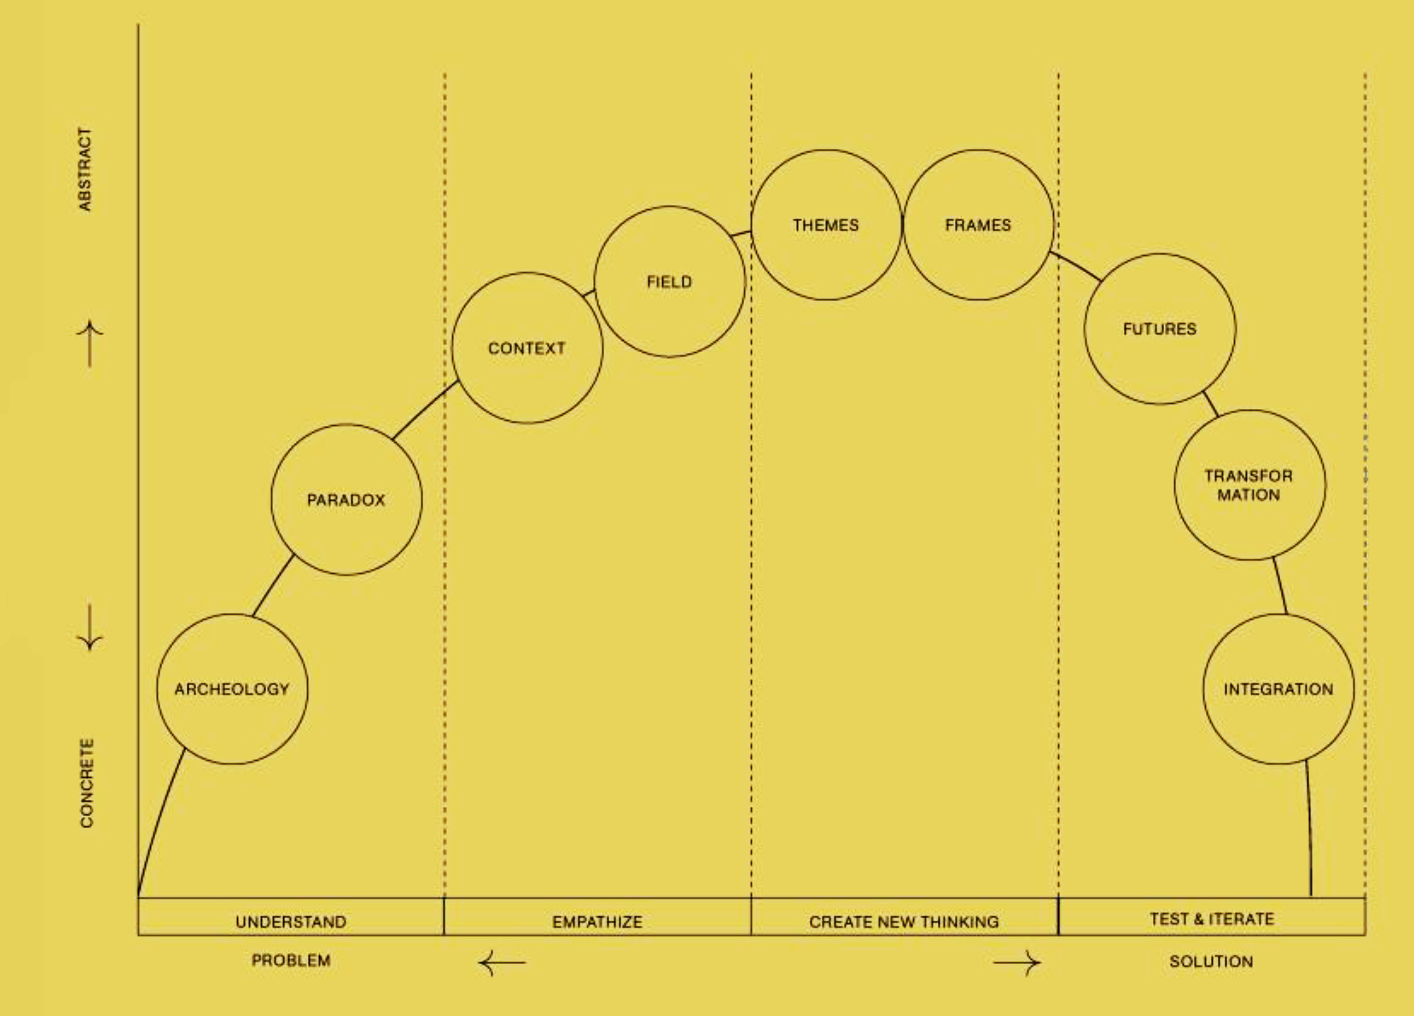
\includegraphics[width=\textwidth]{img/1/design-stages}
\caption{Schamin\'ee's stages of design with public organisations \cite{schaminee_designing_2018}}
\end{figure}

The stucture of this thesis broadly follows this arc, and is organised into 4 parts. The first comprises a contextual and methodological background, exploring questions of legibility and representation in waste, and forms of participation and intervention in complex civic systems. In the second, I introduce the Media Lab's Zero Waste Pilot Programme, toward which this project contributes, and discuss the results of field research. In the third, I identify key themes from part two, and describe the development of two `civic games' aimed at addressing these. In the fourth section, I outline two studies that examine the effectiveness of these games, and analyse their results.

\chapter{Representing Waste}

\begin{flushright}
\emph{Treating waste as information means following the heterogeneous network of connections in which a piece of garbage is embedded.} \cite{offenhuber_waste_2017}
Dietmar Offenhuber
\end{flushright}

\begin{flushright}
\emph{Nobody wonders where, each day, they carry their load of refuse. Outside the city, surely; but each year the city expands, and the street cleaners have to fall farther back.}\cite{calvino_invisible_1974}\\
Italo Calvino, Invisible Cities
\end{flushright}


In \emph{Archives of the Present-Future: On Climate Change and Representational Breakdown}, Emily Scott uses the phrase `representational breakdown' to describe the inherent contradictions in representing global problems in a way that can elicit a proportionate response. Her thesis is that the current visual imaginary of climate change relies on `single picture[s]': in failing to adequately represrent the complex role of humans in this system, we are rendered `desensitised and deactivated' spectators, rather than agents capable of action.

Our cultural imaginary of waste is similarly lacking. Urbanist Kevin Lynch writes that, when confronted with waste, ``we avoid the subject, acting like those who chose their eyes and scream when most in danger''. In his book \emph{Waste is Information}, Dietmar Offenhuber makes central the notion that ``infrastructure governance is enacted through the representations of the infrastructural system''. In other words: the way a system is represented plays a large role in shaping our understanding of it, and thus shapes our behaviour within it. Here, his characterisation of waste as `information' refers to the ``traces of many social, cultural, technical, and political processes'' that can be `read' from a waste system, and from its representations \cite{offenhuber_waste_2017}. 

In this chapter, I take representation as a point of departure to examine the context of civic legibility, attention, participation and behaviour. I give a short historical account of problems specific to waste systems, but attempt to draw conclusions that have general relevance to other civic systems that suffer from the same crisis of representation.

%other representationally difficult systems
%internet, energy, democracy?
%emily scott: climate change and representational breakdown

\subsection*{When smart is not enough}

\begin{flushright}
% \begin{minipage}[b]{0.8\textwidth}
\begin{flushright}
\emph{``It is important to understand that diversion from disposal is not recycling. Collection is not recycling. A product is not recycled until it is made into another product.''}\cite{morawski_understanding_2009}\\
Claire Morawski, Container Recycling Association
\end{flushright}
% \end{minipage}[b]{0.8\textwidth}
\end{flushright}

\begin{marginfigure}
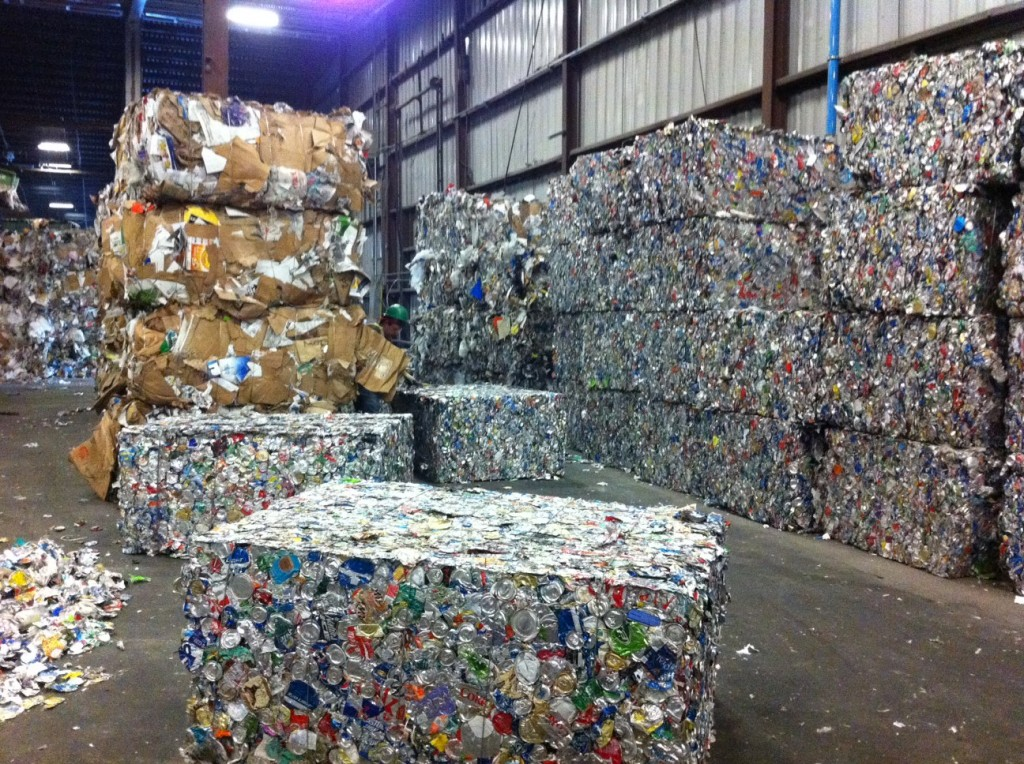
\includegraphics[width=\textwidth]{img/1/casella-bales.jpg}

\vspace{1cm}

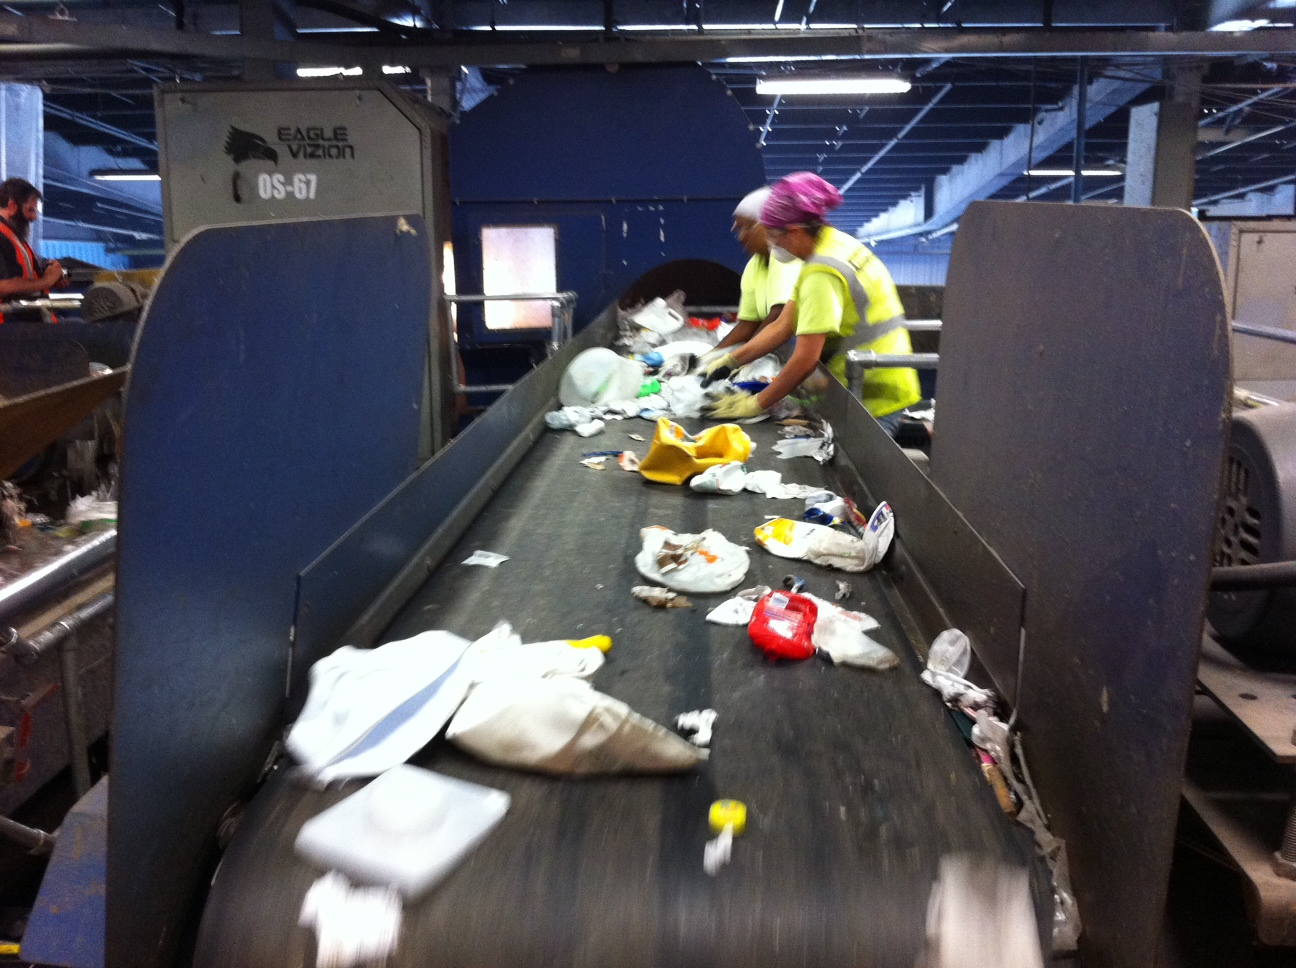
\includegraphics[width=\textwidth]{img/1/casella-sorting.jpg}
\caption{Baled recycling and manual sorting in Casella's Mixed Recycling Facility \cite{delichatsios_trash_2011}}
\end{marginfigure}

Single stream recycling was developed in California in the 1990s, and has since become the dominant form of recycling in the United States \cite{laskow_single-stream_2014}. Initially lauded for increasing the rates of collection of recyclable materials, and decreasing the load on curbside collection rounds, the efficacy of single-stream as a means of preserving resources is not as clear. Single-stream recycling allows all recycling to be placed in the same container, processed together at a Mixed Recycling Facility (MRF) by a combination of machinery and human sorting. However, while MRFs make it possible to sort multiple waste streams from one another, for many materials the eventual quality of the reclaimed product is significantly lower than if they had been processed separately \cite{morawski_understanding_2009}. During the growth of single-stream recycling, this was less of a problem: countries such as China were prepared to buy and process lower-quality baled stock, making this an economically viable option for processing large quantities of recycling. However, China's ``National Sword'' program has significantly reduced the market for some forms of poor-quality recycling (in particular plastics), leading to a large proportion of recycling in the United States going to landfill or incineration, and throwing the efficacy of single-stream into question \cite{milman_moment_2019, albeck-ripka_your_2018, martin_reverberations_2017}.

\begin{marginfigure}
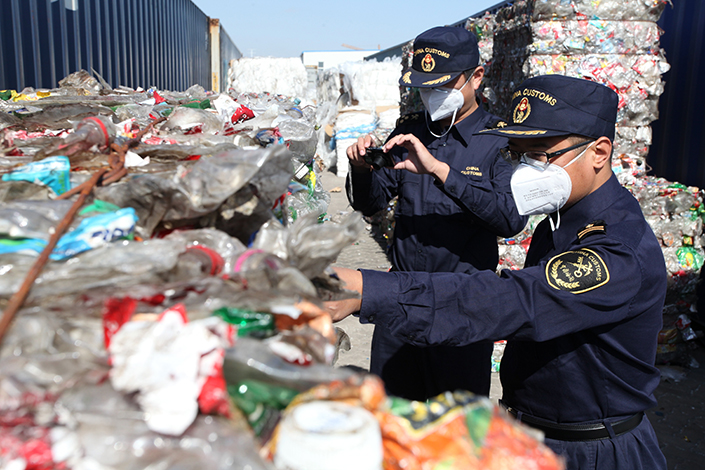
\includegraphics[width=\textwidth]{img/1/china-recycling-inspection.jpg}
\caption{Chinese customs officials assess the quality of bales of recycled plastic \cite{martin_reverberations_2017}}
\end{marginfigure}

Ultimately, the convenience and apparent seamlessness of single-stream recycling belies the constant upkeep required to maintain it. The process of sorting recycling must still take place, and almost always involves human sorting labour as a component of the `high-tech' separation process. As Mattern remarks on the `smart' waste chutes installed at the Hudson Yards development: ``they cultivate an out-of-sight, out-of-mind public consciousness... garbage becomes more of a domestic aesthetic problem than an ecological concern.'' She asks instead whether the designers might provide a view of Swedish company Envac's ``smart, efficient'' waste collection system, making legible the infrastructure of disposal. \cite{mattern_instrumental_2016}

\begin{marginfigure}

\includegraphics[width=\textwidth]{img/1/casella-plastic-bag.png}
\caption{A recycling worker removes plastic bags jamming a sorting machine in a Casella recycling plant. \cite{casella_recycle_2018}}
\end{marginfigure}

This is not to say, of course, that it is not important to build technologies that deal with our waste as cleanly and efficiently as possible (particularly for the sake of people working with them). However, a distinction between efficiency (in an energetic sense) and convenience is necessary: friction, such as needing to sort recycling or walk further to a bin can be a positive force. This is not a concept unique to waste systems: for example, in the current context of fake news and social media overuse, the concept of a `good friction' (and variants thereof) are often cited as ways by which we might negotiate a healthier relationship with the internet \cite{donath_signals_2011, tufekci_twitter_2017}. In her book \emph{Friction: An Ethnography of Global Connections}, Anna Tsing sees what she terms the ``zone of awkward engagement", and ``the sticky materiality of practical encounters" as essential for action on complex global problems. \cite{tsing_friction_2005}. %ADDSENT good friction: who are good refs?

There is a tendency in infrastructural systems to obscure the `hard parts': be they human labour, piles of trash, server farms or fibre-optic cables \cite{mattern_infrastructural_2013}. We make custodial workers come in late at night, export our waste to where we can't see it, and bury the mounds of cable, silicon and glass that we use to support our `connected' lives underground. Not only is the direct effect on the affected communities and ecosystems (those without the option to hide the real effects of these infrastructures) harmful \cite{liboiron_why_2014}, but in making these processes `like magic' we also remove a sense of collective responsibility for them.

\begin{marginfigure}
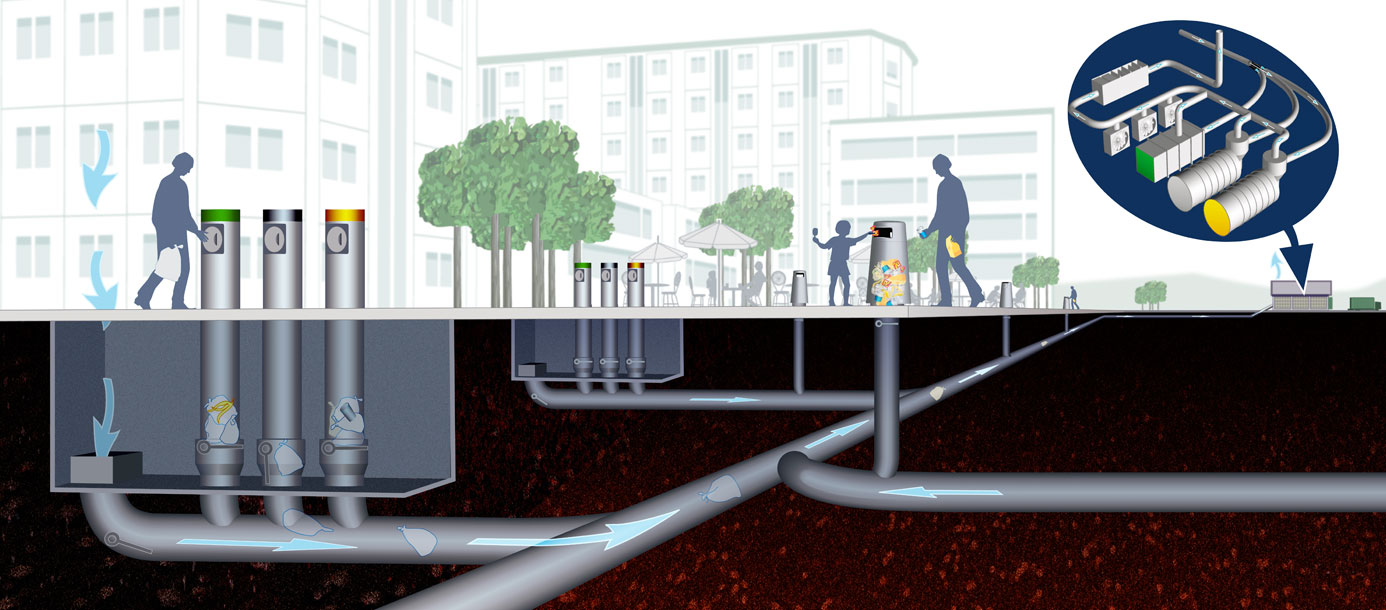
\includegraphics[width=\textwidth]{img/1/envac.jpg}
\caption{``Bins, but not as you know them'' -- a graphic from Envac's website, showing subterranean waste chutes \cite{envac_smart_nodate}}
\end{marginfigure}

%wendy chun?
\subsection*{Seeing Waste}

\begin{flushright}
\begin{minipage}[b]{0.8\textwidth}
\begin{flushright}
\emph{``If people were not quite so horrified by trash, so convinced that, 
once tossed out, it should by all rights disappear, they might be able to 
control litter better. Paying attention is the first step.''} \cite{lynch_wasting_1990} \\
Kevin Lynch
\end{flushright}
\end{minipage}
\end{flushright}

In \emph{Wasting Away}\cite{lynch_wasting_1990}, Kevin Lynch writes extensively on how we see waste, asking what it might mean to `waste well' -- to be at peace with our relationship with waste, and deal with it thoughtfully and rationally \sidenote{\emph{Wasting Away} was Lynch's last book, and never fully completed: it was published 6 years after his death in 1984 with the help of the editor Michael Southworth.}. In a similar manner to his more famous work \emph{The Image of the City} (in which he studies the mental models that we construct of urban spaces) \cite{lynch_image_1960}, so Lynch writes at length on the disparity between our imagination of waste systems, and their actual operation. He argues that wasting is a cultural construct, one overloaded with emotion and anxiety, thus making its related habits hard to shift.

\begin{marginfigure}
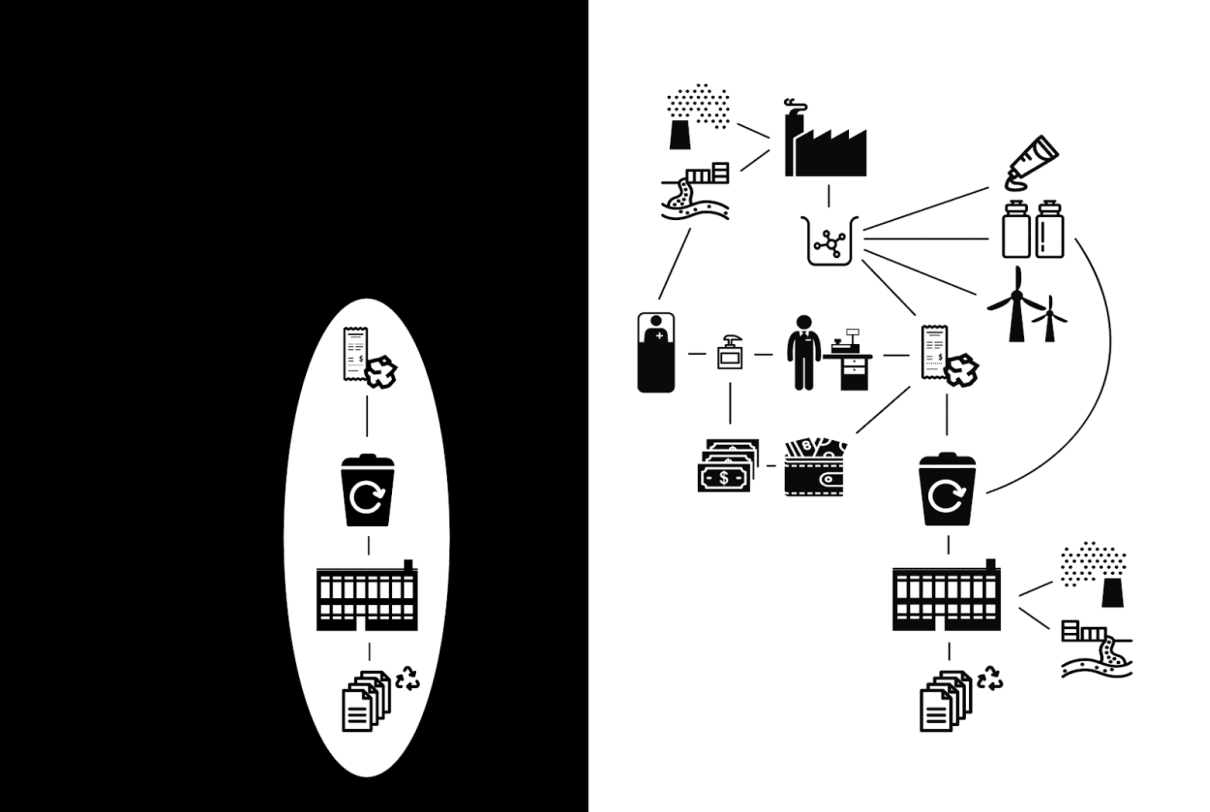
\includegraphics[width=\textwidth]{img/1/waste-complexity.png}
\caption{Comparing an image of the waste system to its manifestation. \cite{liboiron_why_2014}}
\end{marginfigure}

%%IMAGE TO ADD: emotive recycling campaign
% can it live somewhere else?
% \begin{marginfigure}
% 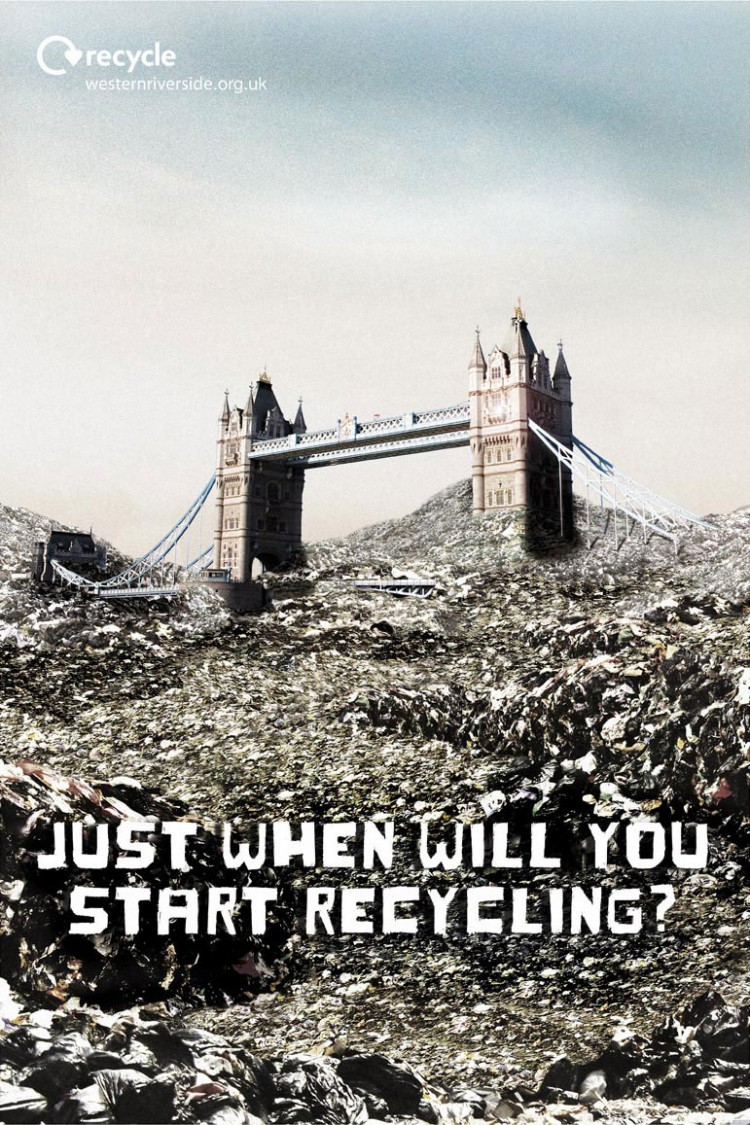
\includegraphics[width=\textwidth]{img/1/recycling-riverside.jpg}
% \caption{Adverts by the Recycle Western Riverside authority. \cite{noauthor_recycle_2006}}
% \end{marginfigure}

Max Liboiron argues that our imagination of waste is necessarily limited to a small component of a much larger system: one that encompasses not just our empirical experience of wasting (e.g. disposal, compost and recycling) but also a much broader range of social, economic and environmental effects \cite{liboiron_why_2014, liboiron_mapping_2014}. Liboiron also decries the common representation of waste as a behavioural problem, arguing that given that industrial waste comprises a far greater proportion of global waste streams than municipal waste, it is structural rather than social change that is needed \cite{liboiron_against_2014}. In reference to overly-emotive recycling campaigns, Gay Hawkins remarks that ``Our imaginations are overflowing with the horror of waste'', a horror that is as paralysing as it is counter-productive \cite{hawkins_ethics_2006}.

Lynch reminds us that, no matter how we may wish it, there is no such thing as throwing `away' \cite{lynch_wasting_1990}. Wastes endure -- for someone, somewhere -- and as the world's population concentrates ever more in large cities, this fact becomes more apparent.

\subsection*{Maintenance Art}

\begin{flushright}
\emph{Who should handle all your dirty jobs? Someone else! Someone else! Someone Else!} \cite{reardon_trash_1998}\\
Homer Simpson, ``Trash of the Titans``
\end{flushright}

\begin{marginfigure}

\includegraphics[width=\textwidth]{img/1/simpson-truck.png}
\caption{Homer Simpson, newly-elected head of Springfield's Waste Management services, rides elated atop a garbage truck \cite{reardon_trash_1998} }
\end{marginfigure}

Maintenance art gives us a means to look not only at waste, but also those tasked with its disposal, and associated forms of work: garbage collection, street cleaning, sanitation work, sorting recycling. The term originates from Mierle Ukeles'  `manifesto for maintenance art 1969'\cite{ukeles_manifesto_1969}, a feminist critique of what she calls the `avant-garde death instinct' of technological progress, in which she re-figures the work of cleaning and repair as an artwork in itself. Ukeles uses the museum as a vehicle to confront people with waste and the people who handle it: for her piece `Touch Sanitation Performance' (made as the artist in residence at the New York department of Sanitation), she spent a year shaking the hand of each of the 8,500 New York Sanitation workers who would accept the offer.\cite{ukeles_touch_1980}

\begin{marginfigure}
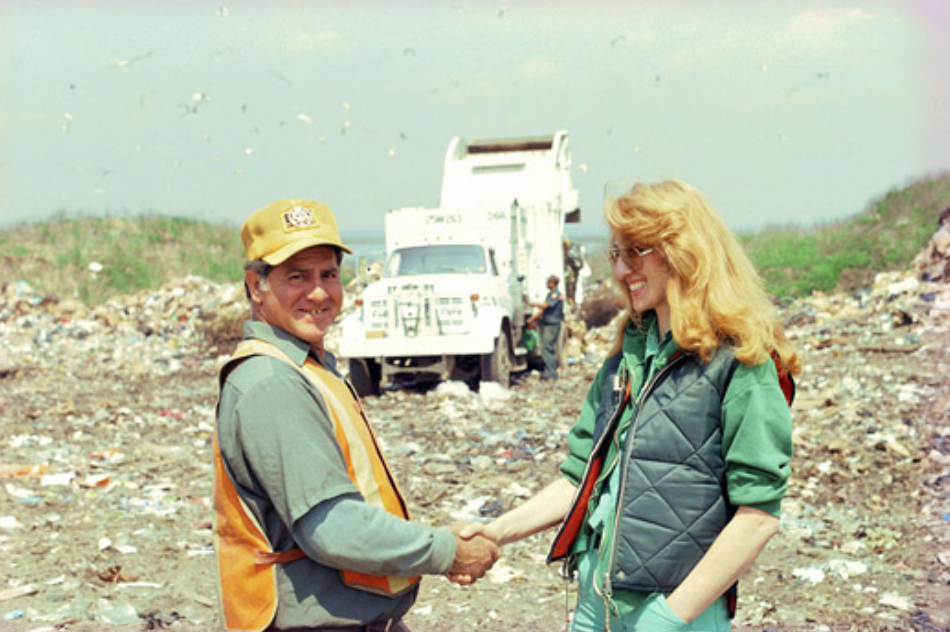
\includegraphics[width=\textwidth]{img/1/touch-sanitation.png}
\caption{A shot from \emph{Touch Sanitation Performance}, 1980 (via Ronald Feldman Gallery, NY)}
\end{marginfigure}

More contemporary examples of maintenance art include Jenny Odell's Bureau of Suspended Objects --  the result of a residency program at the San Francisco dump -- where she attempted to trace the provenance of 100 objects she found on the site, presenting them in a museum, accompanied by their histories, in the manner of archeological relics \cite{odell_archive_2015}. Weina Lin's Disassembly Line takes the contemporary work of deconstructing e-waste (a form of labour commonly exported by the United States) within a gallery, inviting viewers to bring objects for a team of assistants to strip down and recycle \cite{lin_disassembly_2016}.

\begin{marginfigure}
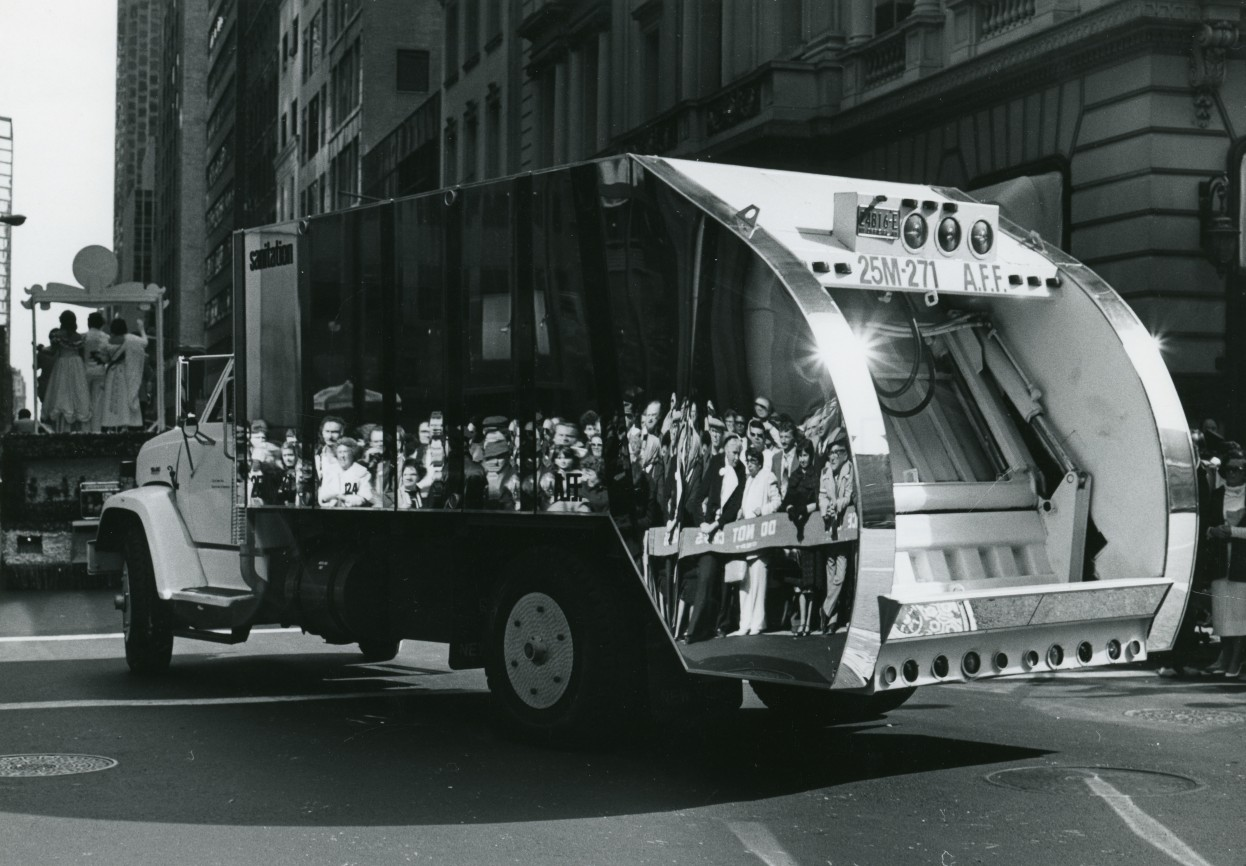
\includegraphics[width=\textwidth]{img/1/social-mirror.jpg}
\caption{Ukeles' \emph{Social Mirror}, 1983 (via Ronald Feldman Gallery, NY)}
\end{marginfigure}

Maintenance art forces the viewer to confront realities that are abject, guilt-inducing and uncomfortable as beautiful and engaging in their own right. Ukeles' description of  Freshkills landfill site as a huge `social sculpture' challenges our norms of how waste should be seen\cite{cotter_artist_2017}. These works also underlie an important point: by properly taking care of waste: be it breaking down cardboard boxes, separating recycling, taking care to remove plastic bags and contaminants, you are considerate toward those who would handle it next.

\subsection*{Infrastructure legibility}

\begin{flushright}
\emph{What does it mean for mapping that a hallmark of modern waste is invisibility?}
\cite{liboiron_mapping_2014}\\
Max Liboiron
\end{flushright}

%%IMAGE TO ADD: sim city
\begin{marginfigure}
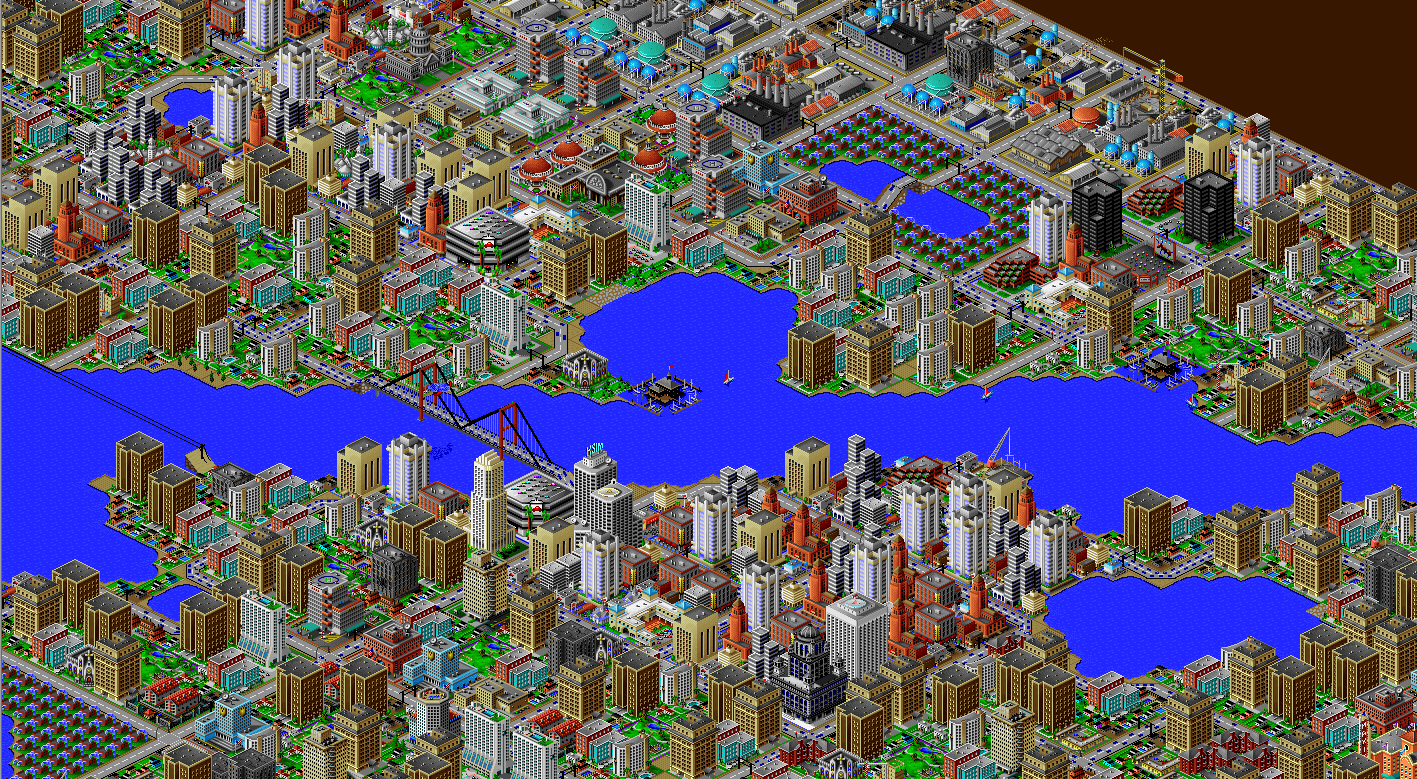
\includegraphics[width=\textwidth]{img/1/sim-city.png}
\caption{A still from Sim City 2000}
\end{marginfigure}

The term infrastructure legibility was coined by Dietmar Offenhuber in his book \emph{Waste Is Information}, to refer to the problem of representing civic infrastructures too complex to be understood in their entirety \cite{offenhuber_waste_2017}. This is an idea that draws heavily from Lynch, who defines the ``legibility'' of a system as ``the ease with which its parts can be recognised and can be organised into a coherent pattern''. 

%make this a bit more nuanced >> a pattern language refss

There is, of course, a tension between creating a legible representation, and over-simplifying a narrative. Representations can inherently encode the assumptions or biases of the author: for example, Ava Kofman notes that the `advice' in SimCity 4's manual coerces a particular political viewpoint \cite{kofman_les_2014}. As one player put it in an interview with Los Angeles Times in 1992 ``I became a total Republican playing this game. All I wanted was for my city to grow, grow, grow.''\cite{Baker_model_2019}

Bret Victor's essay \emph{Explorable Explanations} goes some way towards addressing these issues: by providing people with tools to interrogate the assumptions behind a particular representation, Victor proposes that one might draw a more nuanced conclusion. Instead of seeing a particular piece of information as ``right or wrong'', ``bad or good'','' a representation becomes ``one point in a large space of possibilities.'' Victor terms this `active reading', transforming a text from something to be read, to ``an environment to think in'' \cite{victor_explorable_2011}. While often watered down to the somewhat overused phrase `systems thinking', the assertion that a systemic representation has different affordances to texts and images is central to popular framings of waste in terms of `Lifecycle Management' and the `Circular Economy'.

%%IMAGE TO ADD:a brighter idea
\begin{marginfigure}
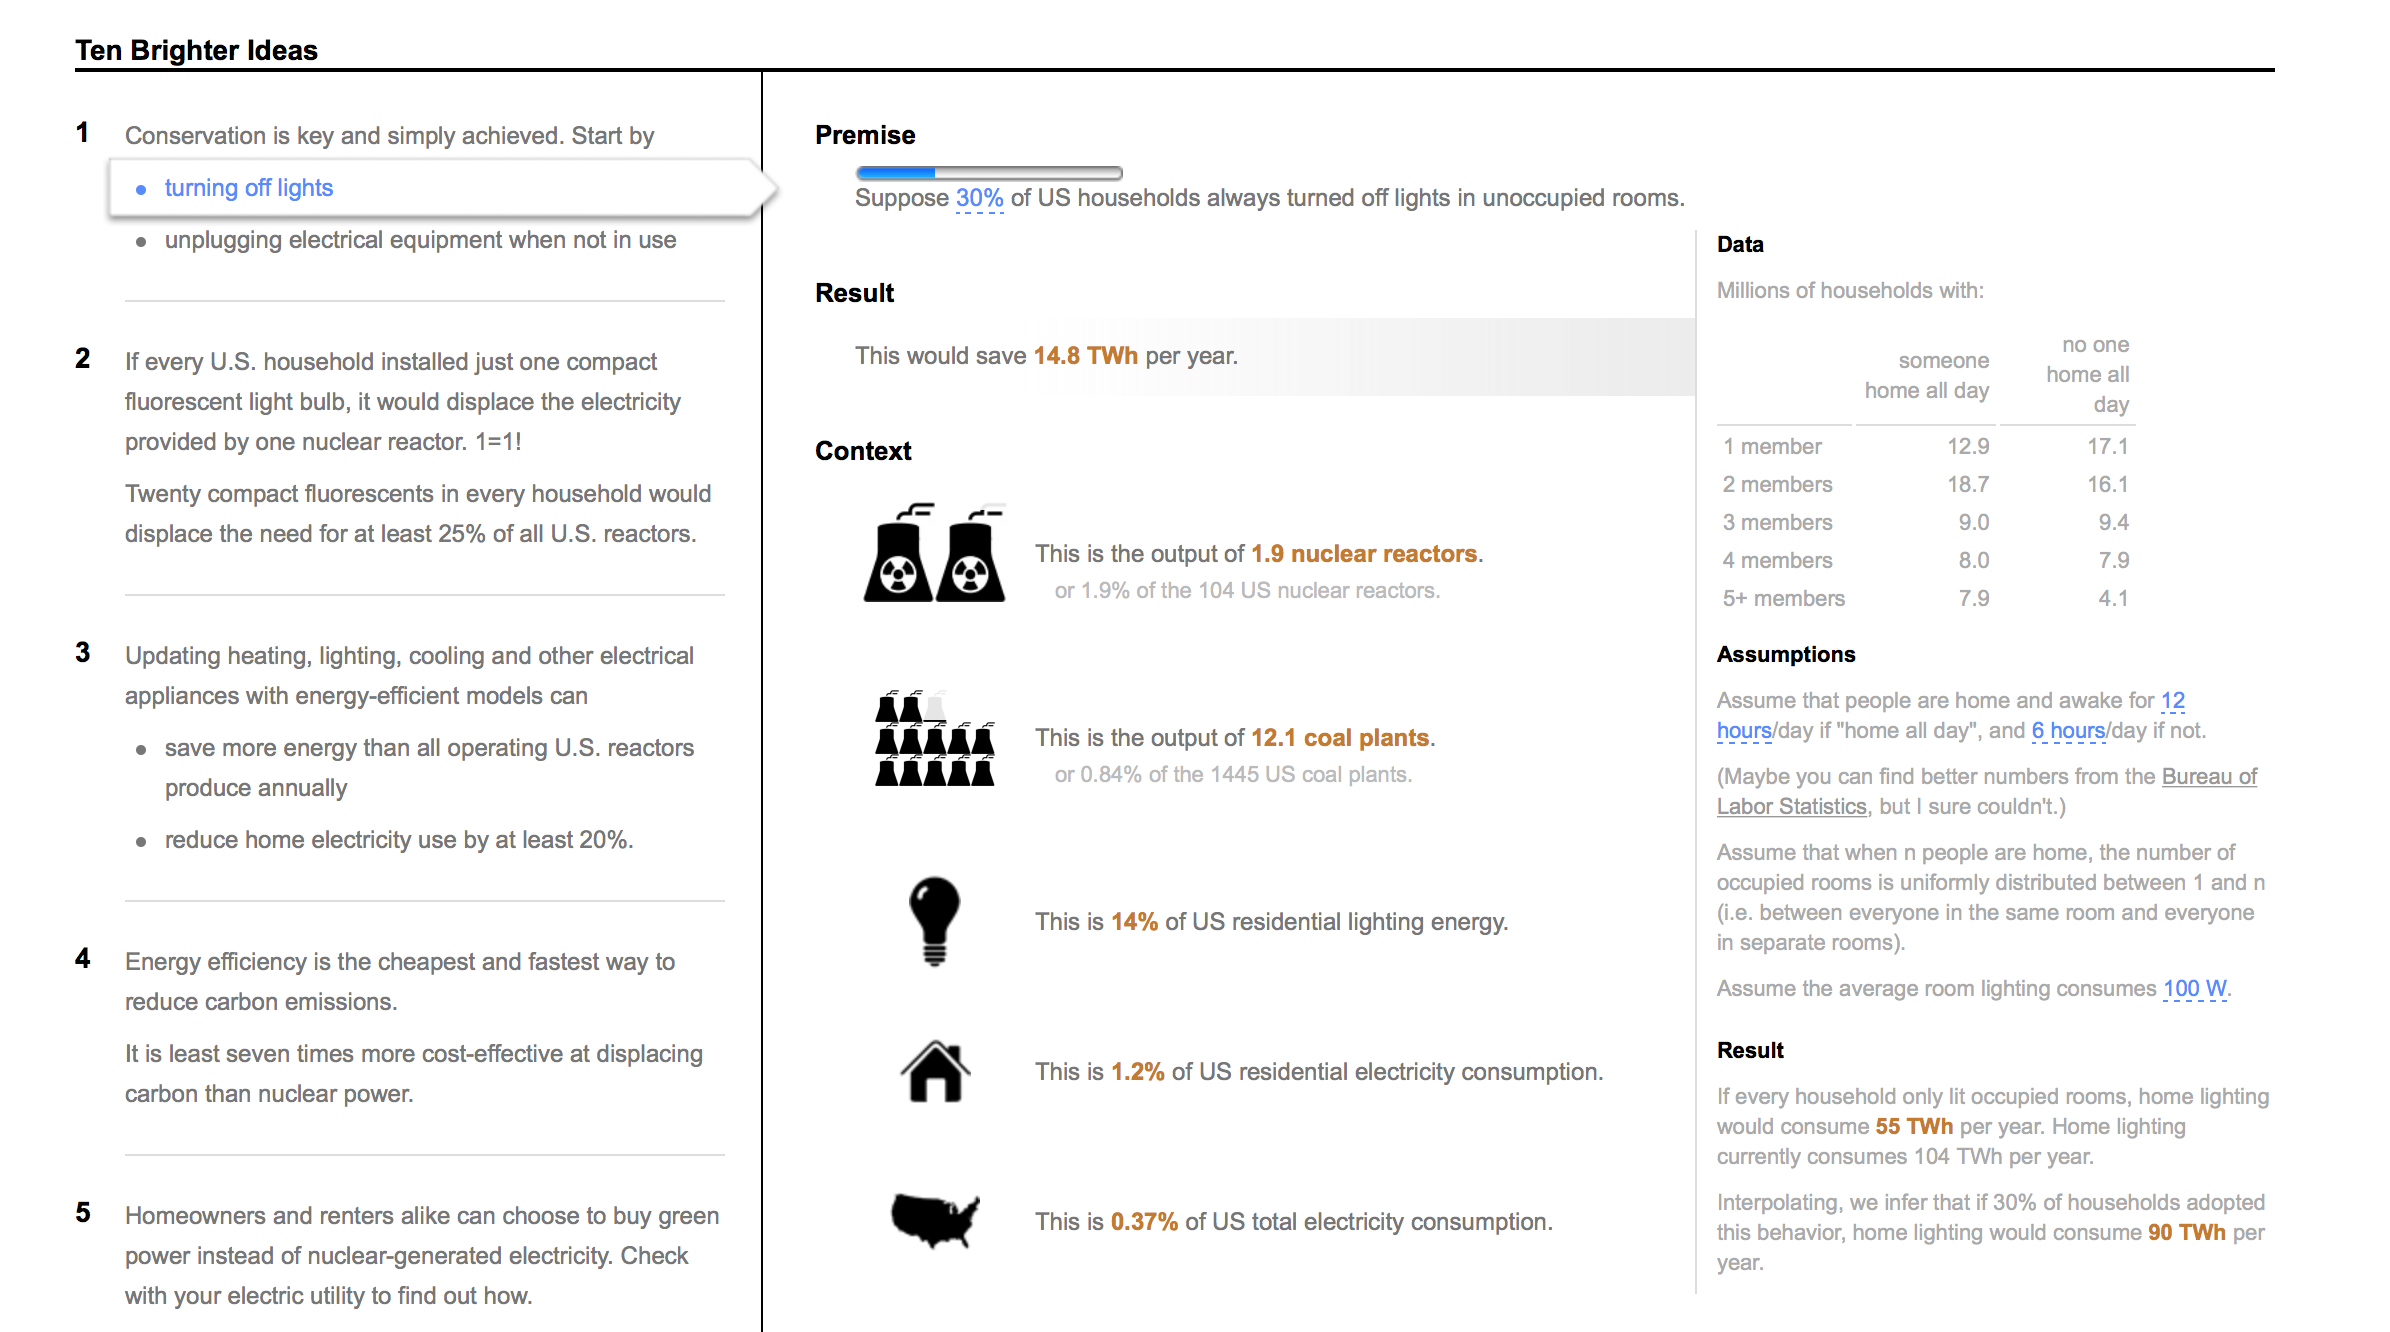
\includegraphics[width=\textwidth]{img/1/ten-brighter-ideas.png}
\caption{A still from Bret Victor's \emph{Ten Brighter Ideas?}, an `explorable explanation' of climate policy \cite{victor_ten_2010} }
\end{marginfigure}

\subsection*{Systems Dynamics}

\begin{flushright}
\emph{Systems happen all at once} \cite{meadows_thinking_2008}
-- Donella Meadows
\end{flushright}
%%add in here: wicked problems, dilemmas in a general theory of planning
The figuring of urban infrastructures as information systems dates back to the 1960s, where Jay Forrester (who had founded the field of Systems Dynamics a decade before) worked with former mayor of Boston John F. Collins, to produce the book \emph{Urban Dynamics}\sidenote{Incidentally, along with fellow cyberneticist Christopher Alexander's \emph{A Pattern Language}, it is this text that formed the main foundation for Sim City's game mechanics \cite{kofman_les_2014}}. A key thesis of Forrester's is that, in considering cities, organisations or even countries as feedback systems, one can glean powerful and counter-intuitive insights as to the root causes of particular problems. %add some critique here?

\begin{figure}
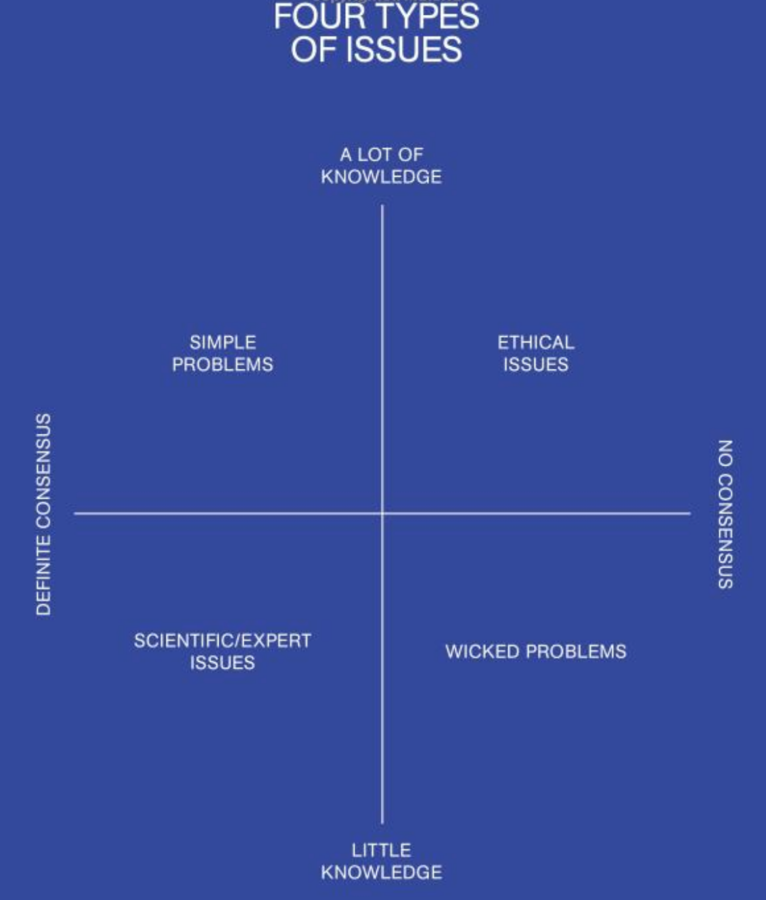
\includegraphics[width=\textwidth]{img/1/problem-types.png}
\caption{Andr\'e Schamin\'ee's taxonomy of `issue types' in working with public organisations, identifying wicked problems as an intersection of low information and low consensus. \cite{schaminee_designing_2018}}
\end{figure}


Horst Rittel and Melvin Webber's influential paper `Dilemmas in a General Theory of Planning' \cite{rittel_dilemmas_1973} applies systems ideas to coin the term `wicked problem', describing numerous social policy problems whose complexity defies a traditional solutionist approach. Waste -- as an infrastructure characterised by poor representation, and a lack of social and political consensus as to how to deal with it -- is an example of such a problem \cite{liboiron_trash_2012}. 
\begin{marginfigure}
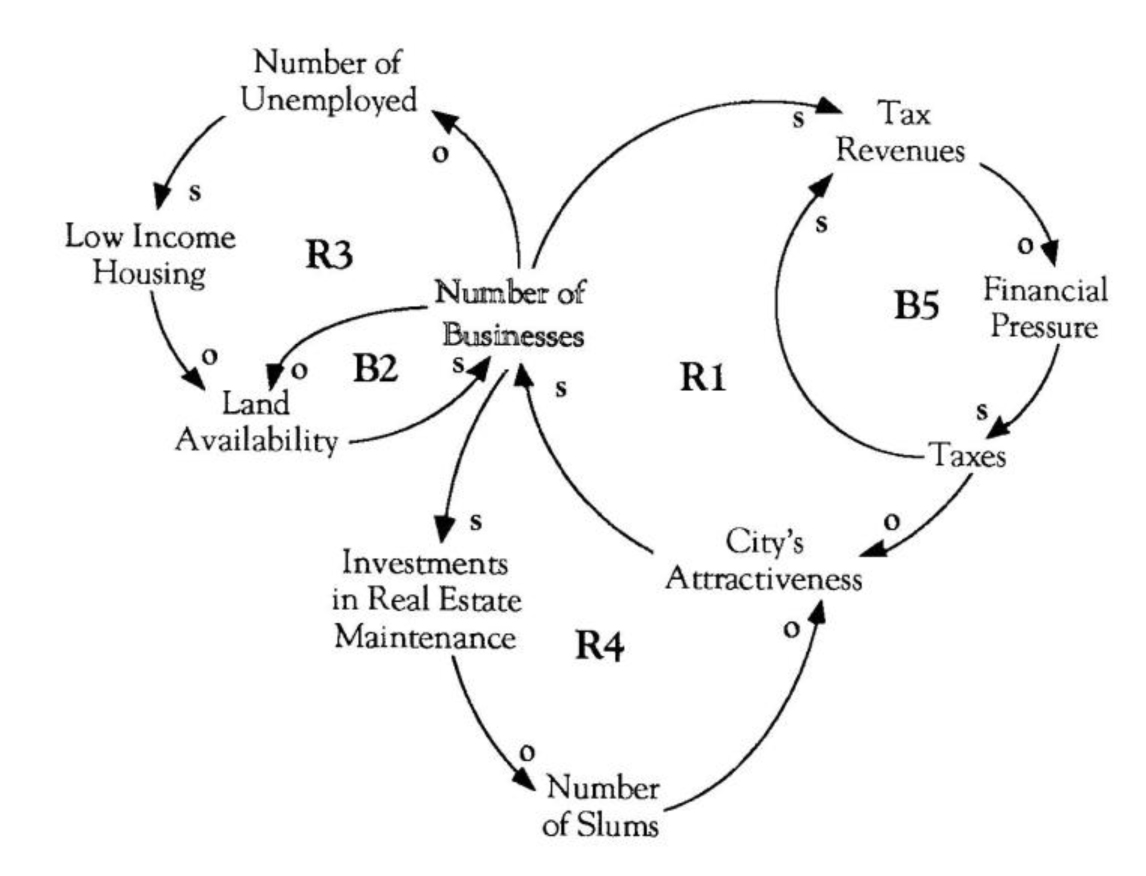
\includegraphics[width=\textwidth]{img/1/urban-dynamics.jpg}
\caption{A feedback diagram from Forrester's \emph{Urban Dynamics} \cite{forrester_urban_1969} }
\end{marginfigure}
Rittel and Webber argue that `scientific' systems methods `of the first order' are inadequate for dealing with social problems, asserting that `one cannot first understand, and then solve'. The `second-order' approach they advocate for considers a social system to be one of a system of systems, of which the modeller themselves is also a part. Second-order social systems simulation techniques such as agent-based modelling remain popular as models of collective behavior, and have been used to model urban phenomena including segregation \cite{schelling_dynamic_1971}, resource acquisition \cite{epstein_growing_1996-1}, and gentrification \cite{batty_new_2013}. The use of these models in urban planning is not without controversy: a common criticism is that the information they impart is highly abstracted, and can encode the biases of the modeller: it is one thing to use simulations to understand a dynamic in an urban system, and another to use them build cities anew.

\begin{marginfigure}
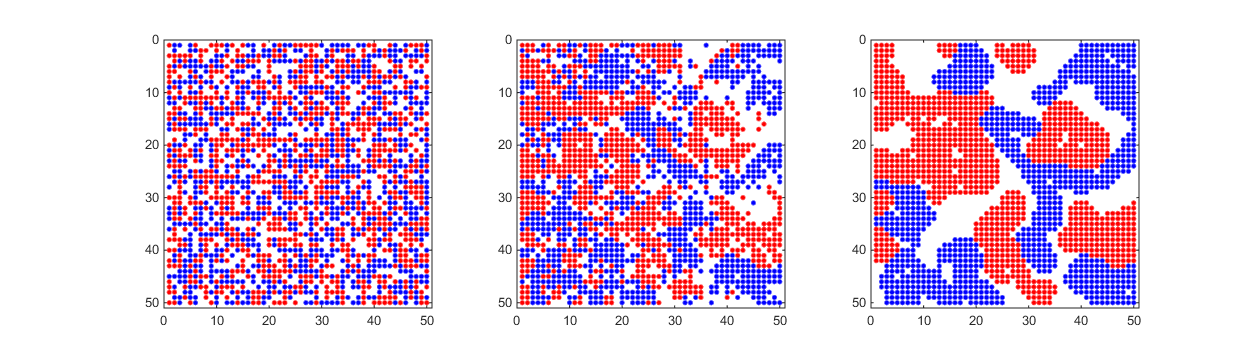
\includegraphics[width=\textwidth]{img/1/schelling-segregation.png}
\caption{An implementation of Thomas Schelling's agent-based segregation model, showing the simulation's progression \cite{schelling_dynamic_1971} }
\end{marginfigure}

\begin{flushright}
\emph{``All models are wrong, but some are useful''}
-- George Box
\end{flushright}

%contemporary urban simulation, simulation more generally
%\subsection*{Why Simulate?}

\begin{marginfigure}
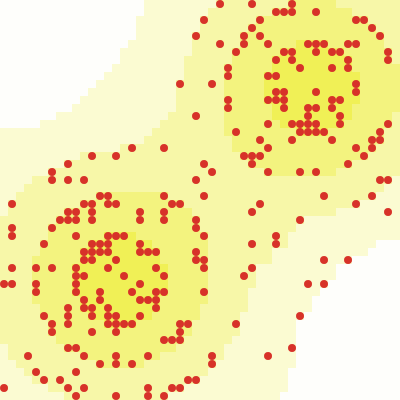
\includegraphics[width=\textwidth]{img/1/sugarscape.png}
\caption{An image of the \emph{`sugarscape'} simulation -- part of Epstein and Axtell's \emph{Growing Artificial Societies} \cite{epstein_growing_1996-1}}
\end{marginfigure}

In `Leverage Points: Places to Intervene in a System', Donella Meadows enumerates the effectiveness of 12 different `sites of intervention' in a system, noting that often (particularly in public, political and civic systems), it is the least effective forms of intervention (numbers and constants) that receive the greatest deal of attention \cite{meadows_leverage_1997}. Meadows also emphasises the effectiveness of the information feedback loop, citing a study where a group of houses with a electricity meter installed by the door used 30\% less energy than an identical group where the meter was in the basement. Perhaps, if we took our refuse to the dump daily, or spent time regularly with the workers who clean our office buildings by night, we might have a different attitude to our waste. Lynch certainly thinks so, opining for a time where ``Wasting things could be as valued and interesting as making and consuming them''. %add something something attention something

In this analysis, however it is important to acknowledge that the greatest changes to be made are often structural. Just as Max Liboiron points out, in her essay `Against Awareness, for Scale: Garbage is Infrastructure Not Behaviour', the agency of the individual in the system is limited by the goals, politics and dynamics of waste systems themselves. In the U.S., where around 98\% of waste is industrial (rather than municipal)\cite{liboiron_against_2014}, and it can use more energy to rinse a glass bottle in order to recycle it than it does to throw it away \cite{tierney_reign_2018}, it would be irresponsible to advocate for any change of behaviour without acknowledging the broader infrastructure at work.

\subsection*{Waste as a complex system}

\begin{flushright}
\emph{``Where there is dirt there is system``} \cite{douglas_purity_1966}\\
Mary Douglas 
\end{flushright}

Equally, however, it would be defeatist (and inaccurate) to insist that one has no leverage over waste systems. Liboiron argues that `even if individual actions don't save the world, they are expressions of an ethic that can lead to other actions that do scale.'\cite{liboiron_against_2014}

An example of a scaling action is that of recycling contamination. Recycling contamination is a huge contemporary issue, as it not only results in a high volume of otherwise good recycling diverted to landfill, but, if not caught, a single contaminated bag can cause an entire truck to be turned away at the recycling plant, a costly and wasteful error. Further down the line, China (a key importer of recycling) will reject any received shipment deemed to be greater than 0.5\% impure \cite{casella_recycle_2018}; ships containing contaminated loads turn back around, and head to landfill. \cite{albeck-ripka_your_2018}. Tackling contamination requires action at the level of the individual, both in showing more care when disposing of waste (to avoid obvious contaminants such as food waste), and in maintaining awareness of what can and cannot be recycled. Livia Albeck-Ripka of the New York Times identifies the second set of behaviours as `aspirational recycling' \cite{albeck-ripka_6_2018}: wanting to believe that objects can be recycled (such as coffee cups, greasy boxes, food-filled containers) that are in reality contaminants. The source of this cognitive dissonance is in part the cultural association with recycling as a fundamentally `good' action, rather than a complex, energy-consuming set of economic and industrial processes \cite{tierney_reign_2018}.

%IMAGE TO ADD: common contaminants
\begin{marginfigure}
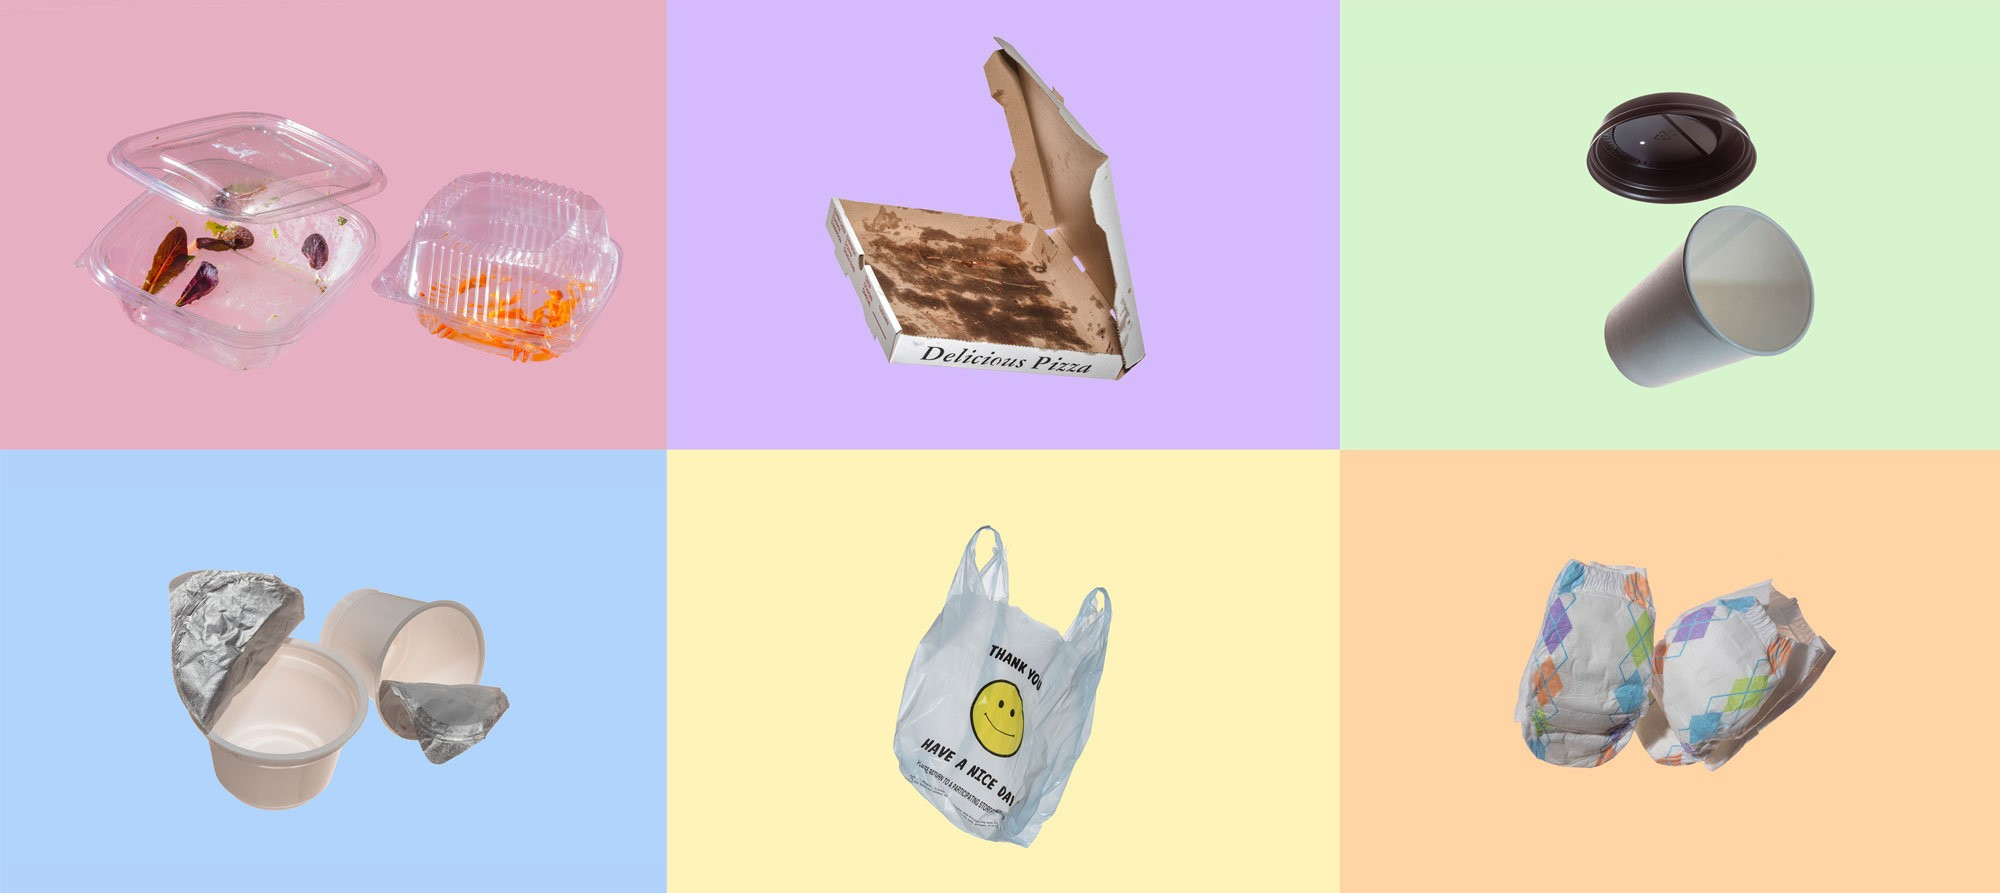
\includegraphics[width=\textwidth]{img/1/contaminants.jpg}
\caption{Common recycling contaminants \cite{albeck-ripka_6_2018}}
\end{marginfigure}

It is through taking such a systems perspective on waste that we might participate more effectively. It is unfortunate that `recycling well' often involves not recycling at all: but if we can accept that recycling is a poor substitute for not consuming in the first place, we are provided with an alternative. In designing interventions to a waste system, it is also worth considering what it is about the system that we want to change. Even if recycling well does not make a huge amount of difference to the environment, it might make a much more immediate difference to the people who handle our waste directly \cite{liboiron_against_2014}.

\section*{Changing the Way We Waste}

\begin{flushright}
\emph{``A despised process, in which despised people handle despised material, seems out of control. Advanced technology will not solve it. The missing element is cooperation and care.''}\cite{lynch_wasting_1990}\\
Kevin Lynch
\end{flushright}

%more recycling history here,

Since around the 1970's (which marked the passing of the Resource Conservation and Recovery Act in the United States), the problem of municipal waste has been linked both to personal responsibility, and to an environmental cause. At present, the minimisation of municipal solid waste is broadly framed as a co-operative problem that we are all expected to play a role in solving. Interventions into waste streams can take place at the site of production (for example, minimising wastes created by industrial processes and logistics), the site of consumption (encouraging consumers to buy less, or reuse), and the site of disposal (recycle, compost). As has been observed by Liboiron \cite{liboiron_against_2014}, when it comes to civic education, focus tends toward changing habits of disposal, despite its relative ineffectiveness when compared to consumption, or changing the industrial context in the first place. The `waste hierarchy' model is often used to illustrate relative merits of different diversion strategies, distinguishing between Reduction, Reuse, Recycling and Recovery.

% and disposable packaging economic externalities

\begin{marginfigure}
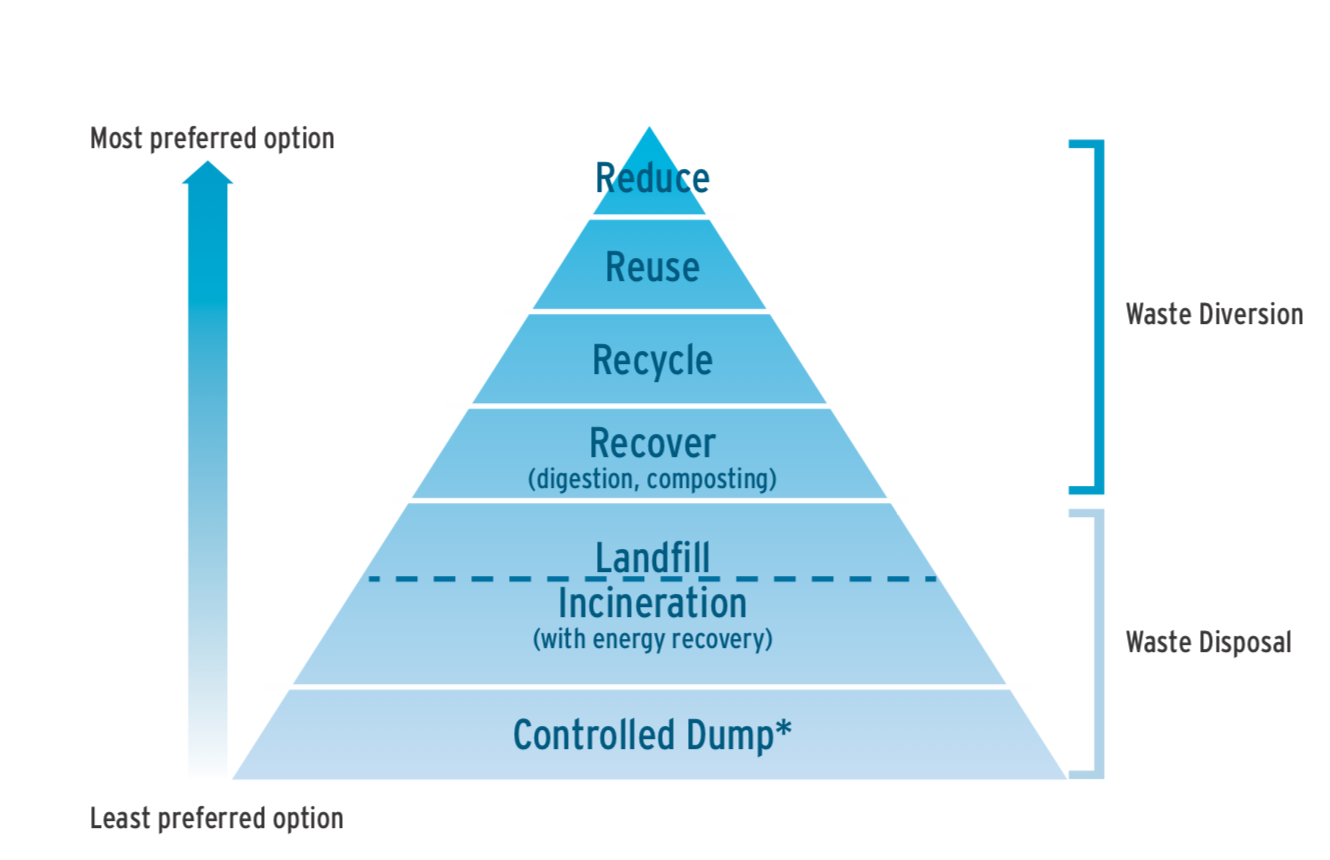
\includegraphics[width=\textwidth]{img/1/recycling-hierarchy.png}
\caption{A waste hierarchy diagram}
\end{marginfigure}

Offenhuber writes that ``Waste systems cannot be separated from systems of production, and notions of value cannot be seen in isolation.'', advocating for a `whole-systems' approach to waste infrastructure. In municipal waste systems, efforts to `change the way we waste' typically involve an infrastructural change, combined with some form of behaviour or attitudinal intervention on the part of the citizen, even if that change is unconscious or involuntary. For example, in Max Liboiron's description of her intervention in Columbia University, while it involved no `awareness' campaign whatsoever, use of plastic bottles was drastically reduced simply by removing their availability, and by providing for re-usable bottles; a shift in infrastructure leading to a change in habit. \cite{liboiron_against_2014}

In this section, I examine attitudes to change wasting behaviors on the scale of the individual, the building, and the municipality. Interventions of this sort necessarily bring together a number of different disciplines, including behavioural psychology, urbanism, design, and supply-chain management. Here, the focus is on municipal solid waste (rather than industrial waste, or other municipal streams such as waste-water), as this is the focus of this project.
%more specific

\subsection*{Waste, Attitudes and Behaviors}

\begin{flushright}
\emph{``Every participatory system needs to acknowledge this limitation: you cannot
 rely on the end goal being incentive enough to encourage individuals to 
participate and cooperate on achieving the end goal.''} \cite{haque_notes_2008}\\
Usman Haque
\end{flushright}

In \emph{Infrastructural Tourism}, Shannon Mattern explores a number of interventions seeking to `make legible' invisible civic infrastructures. Discussing a range of projects, including visualisations of communications satellites, DIY tours of California Interstates and sonified railway bridges, it is towards the end of the piece that she asks: ``So you know where your Internet lives ...now what?'' \cite{mattern_infrastructural_2013}. The impact of such interventions can be hard to quantify, with the projects she descibes evaluating their successes along diverse metrics of participation, perception and increased critical thinking. In \emph{Can We Measure Media Impact?} Schiffrin and Zuckerman offer a survey of metrics used by news organisations to assess the real-world change made by their work, highlighting the difficulty in understanding impact that falls between traditional measures such as `likes' or `shares' on a piece of digital journalism, and direct and demonstrable action taken because of it (``Did a law change? Did the bad guy go to jail? Were dangers revealed? Were lives saved?''). Characterising this middle-ground as an `open problem', they distinguish between reach (propagation of the story), influence (effects on personal attitudes and public dialog) and impact (driving policy change or social movement) as separable modes for measuring media impact. \cite{anya_schiffrin_can_2015}

When examining infrastructural interventions that concern the environment, the link between `influence' and `impact' -- attitudes and behaviors -- is subject to an range of complex social phenomena. Most of the research on the link between awareness, norms, attitudes and behaviours (both observed and self-reported) around Environmentally Responsible Behaviours (ERBs) such as recycling can be split between intervention-based research (where particular interventions in a system are compared for their effectiveness) and determinants-based research (which examines emotional, attitudinal, behavioural and demographic factors). Meta-analyses such as Varotto and Spagnolli \cite{varotto_psychological_2017}, and Huffman et. al \cite{huffman_when_2014} make links between these modes of analysis.

% nicer link between this and previos para
Many studies of ERBs (and specifically those relating to recycling) use the Theory of Planned Behaviour (TPB) to theorise the link an individual's attitudes and their resultant behaviours. TPB is a prominent \emph{reasoned action} model used to predict an individual's intention to engage in a behavior within a specific context, which proposes that intention to perform a behaviour is driven by 3 determinants: attitudes towards a behavior, subjective norms, and percieved behavioral control, and that the intention to perform the behaviour, combined with percieved control, are the factors that subsequently determine the actual behaviour. \cite{ajzen_theory_1991}. Other models applied to explain recycling behaviours include Value-Belief-Norm theory (VBN, discussed below) \cite{huffman_when_2014}, the Theory of Reasoned Action (TRA, a forerunner to TPB), and the Theory of Normative Conduct.

\begin{marginfigure}
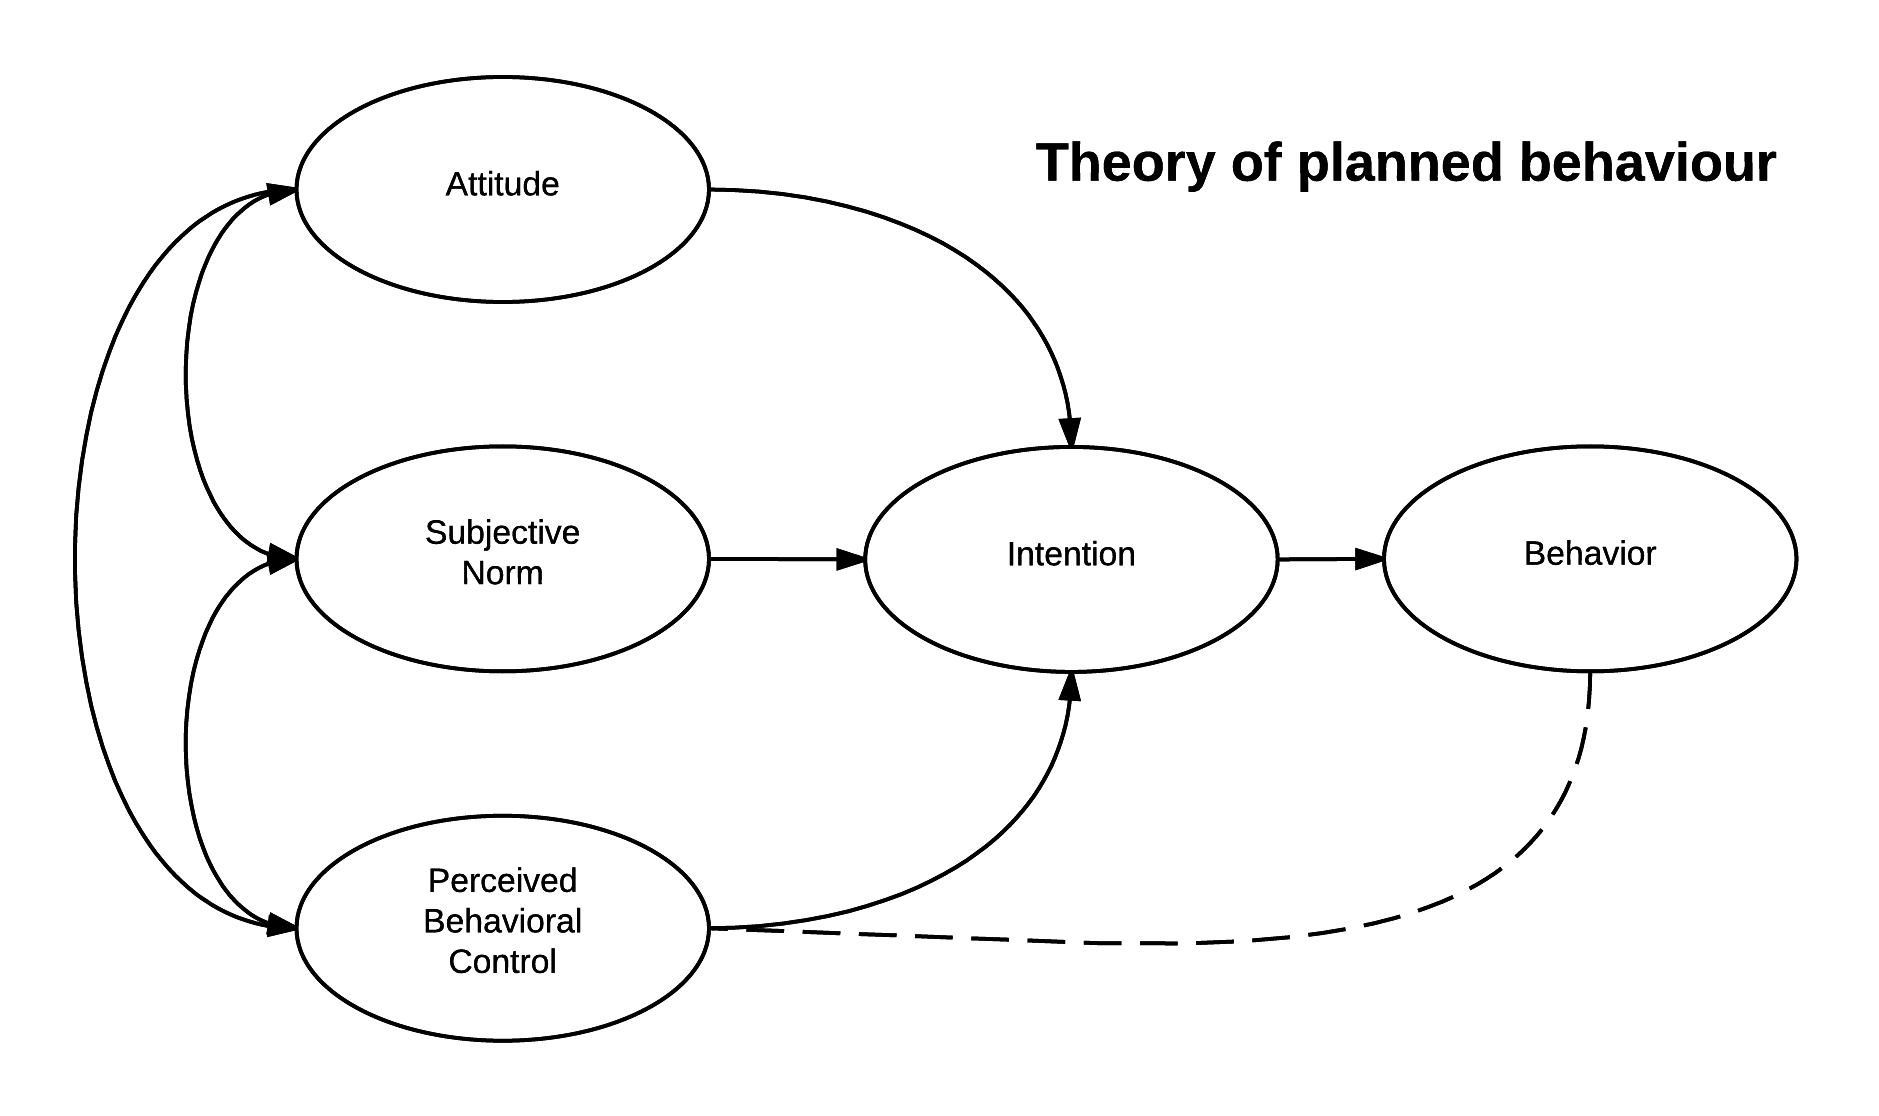
\includegraphics[width=\textwidth]{img/1/tpb.png}
\caption{The Theory of Planned Behaviour \cite{ajzen_theory_1991}}
\end{marginfigure}

%here describe attitudes and subjective norms
Percieved behavioural control (PBC) relates to the individual's perception of how easy or difficult it is for them to perform a behaviour, if they wish to. This originates from the theory of self-efficacy, which descibes an individual's belief in their innate ability to achieve goals \cite{bandura_self-efficacy_1982}. An internal efficacy is the notion that one understands a system and can participate in it, whereas an external efficacy is control over the system itself. However, a lack of external efficacy does not necessarily preclude effective participation in a system: much as political campaigners (for the most part) do not possess any great power to make governments respond to their demands, they can still be effective as individuals with high internal efficacy \cite{zuckerman_mobilizing_2019}.
%%make this better!!

Huffman et. al propose a 5-point scale for understanding the nuances of an individual's percieved agency when performing ERBs, drawing on Self-Determination Theory, which suggests that the greater the autonomy an individual thinks they have when making a decision, the better the long-term behavioural outcomes related to that decision \cite{huffman_when_2014}. This is borne out in much broader behavioural economics, with numerous studies finding that when rewards are offered for performing particular behaviours, the behaviour does not persist when the reward is removed.

\begin{figure}
\includegraphics[width=\textwidth]{img/1/internal-external.png}
\caption{Scale of self-determination in relation to recyling behaviours \cite{huffman_when_2014}}
\end{figure}

% Environmental psychology is a field of social psychology that examines the relationship between people and their surroundings, `including built, social, natural and virtual environments, the use and abuse of nature and natural resources, and sustainability-related behavior. \cite{noauthor_journal_nodate}'

Within studies of behaviour and the environment, TPB may be used to explain the disconnect between the behavioural intentions of sustainable practices (e.g., actions such as recycling carry strong positive normative beliefs), and actual behaviours. Stern and Oskamp propose that environmental action is influenced by a combination of linked internal and external factors: the external being physical infrastructures, institutions, and economic forces, and internal being attitudes, information, education, beliefs and behaviours\cite{stern_managing_1987}. Guagnano et. al apply this model specifically to recycling practices, showing that recycling behaviours are only observed when both positive internal attitudes, and positive external conditions are present\cite{guagnano_influences_1995}.

Wilma Strydom applies TPB specifically to conduct a systems-assesment of potential social interventions around recycling, using large-scale surveys to construct a specific model of the TPB. Her analysis concludes that Percieved Behavioural Control has a much greater contribution to behavioural than even the intention to perform that behaviour (which itself is shaped mostly by social norms), in line with the findings of Stern and Oskamp, and Guagnano et. al. She concludes with the importance of both considering the particularities of each local context, and in co-designing interventions with residents to ensure that they feel in control of local waste infrastructure. \cite{strydom_applying_2018}

\begin{figure}
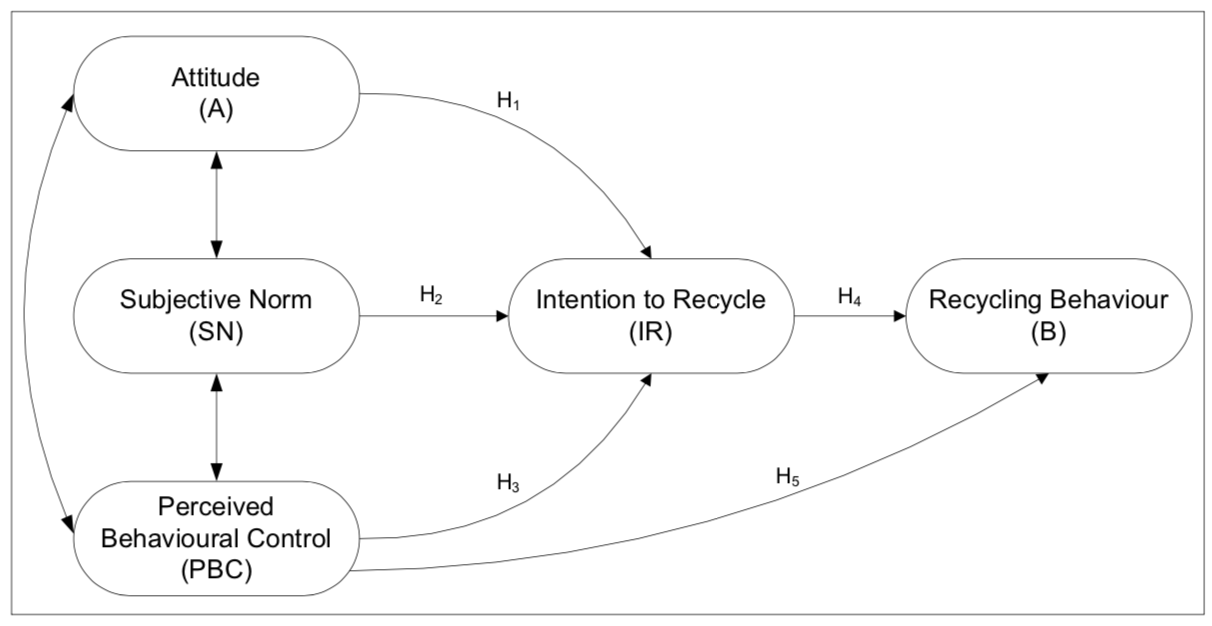
\includegraphics[width=\textwidth]{img/1/tpb-recycling.png}
\caption{The Theory of Planned Behaviour applied to recycling attitudes, norms, percieved behavioural control, intention to recycle, and actual recycling behaviour \cite{strydom_applying_2018}}
\end{figure}

Discrepancies between self-reported and actual recycling behavior are quantified at length by Huffman et. al. An issue across the field is use of the former as a proxy for the latter \cite{varotto_psychological_2017, huffman_when_2014}, due to the weak correlation between the two. However, as shown in the study, while this correlation \emph{does} exist in some cases, it is subject to a wide range of social factors and statistical limitations, including response bias and acquiescent responding, underlining the importance of conducting physical waste audits when making claims about changes in behaviour.

Hornik et. Al expand the attitude/condition model of behaviours to include both internal and external `facilitators', as well as internal and external motivators. The internal incentive is attitude, and the condition is the external facilitator: internal facilitators include knowledge and education, while external incentives are broader social-psychological effects. They found that internal facilitators such as knowledge and confidence in recycling were the best predictors of recycling behaviour, followed by external incentives. \cite{Hornik_determinants_1995}. 

\begin{marginfigure}
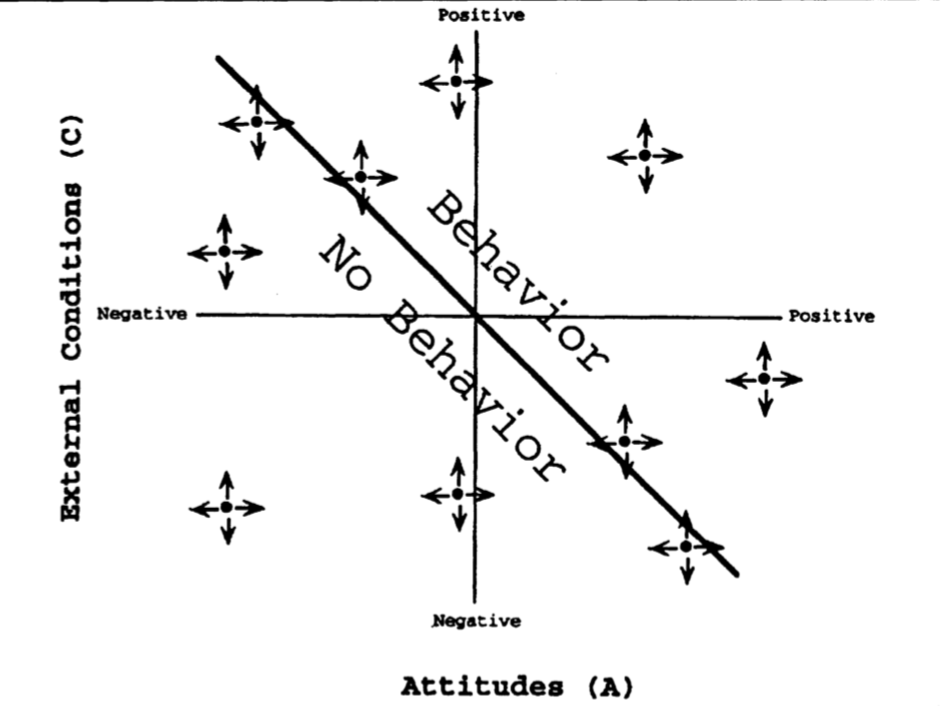
\includegraphics[width=\textwidth]{img/1/attitude-condition.png}
\caption{Stern and Oskamp's `attitude-behavior-condition' model for environmental action and participation \cite{stern_managing_1987}}
\end{marginfigure}

Kline \cite{kline_rationalizing_1988} summarises the issue: ``We would not expect individuals to engage in conservation behaviour when... personal action is not felt to contribute to the amelioration of a social problem, when the expected behaviour is regarded as cumbersome, inconvenient and ineffective, or when others who are similarly expected to conserve are perceived as not doing so''.
%more from kline?

%add to this
% %IMAGE TO ADD: hornik model
% The social environment has also been shown to play a role, with a distinction
% Importance of codesign, targeted and location (reprise in `participatory waste management' section above)

\subsection*{Building/Campus Waste Interventions}
Policy applications of this behavioural research may be found in the recently-released Zero Waste Design Guidelines, drawn up through a collaboration between AIA New York Committee on the Environment, architects Kiss + Cathcart, and environmental groups ClosedLoops and the Foodprint Group. Though many of the architectural design guidelines are specific to the structural constraints of New York, the Social and Policy recommendations draw from a range of case studies on the national and international levels \cite{aia_new_york_zero_2017}. The report outlines design solutions that incorporate both building-level and municipal interventions, though the focus is primarily on the design and adaption of individual buildings.

%IMAGE TO ADD: zwdg
\begin{marginfigure}
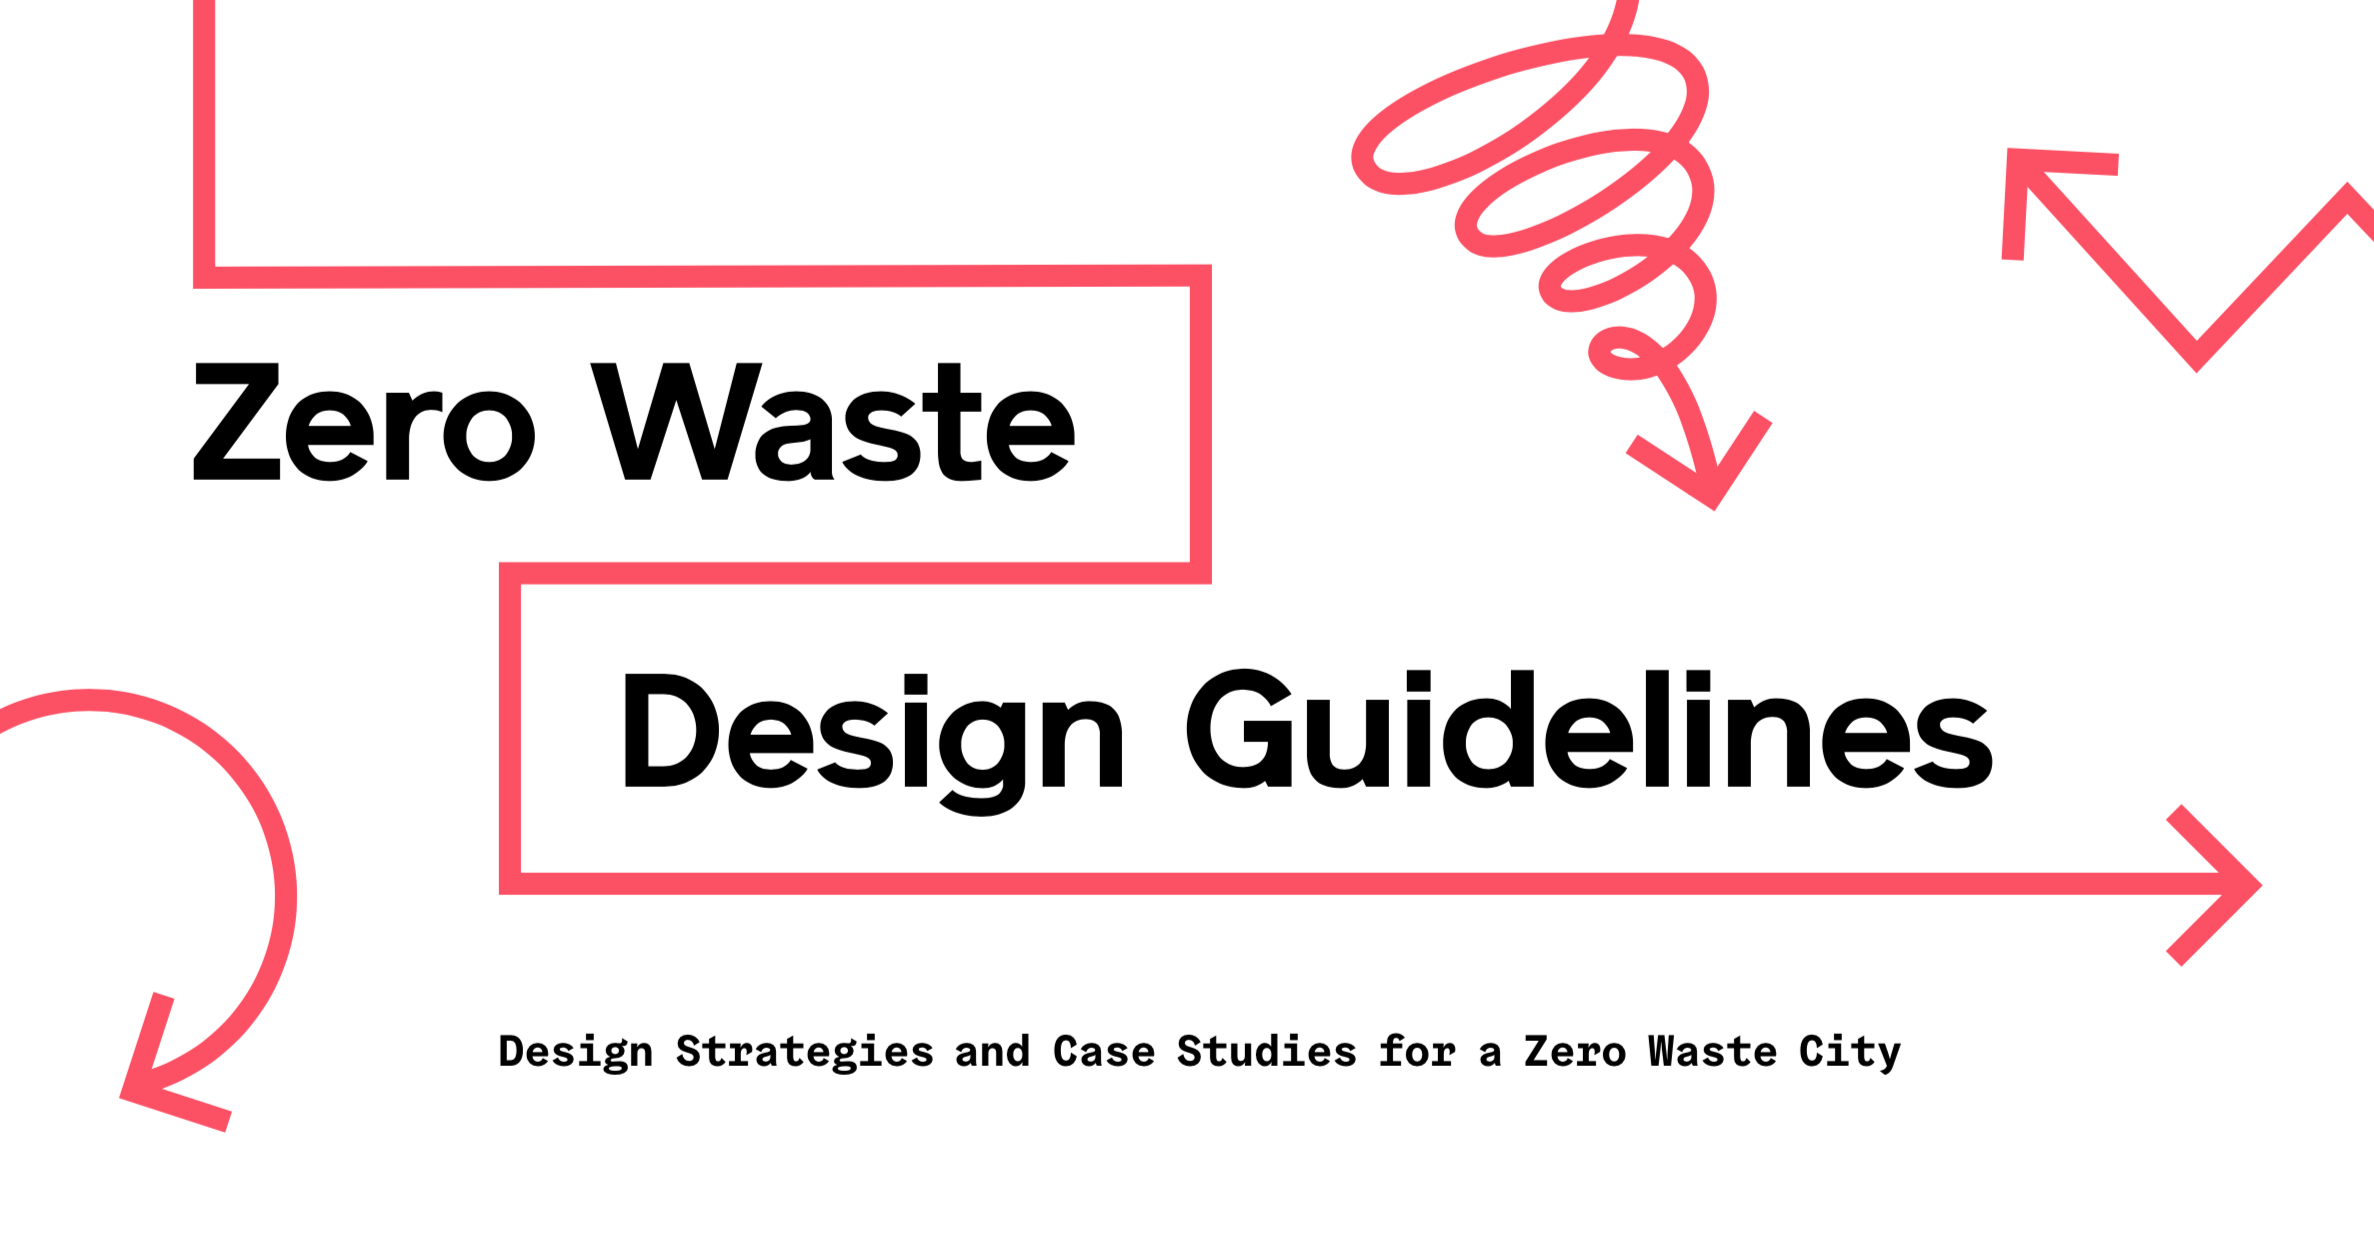
\includegraphics[width=\textwidth]{img/1/zero-waste-guidelines.png}
\caption{The Zero Waste Design Guidelines, 2018 \cite{aia_new_york_zero_2017}}
\end{marginfigure}

Interventions in the document are classified according to a set of best-practices strategies, which include a range of infrastructural, educational and participatory guidelines. One such successful intervention is the Zero Waste Program at Etsy's Brooklyn offices. Implemented in 2017 to coincide with the construction of a new building on the site, the program uses feedback on waste generation, centralised waste disposal locations, and continual waste information and education programs in addition to infrastructural changes. Among the interventions is a now open-sourced piece of software called Divertsy, which tracks the waste diverted from landfill at the offices, using a combination of user input, random audits, and automated data capture on bins.

?? explores the problem of behaviour change on the level of the university campus. In a ?? study at the ???, they ??? 

%IMAGE TO ADD: etsy intervention
\begin{marginfigure}
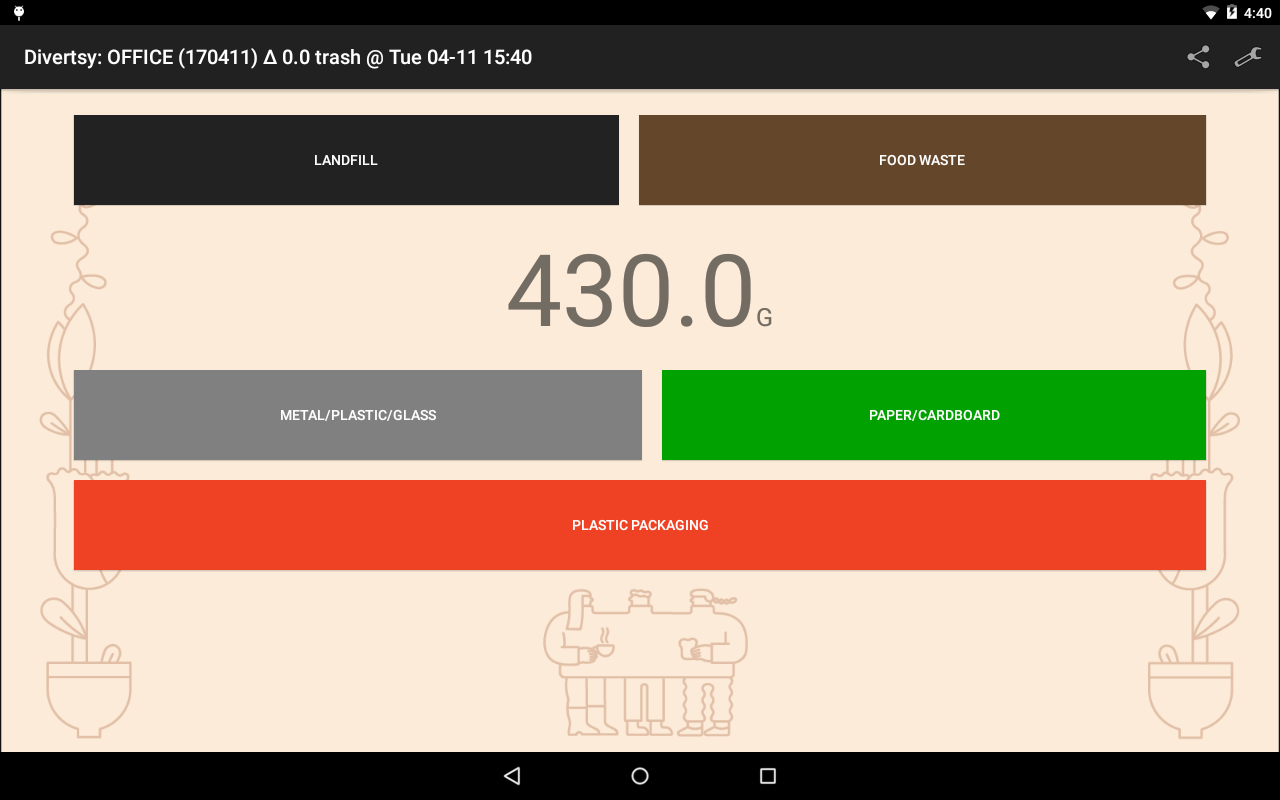
\includegraphics[width=\textwidth]{img/1/divertsy.png}
\caption{Screengrab from the Divertsy interface \cite{benninger_divertsy_2019}}
\end{marginfigure}


Throughout the report, successful case studies were highly tailored to a local context, reliant on an understanding of the specific concerns and challenges of the local populace. In Etsy's case, an audit of landfill waste from the building showed a high proportion of non-recyclable/compostable containers from local coffee shops. In response to this, the building provided staff with free re-usable cups, and provides regular information as to which vendors give a discount to customers bringing their own crockery.


\subsection*{Zero-Waste Initiatives}

An increasingly prevalent phrase in building and campus-level waste management is `zero waste', a term which has proved popular across civic and corporate spheres. The Zero Waste International Alliance describes Zero Waste as:

\begin{quote}
The conservation of all resources by means of responsible production, consumption, reuse, and recovery of all products, packaging, and materials, without burning them, and without discharges to land, water, or air that threaten the environment or human health. 
\cite{zero_waste_international_alliance_zero_2017}
\end{quote}

This develops on the rhetoric of the `recycling hierarchy' and takes a whole-system approach, in theory linking together the different contributing parts of waste streams within an institution. However, `zero waste' as a slogan can sometimes be misleading. A critique of many corporate `zero waste' initiatives is that, while investing considerable resources into campus waste management for their own offices, little attempt is made to make the actual products or industrial practices of the company more sustainable.

% \subsection*{Campus Waste Interventions}
% Campus best practices and case studies


\subsection*{Municipal Waste Interventions}

There are multiple other examples of incentive schemes that target the `external facilitators' discussed by Hornik et. al. Successful examples include 

Here, by re-framing recyclable materials as a commodity, they are given an economic value in the eyes of the consumer. Scandinavia, USA

Curbside recycling

Advertising

\section*{Taking Part in Cities}
What does it mean to take part in a civic system? If an issue in our attitudes towards and behaviours around waste is one of attention, then modes of engagement that focus attention around particular issues, dynamics and problems are of particular interest. In this section, I explore theories of participation, with a focus on the use of games and play as a means of making legible otherwise dull, inaccessible or obscure processes. While here I explore ideas within the field of urbanism, these concepts may also be applied to other forms of civic and political participation.

\subsection*{Participatory Urbanism and Co-design}

\begin{flushright}
\emph{``Technology is the answer, but what was the question?''} \cite{price_technology_1979}\\
Cedric Price
\end{flushright}

Participatory urbanism draws from ideologies around advocacy, equity and transactive planning as an increasingly common paradigm through which large-scale civic projects are framed \cite{krivy_participatory_2013}. At its core, participatory urbanism is intended to give a voice to those affected by planning practices, and to promote political equality through giving under-represented groups agency over their environs. `Participatory' is, however, a notoriously over-used phrase, describing a continuum of practices ranging from radical co-operatives through to the proponents of the `sharing economy', where invocations of participation can veer toward the exploitative. Alphabet Inc's Sidewalk Labs, for example, has been criticised for using a `participatory' input process that restricts range of possible responses as a substitute for real civic democracy. When it is not possible to question the basic assumptions of the design process, participation becomes less about `democratic planning' and more about symbolic or tokenistic involvement \cite{arnstein_ladder_1969}. Increasingly, practicioners in the field use the phrase `co-design' in place of `participatory design', due to the negative connotations that the latter has accrued.

\subsection*{Participation in Waste Management}
\begin{flushright}
\emph{``[W]here we cannot redirect the wasting process, we must change our minds''}\cite{lynch_wasting_1990} \\
Kevin Lynch
\end{flushright}

A key idea in participatory urbanism is that ownership of and participation in the management of a system can increase the effectiveness of various interventions to that system. Forms of participatory waste management range from digital reporting systems \cite{offenhuber_waste_2017}, to community work with recycling collectors \cite{tremblay_united_2010, mundano_pimp_nodate}, to actively engaging volunteers in recording and managing waste streams, and educating their peers \cite{offenhuber_waste_2017}. 

\begin{marginfigure}
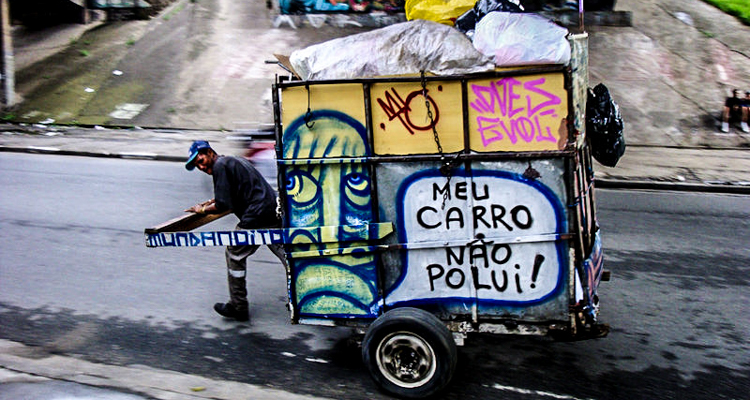
\includegraphics[width=\textwidth]{img/1/catadores.jpg}
\caption{An image from Thiago Mundano's project \emph{Pimp My Carro\c{c}a}, where recycling workers (\emph{catadores}) in S\~{a}o Paulo are paired with local artists who paint their carts, while also offered free healthcare and safety equipment. This participatory project was started to underline the work that the \emph{catadores} do to keep the city clean. \cite{mundano_pimp_nodate}}
\end{marginfigure}

In \emph{Waste is Information}, Offenhuber examines the role of interfaces between citizens and governments in `participatory' waste collection systems, making the argument that the politics of representation of a system require a set of common protocols, understood by all participants. Using the example of a participatory waste project in Boston, where infratructure failures were crowdsourced from residents through a mobile app, he critiques the notion of decentralisation for decentralisation's sake, arguing that the fragmentation of urban services can create the kind of inequality it might purport to dynamically address \cite{offenhuber_waste_2017}. Jennifer Gabrys, too, explores how well-meaning citizen science projects can nonetheless end up using people as a cheap means of producing data for somebody else, rather than projects that give back as much as they demand from participants. \cite{Gabrys_programming_2014}

%IMAGE TO ADD: trash track
\begin{marginfigure}
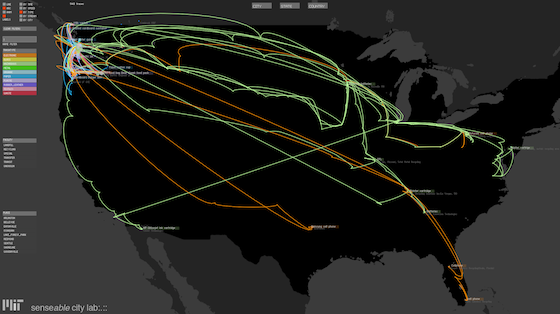
\includegraphics[width=\textwidth]{img/1/trashtrack1.png}\\
\vspace{0.5cm}
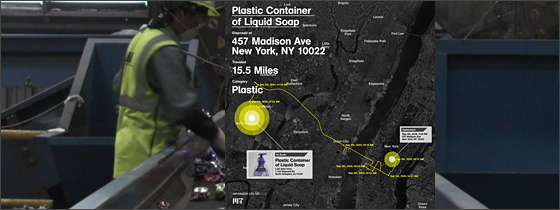
\includegraphics[width=\textwidth]{img/1/trashtrack2.jpg}
\caption{Visualisations from the Trash Track project \cite{ratti_trash_2009}}
\end{marginfigure}

In 2009 Offenhuber worked on MIT Senseable City Lab's Trash Track project \cite{ratti_trash_2009}, which used a set of GPS sensors, installed by volunteers to track the movement of different kinds of waste emanating from the city of Seattle. This project provided a detailed insight into the variety of destinations reached, routes and time taken to get there, as well as an analysis of how effectively the different kinds of waste were being dealt with. The insights were then communicated back to volunteers and the wider community as a series of visualisations, tracing the path of individual objects and types of waste, and comparing their eventual destinations to those reported by the local authority.

\begin{marginfigure}
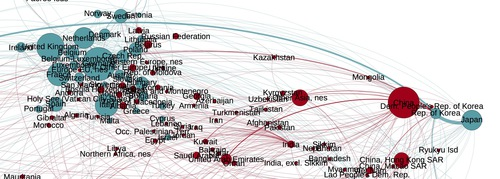
\includegraphics[width=\textwidth]{img/1/lepwasky-ewaste-flows-2012.jpg}
\caption{Josh Lepawsky's visualisation of e-waste flows}
\end{marginfigure}

Projects such as this, and Josh Lepawsky's E-Waste visualisations \cite{lepawsky_changing_2015} are both key in making visible hidden infrastructures and externalities within waste systems. In particular, Liboiron argues, it is in showing these complex geographies that popular misconceptions of waste might be changed \cite{liboiron_mapping_2014}. However, these visualisations stop a little short of asking the viewer to take responsibility for their role within a system. As `views from nowhere', they do not include the viewer themselves, allowing one to dissociate the movement of this waste from one's own role within the system of its production.

This is a point explored by Schamin\'ee, who discusses the importance of representing the audience in interventions targeted toward them. In a discussion of a campaign in the Netherlands to raise awareness about Climate Change, Schamin\'ee writes that ``There are no polar bears and deserts in the Netherlands, and citizens can't control what comes out of a factory chimney... we had to find out what climate change means to the everyday lives of residents in the here and now''. \cite{schaminee_designing_2018}

\subsection*{Space, Place and Waste}
\begin{flushright}
\emph{The space in which we live... is also, in itself, a heterogeneous space. In other words, we do not live in a kind of void, inside of which we could place individuals and things... we live inside a set of relations that delineates sites which are irreducible to one another and absolutely not superimposable on one another.''}\cite{foucault_other_1967}\\
-- Michel Foucault
\end{flushright}

What forms of representation can address civic issues in context? One idea emphasised by participatory approaches is the importance of local knowledge and culture in interventions in civic systems. Charlie DeTar distinguishes between space as a geometry of location, and place as the interpretation of that location. He argues for context-aware technologies that are sensitive to the people and culture within a location, rather than purely the space itself. ``Rather than being composed of purely structural elements, places are relational'' \cite{detar_mapping_2011}.

In \emph{Local Codes: Forms of Spatial Knowledge} Shannon Mattern argues that public institutions such as libraries and community centres -- with access to specific forms of local knowledge -- are best placed to deal with engaging diverse publics, new urban technologies, and infrastructural change \cite{mattern_local_2019}. Urban designer Usman Haque emphasises the importance of local decision-making when it comes to creating cultural interventions, asserting that collective and place-based forms of engagement are key in fostering lasting forms of civic participation \cite{haque_citizen_2017, haque_notes_2008}. 

Ideas of place feature heavily in Kevin Lynch's work, whose cognitive mapping techniques take at their core the highly subjective and shifting relationship between people and their percieved environments. In \emph{The Image of the City}, Lynch argues that infrastructural legibility is constructed in ``a two-way process, between the observer and his environment'' \cite{lynch_image_1960}.

In \emph{Postmodernism}, Frederic Jameson reflects on what Lynch's cognitive mapping might look like for an era in which technology `no longer possesses this same capacity for representation' as Lynch's cities did in the 1960's. Describing Lynch's approach as ``pedagogical political culture which seeks to endow the individual subject with some new heightened sense of its place in the global system'', he calls for new forms of cognitive mapping, on a ``social as well as a spatial scale''. \cite{jameson_postmodernism_1991}.


\section*{Playful citizenship}

\begin{flushright}
\emph{Since everyone knows what a map is, it would have been necessary to add that cognitive mapping cannot (at least in our time) involve anything so easy as a map}\cite{jameson_postmodernism_1991} \\
-- Frederic Jameson
\end{flushright}

%procedural rhetoric: bogost: arguments made by computer programs
%make a much stronger arfument here for games and systems. cite macklin, tseng and others
In \emph{WORLD CLIMATE: A Role-Play Simulation of Climate Negotiations}, Sterman et. al make the case for representing climate change through simulation, as it is impossible to learn from either controlled experiments, or experience \cite{sterman_world_2015}. Colleen Macklin of the New School's PETLab also makes the case for simulation and role-play in \emph{Games for a New Climate}, in which she worked with the Red Cross/Red Crescent to make playful simulations of decision-making in the context of climate-related disasters. Macklin terms games as the `pop cultural medium of systems', a mode of participatory simulation that comprises ``one of the more important strategies for connecting knowledge to action'' \cite{macklin_games_2013}.

\begin{marginfigure}
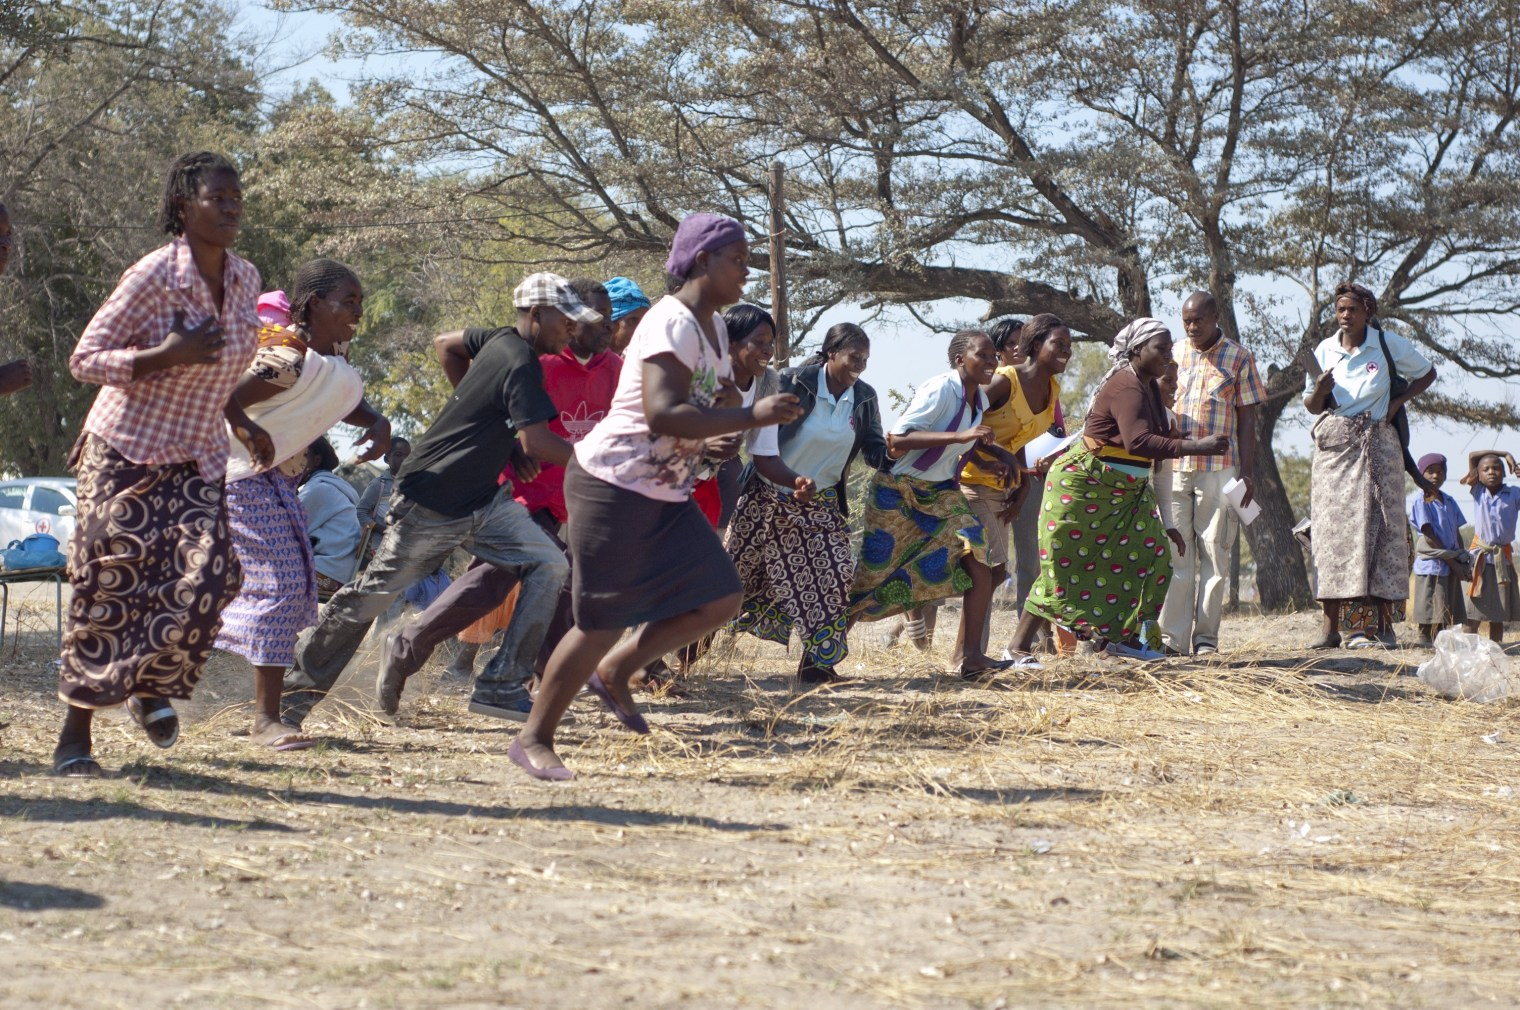
\includegraphics[width=\textwidth]{img/1/macklin-climate.jpg}
\caption{A photograph of gameplay from Colleen Macklin's \emph{Games for a New Climate} in Katima Mulilo, Namibia \cite{macklin_games_2013}}
\end{marginfigure}

'Serious' or `civic' games (here I choose the latter term) and simulations have become an increasingly popular mode of engagement for participatory projects in recent decades \cite{krivy_participatory_2013}. While there are numerous use cases for these games, here I will focus on games intended specifically for the context of urban planning and infrastructure legibility. At their core, the `civic games' of interest here are modes of play that make legible complex infrastructural systems (be they physical, political, or social) through participatory, critical and exploratory methods.
%In his talk ???, Francis Tseng ???Nicky Case, Colleen Macklin, Sterman
%argumwnt goes here 

% \begin{marginfigure}
% 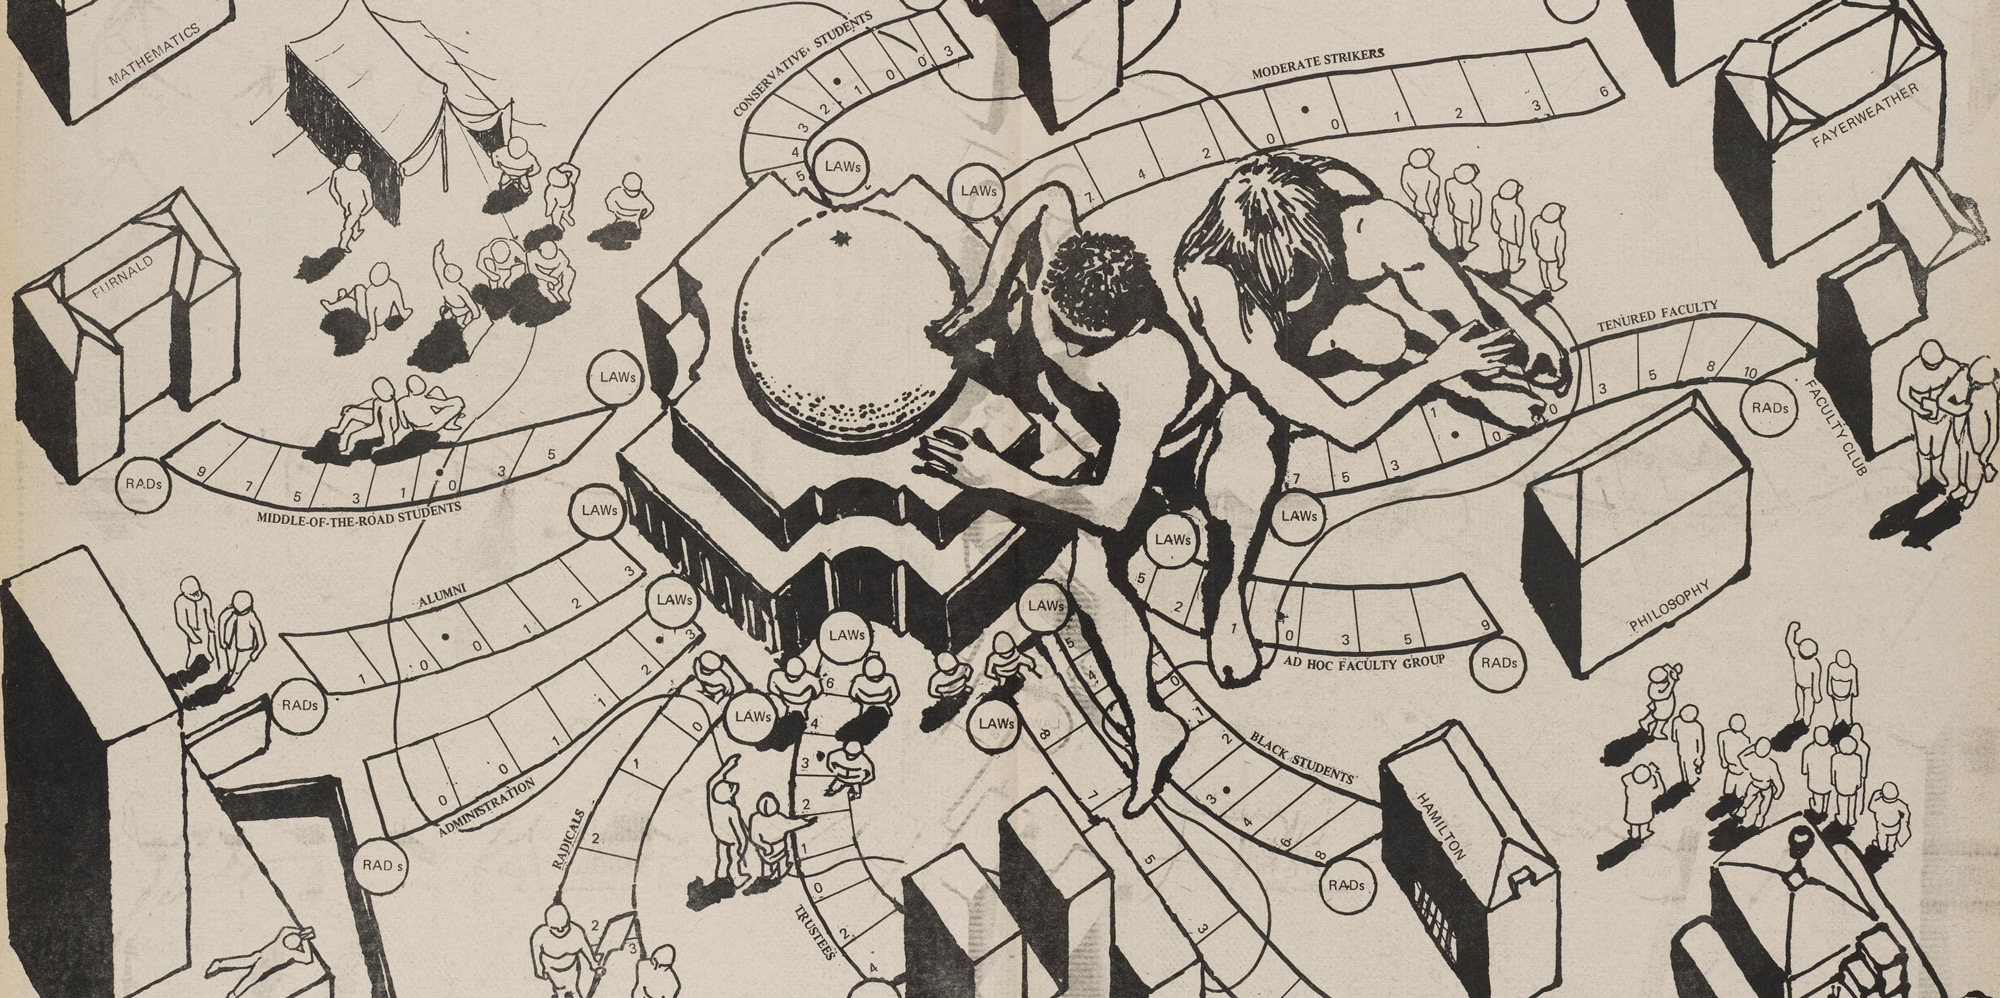
\includegraphics[width=\textwidth]{img/1/up-against-the-wall-motherfucker.jpg}
% \caption{The board from Jim Dunnigan and Jerry Avorn's \emph{Up Against The Wall, Motherfuckers \cite{dunnigan_few_1969}}
% \end{marginfigure}
%add a sentence before `assuming'
%making democracy fun
The `simulation video game' as a consumer product originates from the late 1980s, when games such as SimCity proved surprisingly popular amongst players, though simulation games themselves have a much longer history. Arguably, strategic `war games' are some of the oldest forms of simulation game, with games such as Prussian King Frederick the Great's \emph{Kriegsspiel} used as strategic tools from the early \nth{19} Century. \cite{landa_war_1991}

In the 1960's, the simulation game gained popularity as a management and learning tool, appearing in the US Military's `Operations Research' archives\cite{landa_war_1991}, in the `World Game' proposed by Buckminster-Fuller\cite{buckminster_fuller_institute_about_nodate}, as a utopian activist tool \cite{johnson_inside_2013}, and as satirical commentary on current affairs\cite{dunnigan_few_1969}.
%\sidenote{Jim Dunnigan's \emph{Up Against the wall, Motherfuckers} is one such example: a simulation game that modelled possible outcomes of the previous years' campus occupation at Columbia University, led by the eponymous anarchist group. The game was included as a supplement to the April 1969 edition of the Columbia Daily Spectator \cite{dunnigan_few_1969}} 
Contemporaneous with the emergence of participatory planning, 1960s activist organisations such as the New Games Movement saw games as a tool for direct action, as well as systems simulation \cite{johnson_inside_2013}. 

\subsection*{Participatory Simulation}

\begin{flushright}
\emph{``I could never have told them that and had any impact. They had to discover it for themselves.''}\cite{sterman_john_2013}\\
John Sterman
\end{flushright}

In the case of simulation, games can form a popular medium for modelling: a way for people not just to simulate a system to learn about its workings, but to actively participate in playing out the consequences of particular courses of action. SimCity is often credited for inspiring a generation of urban planners captivated by their role in a simulated local government \cite{roy_video_2019}. However, as a tool of representation, these games are not neutral: common critiques of SimCity are that it assumes an urban system planned and controlled from above, and that the closed nature of the underlying algorithm, a `black box' does not allow the player to question the underling assumptions of the game's maker \cite{starr_seductions_1994}.

\begin{marginfigure}
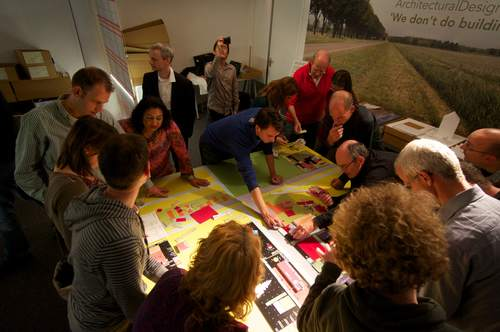
\includegraphics[width=\textwidth]{img/1/play-oosterwald.jpg}
\caption{Participants in the City Game `Play Oosterwald', a participatory planning exercise to design a new, green town in the Municipality of Almere, Netherlands \cite{play_the_city_play_2013}}
\end{marginfigure}

In her book \emph{Negotiation and Design for the Self-Organising City}, architect Ekim Tan asks us to re-consider urban games (such as SimCity) in a more open-ended context, advocating for `city gaming' as an accessible tool for engaging communities in urban planning exercises \cite{tan_negotiation_2014}. Tan's city games occupy a spectrum between educational and planning tools, including awareness-raising exercises about mass migration, educational games about successful affordable housing policies, and consultation on making new developments more bicycle- and pedestrian-friendly. \emph{Play the City} is intended to `accelerate consensus' between stakeholders with conflicting interests, bringing together citizens, planners and policymakers in collective decision-making exercises, constrained by a rule-set that is tailored to the problem they are trying to solve \cite{tan_city_2017}. However, in generating the rules of the game, the asking of more basic questions e.g. `Should this development exist in the first place' is essential for true (rather than tokenistic) democracy \cite{shaw_informational_2017}.

\begin{marginfigure}
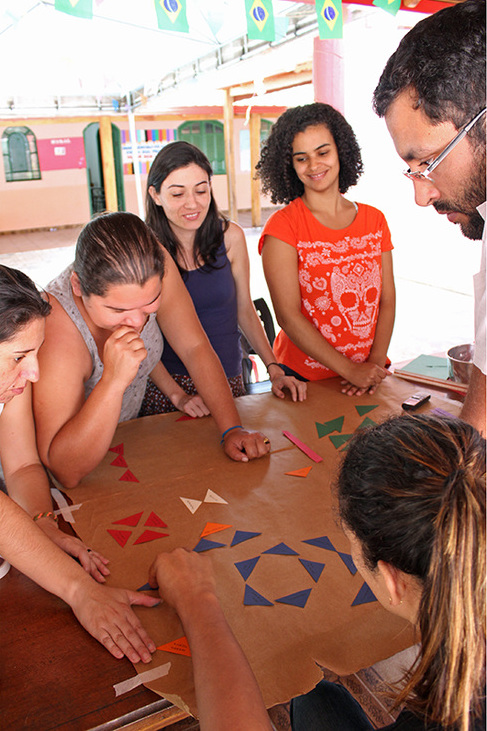
\includegraphics[width=\textwidth]{img/1/usina-triangles.jpg}
\caption{A participatory planning exercise organised by USINA CTAH as part of an agro-ecological planning project southernmost region of Bahia, Brazil. This part of the exercise -- ``activity of the triangles'' -- uses more abstract forms of planning to remove existing hierarchies  \cite{noauthor_usina_ctah_nodate}}
\end{marginfigure}

More explicitly political in nature are organisations such as the Brazilian architectural practice USINA Centro de Trabalhos para o Ambiente Habitado (``Work Center of the Inhabited Environment"), who use similar techniques of rules and games to work directly to advocate for residents' and workers' rights in the construction of new developments. Using similarly rule-based and physical co-design techniques, USINA work directly with communities, developing construction processes optimise for construction workers' safety, and working with homeless and displaced people \cite{noauthor_usina_ctah_nodate}.

%some more joining here, maybe rosario
Building on a history of participation techniques across both Latin America and the USA, Josh Lerner's \emph{Making Democracy Fun} explores the use of game design principles in democratic participation, making a distinction between games as \emph{metaphor}: games used to explain and represent political processes, and games as \emph{method}: making the political process a game in and of itself \cite{lerner_making_2014}. %rosario here!

Participatory simulations such as John Sterman's \emph{World Climate} scenarios sit somewhere between metaphor and method, using complex climate models to guide participants (typically politicians, policymakers and academics) through a range of scenarios. 
\begin{marginfigure}
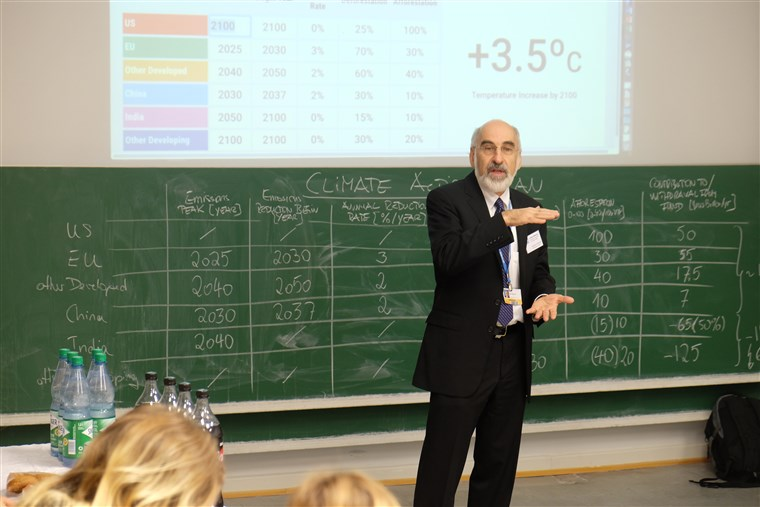
\includegraphics[width=\textwidth]{img/1/sterman-climate.jpg}
\caption{John Sterman running a session of \emph{World Climate} \cite{sterman_john_2013}}
\end{marginfigure}
Based directly on climate science, \emph{World Climate} seeks to get participants to `draw their own conclusions', about emissions policy, rather than attempt to argue the point with words \cite{sterman_john_2013}. While these games might not be directly used as part of the decision-making process, their deployment is more than simple awareness-raising, as often the audience they engage has a direct effect on the system described.


\subsection*{Critical Games}

The works of Francis Tseng and Frank Lantz both provoke critical narratives within simulation games. For example, Lantz's wildly popular \emph{Universal Paperclips} provides an insight into the perils of ill-constrained artificial intelligence \cite{lantz_universal_2017}, while Tseng's startup simulator \emph{The Founder} satirises unethical innovation processes \cite{tseng_founder_2017}. In both these cases, a compelling narrative (supported, in Lantz's case, by a fairly bare interface) is used to involve the player in participating in a simulation.

\begin{marginfigure}
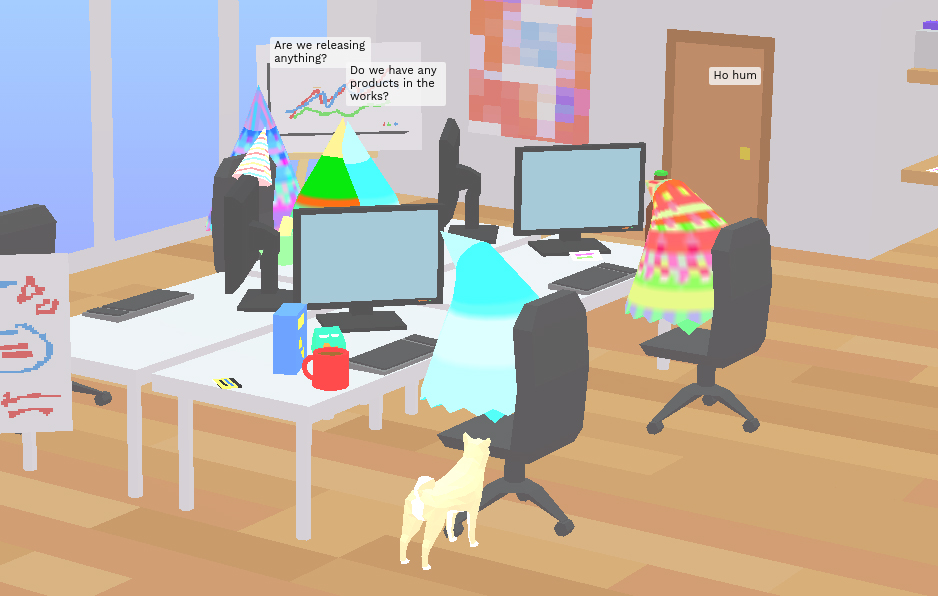
\includegraphics[width=\textwidth]{img/1/the-founder.jpg}
\caption{A still from Francis Tseng's `Dystopian business simulator' \emph{The Founder} \cite{tseng_founder_2017-1}}
\end{marginfigure}

The performance of these transgressive behaviours within the game setting encourage the player to think more critically about what aspects of the system led them to behave in the way that they did: a technique that combats what Scot Osterweil terms the `virtuous player syndrome' (where players unquestioningly do what they assume is `right' in order to win the game) \cite{osterweil_civic_2011}.

\begin{marginfigure}
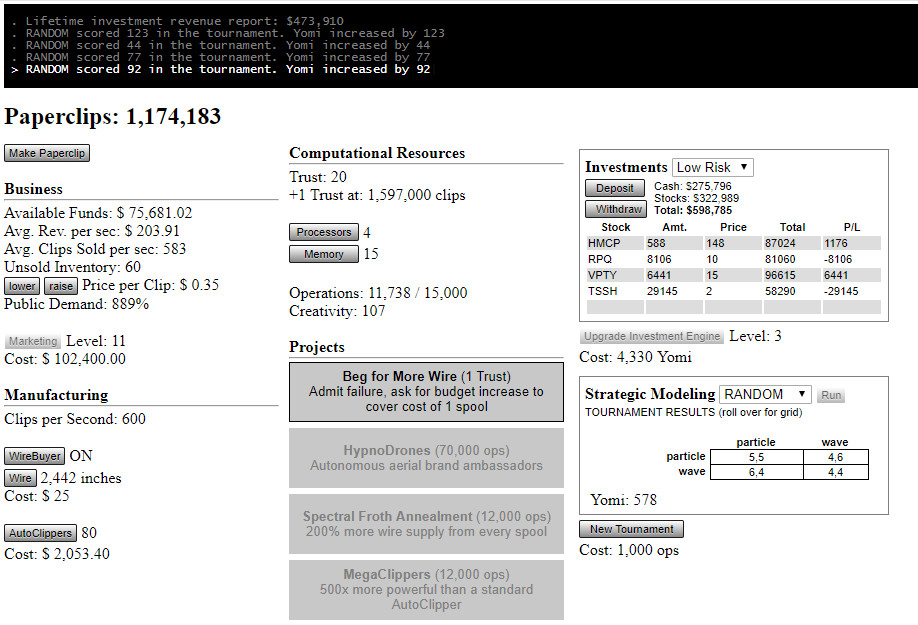
\includegraphics[width=\textwidth]{img/1/universal-paperclips-progress.jpg}
\caption{A still from Frank Lantz's \emph{Universal Paperclips} \cite{lantz_universal_2017}}
\end{marginfigure}

James Gee's \emph{What Video Games have to teach us about Learning and Literacy} provides a foundational framework for understanding how games can be used to encourage critical thinking about a particular issue. Gee outlines a set of 30 principles core to games from which a player can learn, including the `cultural models' principle (in which players are encouraged to reflect on the model with which they view the world), the `self-knowledge' principle (whereby a game is constructed such that players may learn about themselves as well as the domain of the game) and the `situated meaning' principle, in which actions in the game have bearing on real-world actions \cite{gee_what_2004}. Gee also advocates for co-design -- the participation of stakeholders -- in all stages of the game's development.

\subsection*{Explorable Explanations}
Another core theme of Gee's writing is the ability of players to explore the principles underlying the function of games, and to modify and extend their experience of them. Nicky Case's simulation games -- which use Bret Victor's term `explorable explanations' -- act as sandboxes for the player, allowing them to question the assumptions underling their models. Case encourages players to perturb the dynamics of a complex system, both to learn, and then to test the assumptions made by the game's author \cite{case_how_2016}. Case cites Donella Meadows as a key inspiration in their work, which sits between systems theory, simulation and play.

As Ava Kofman argues, on writing about agency in urban simulation games ``We should ask not what our ideal city on SimCity, LivingPlanIT, or some other Urban OS would look like, but what our ideal urban simulator would be. Given this or that operating system, who does the city work for and who works for the city? No longer is the goal to design an urban imaginary: you must now code the game.''.

\begin{marginfigure}
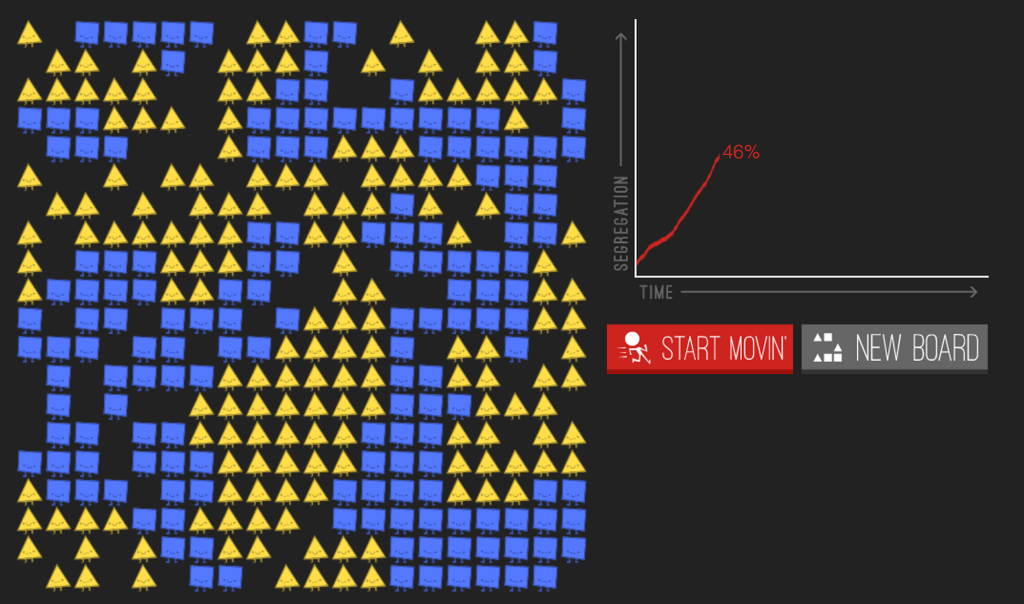
\includegraphics[width=\textwidth]{img/1/parable.png}

\vspace{0.2cm}

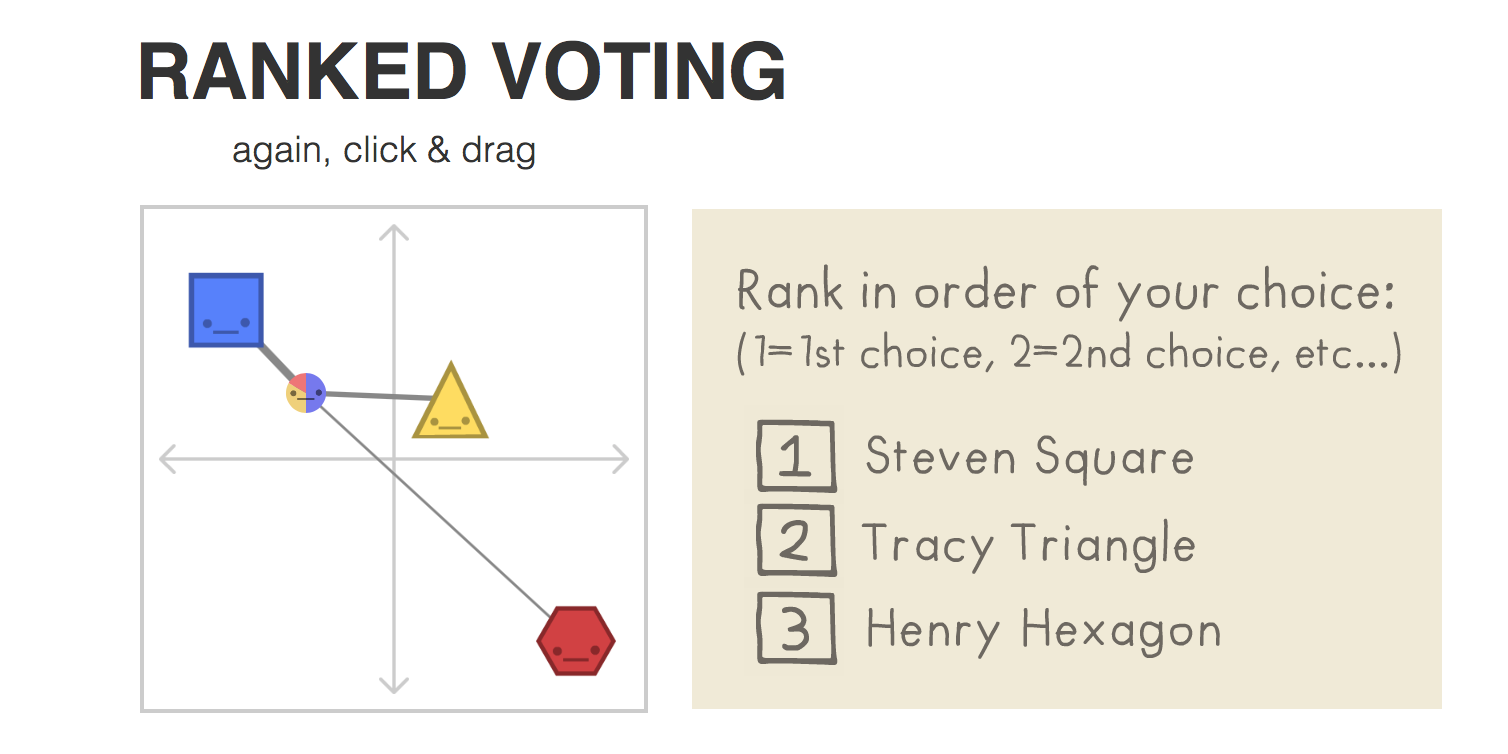
\includegraphics[width=\textwidth]{img/1/voting.png}
\caption{Vi Hart and Nicky Case's \emph{Parable of the Polygons} (top) creates an explorable version of Schelling's segregation models, allowing the player to modify the parameters of the simulation \cite{case_parable_2015}. Case's \emph{To Build a Better Ballot} (bottom) uses these ideas to give the user a critical, interactive exploration of the effects of complex voting policy \cite{case_build_2016}.}
\end{marginfigure}

\subsection*{Playing with Trash}

\begin{flushright}
\emph{``so i've been playing this game the last few days and it's such a love hate thing... my city was just starting to blossom... and then guess what --- people stopped working at my sewage plant and my garbage fill because they weren't ``low income'' workers anymore... so slowly garbage and shit starting filling the streets and everyone abandoned the city like i'm about to abandon the game again. thanks.''}\cite{friedricekid_is_2017}\\
-- Reddit user friedricekid reviewing SimCity 2013
\end{flushright}

%make this a bit more interesting: what are these games trying to achieve?
%how do they do it?
While there are some existing games about waste, it is hard to find any framed around the players' participation in urban infrastructure that give a critical perspective on the waste system. Many waste games take the form of `recycling sorting' games: players are tasked with sorting waste items into requisite bins, under some time constraint, or, in more elaborate scenarios, in the context of a relay. Players are scored as to the amount of waste they sorted successfully, testing their knowledge of different waste categories. 

%IMAGE TO ADD: garbage dreams
\begin{marginfigure}
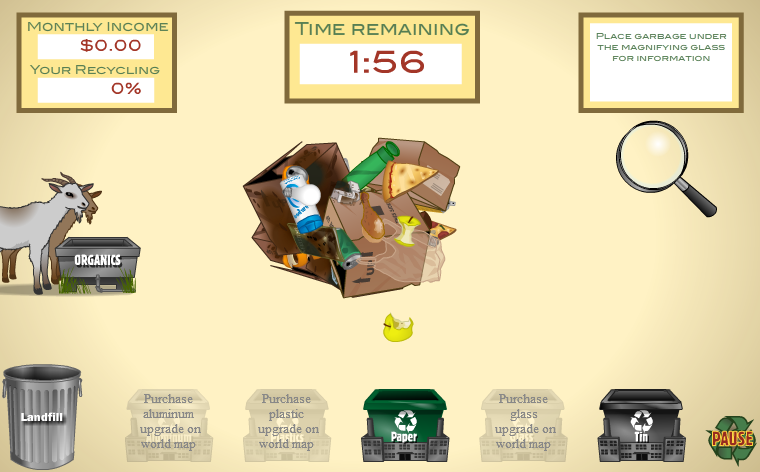
\includegraphics[width=\textwidth]{img/1/garbage-dreams-1.png}
\caption{Sorting trash in PBS's \emph{Garbage Dreams} \cite{iskander_garbage_2011}}
\end{marginfigure}

PBS's Garbage Dreams gives a narrative to this sorting: playing the role of a Zaballeen (a waste-sorter in Cairo), the player is tasked with building out waste-sorting empire, purchasing better equipment and educating locals to increase the efficiency of the sorting program \cite{iskander_garbage_2011}. Garbage Dreams is effective in using a simple game mechanic, and slowly increasing the complexity of the game, illiustrating the challenges in sorting complex waste streams. 

Hirose et. Al's Industrial Waste Game \cite{hirose_industrial_2004} -- a card game that highlights the challenges and social dynamics of waste monitoring -- is the subject of a study on environmental education. Specifically, by using a systems-simulation approach to the problem of waste monitoring, the game was shown to help change attitudes towards people dumping waste illegally, seeing this as the product of a social (rather than a psychological) context. 

In the context of urban simulation games, SimCity 2013 included solid waste management as a part of a complex urban simulation (incidentally, this is also the first edition of the game to include `people' in the model). This game mechanic focussed primarily on pollution as a feedback system: allowing waste to pile up makes simulated citizens unhappy, but so does higher rates of air pollution from burning it. As in the above quote, aspects of the waste mechanic (plus numerous bugs) meant that the game proved unpopular to players, and the game garnered poor reviews.  

While SimCity is often used as an educational tool by urban planners and local governments \cite{gaber_simulating_2007, lobo_city_2004}, it has been criticised for a `largely aesthetic' \cite{gaber_simulating_2007} rendering of its citizens, where the player can only lose if they run out of money, and rarely has to deal with the consequences of civic dissatisfaction. 


%IMAGE TO ADD: sim city 2013
\begin{marginfigure}

\includegraphics[width=\textwidth]{img/1/simcity2013-recycling.jpeg}
\caption{A recycling plant from SimCity 2013 \cite{noauthor_garbage_2013}}
\end{marginfigure}


\begin{quote}
\emph{...shouldn’t a game with so much influence on future planners and citizens not just teach power accumulation, but at least attempt to instill a sense of what government can and should do -- some sense of values transcending simple supply and demand that underlie planning?} \cite{lobo_city_2004}\\
Daniel Lobo
\end{quote}

Of course, one could argue that critical learning and political agency are not necessarily what SimCity is going for. As Lobo puts it:``Forgetting the irony and playfulness of SimCity in the classroom would equal to teaching civic behavior with fighting games such as Mortal Kombat, Quake or Tekken IV'' \cite{lobo_city_2004}. Nonetheless, this remains a key distinction between the work described here, which seeks specifically to contextualise the players' role in the waste system.

Despite numerous examples, it is hard to find a civic game concerning waste that has been tied to a specific local context. Garbage Dreams, for example, is set in Egypt, but the only version of the game online is in English, underlining the idea that wastes are dealt with `somewhere else'. Likewise, the undergraduate students that comprised the primary subjects of Hirose et. al's study are likely not those directly involved with industrial waste disposal. 

Why might this matter? For one, decontextualised `awareness-raising' games might shape the discourse around an issue, but if the goal of such games is to lead to action on behalf of the audience, then players should be able to relate their actions in the real world to events in the game itself. In a critique of games that simply `raise awareness', Lerner declares that the greatest limitation of the `social issues game' is a ``tenuous connection to politics and community groups... [they] tend to have hazy goals and rarely help translate awareness into action'' \cite{lerner_making_2014}. This not to say, of course, that there is nothing to be learned by playing these games, nor that locally contextualised games cannot be generalised in many aspects. However, this thesis posits that reference to and interaction with the infrastructural context of the players is necessary for games to link a change in awareness to one of attitude and behaviour.

\subsection*{Conclusions}
Waste systems suffer from a crisis of representation, in part because they are complex, and hard to represent, and in part because when they are made visible, there is a cultural attitude toward them that lacks care and attention. A whole-systems perspective on waste could highlight the impact of behaviours such as recycling contamination, which stems from a combination of good intentions and a lack of information. Examples of representation in other such complex systems (climate change \cite{sterman_world_2015, macklin_games_2013}, democratic participation \cite{lerner_making_2014, case_build_2016}) show that simulation and games can be a powerful tools for engaging civic attention around otherwise difficult issues.

Understanding and information need to come alongside infrastructural change when making interventions in municipal waste systems \cite{kline_rationalizing_1988}. Serious games give us both a means of making legible complex systems, and in engaging stakeholders in critical awareness, participation and action. Using waste as a case study, and building on existing models for designing with public organisations \cite{schaminee_designing_2018}, this thesis provides a framework for making explicit the connection between context, awareness and action in civic games.


%General awareness-raising without reference to specific infrastructural concerns might shape the attitudes of players towards a topic, but, if we consider the findings of Stern et. al, might be unlikely to affect a behavioural change.

%why might it be important to tie a game to a specific local context? What difference does that make? ?? Keller??

\chapter{Understanding Waste at MIT}

Taking the need for infrastructure legibility of waste systems as a point of departure, this thesis proposes that civic games can be used in the context of broader infrastructural change as a critical, participatory and open-ended educational tool.

This work is being done alongside the Zero Waste pilot program in the Media Lab, itself part of a campus-wide scheme to more sustainably manage waste on campus. In the first part of this section, I will outline the structure and aims of this pilot study, and discuss its relationship to this project. In the second part of this section, I will describe and present the results of a series of interviews conducted with various stakeholders in the MIT waste system, alongside discussions from the pilot project meetings, and results from the pilot outreach and feedback sessions. From these discussions, I will draw out a set of clear themes, which are used to meet the goals defined in part 1, and outline a proposal for the thesis.

\section*{Waste at MIT}

Solid waste management at MIT is handled by Custodial Services, and the Office of Recycling and Materials Management, both of which fall under the umbrella of `Campus Services', which also includes bodies such as the Mail Rooms, and Grounds Services. A separate, contracted service is used to handle solid waste management in residential dormitories on campus. For the sake of simplicity, only the main waste management bodies are considered here. Throughout this project, the people I worked most closely with were Ruth Davis (manager of the Office for Recycling and Materials Management), Brian Goldberg (Sustainability Project Manager at MITOS), and with Tom Hardy (manager of Custodial Services).

Custodial Services is considerably larger than the Office of Recycling, employing just under 180 staff, the majority of whom (around 135), are employed on a night shift. By contrast, the Office of Recycling employs just 5 recycling movers, who are tasked with collecting recycling from all of the 20 campus loading docks, and transporting it to Casella, the MRF used by MIT. 

\begin{figure*}
 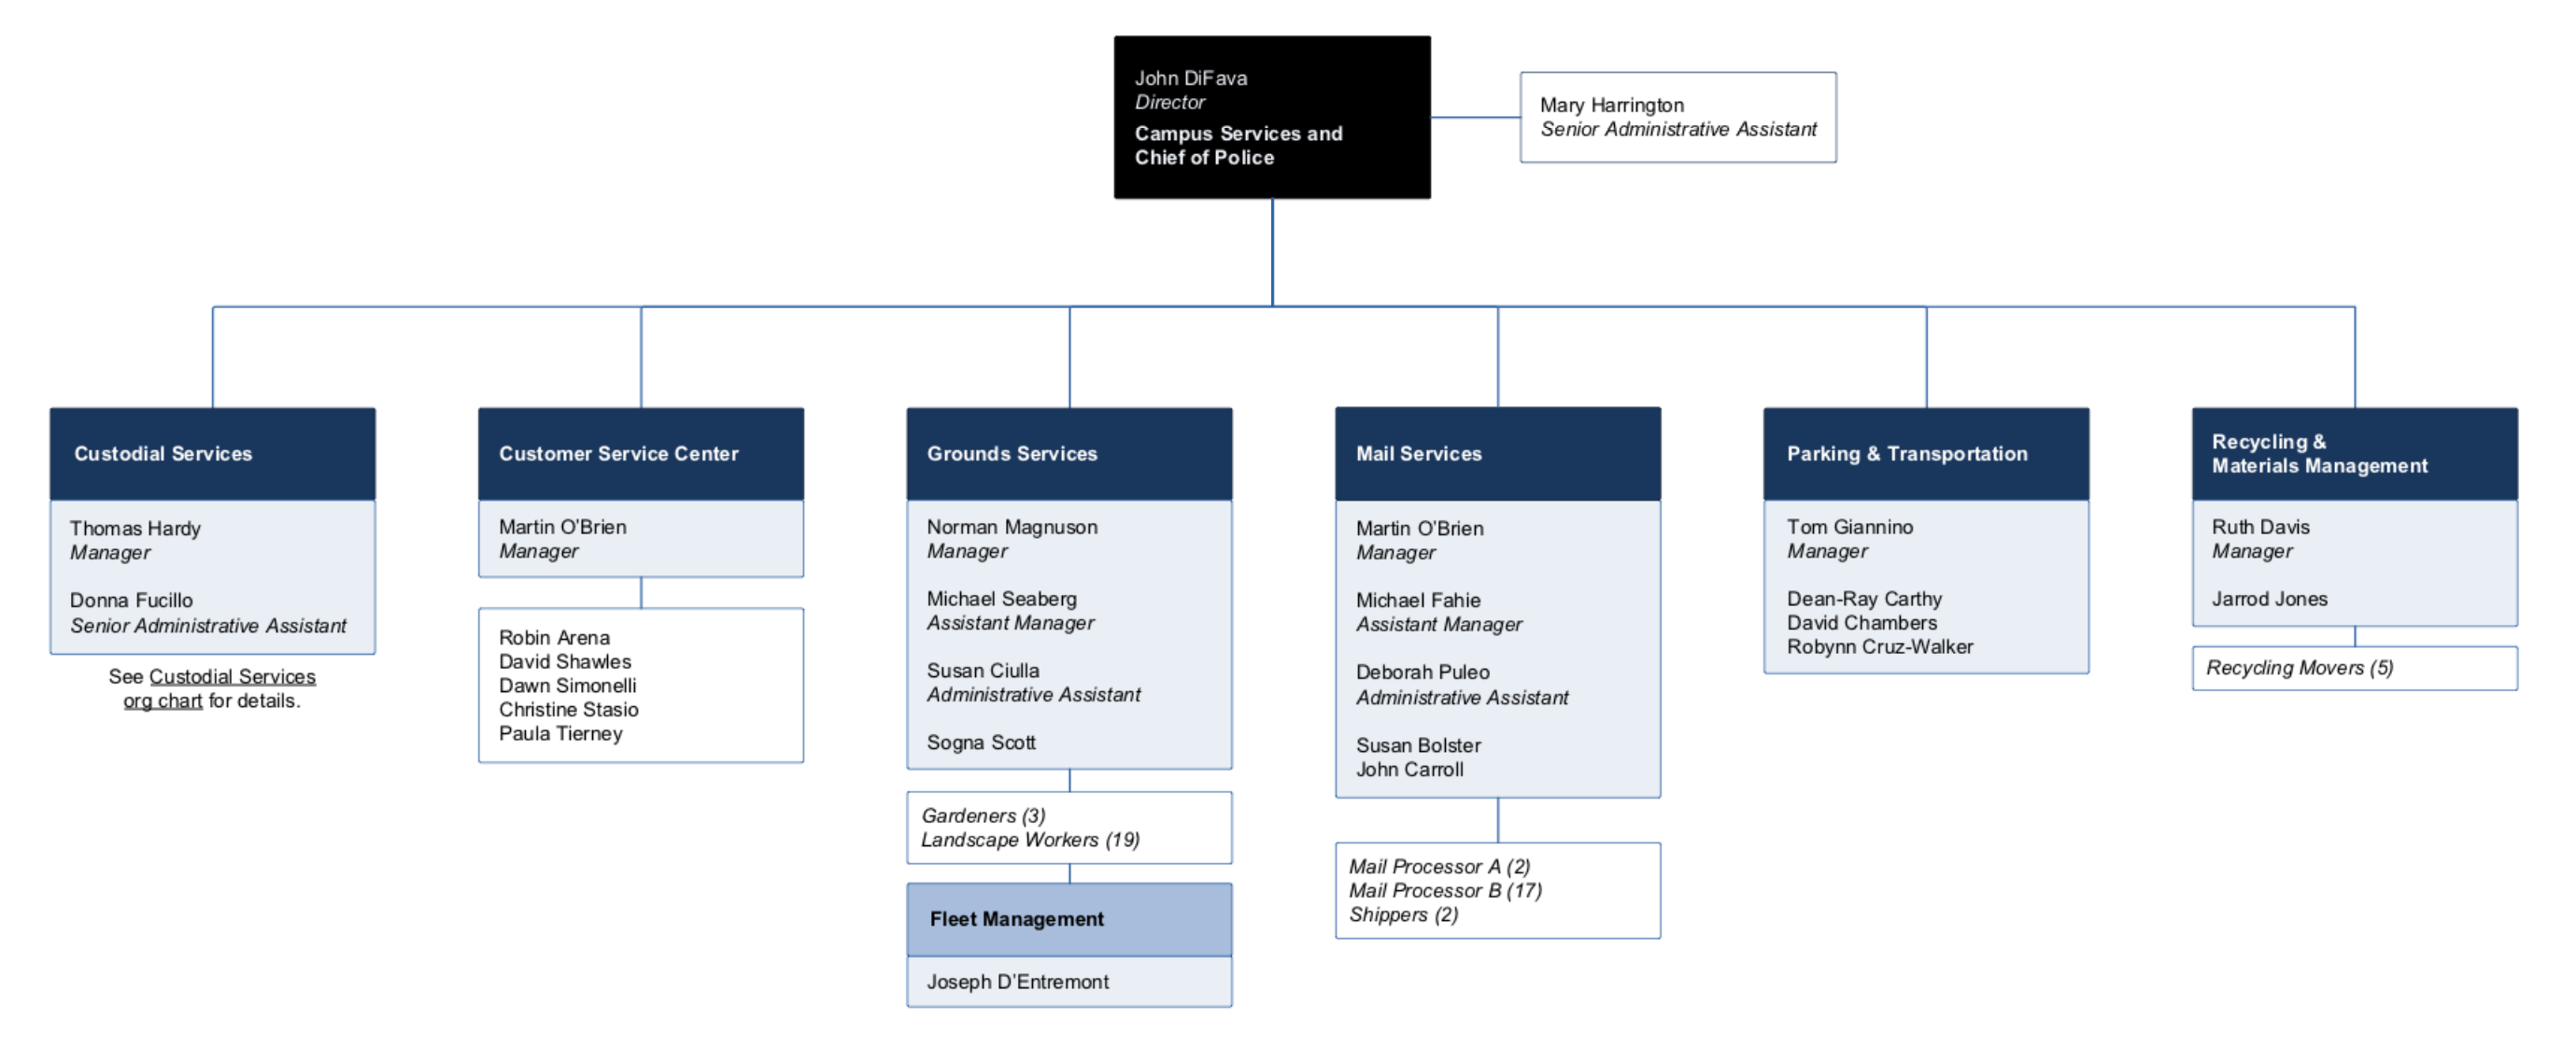
\includegraphics[width=1\linewidth]{img/2/campus-services-overview.png}
    \caption{An organisational chart showing an overview of MIT's Campus Services}
\end{figure*}

\begin{figure}
 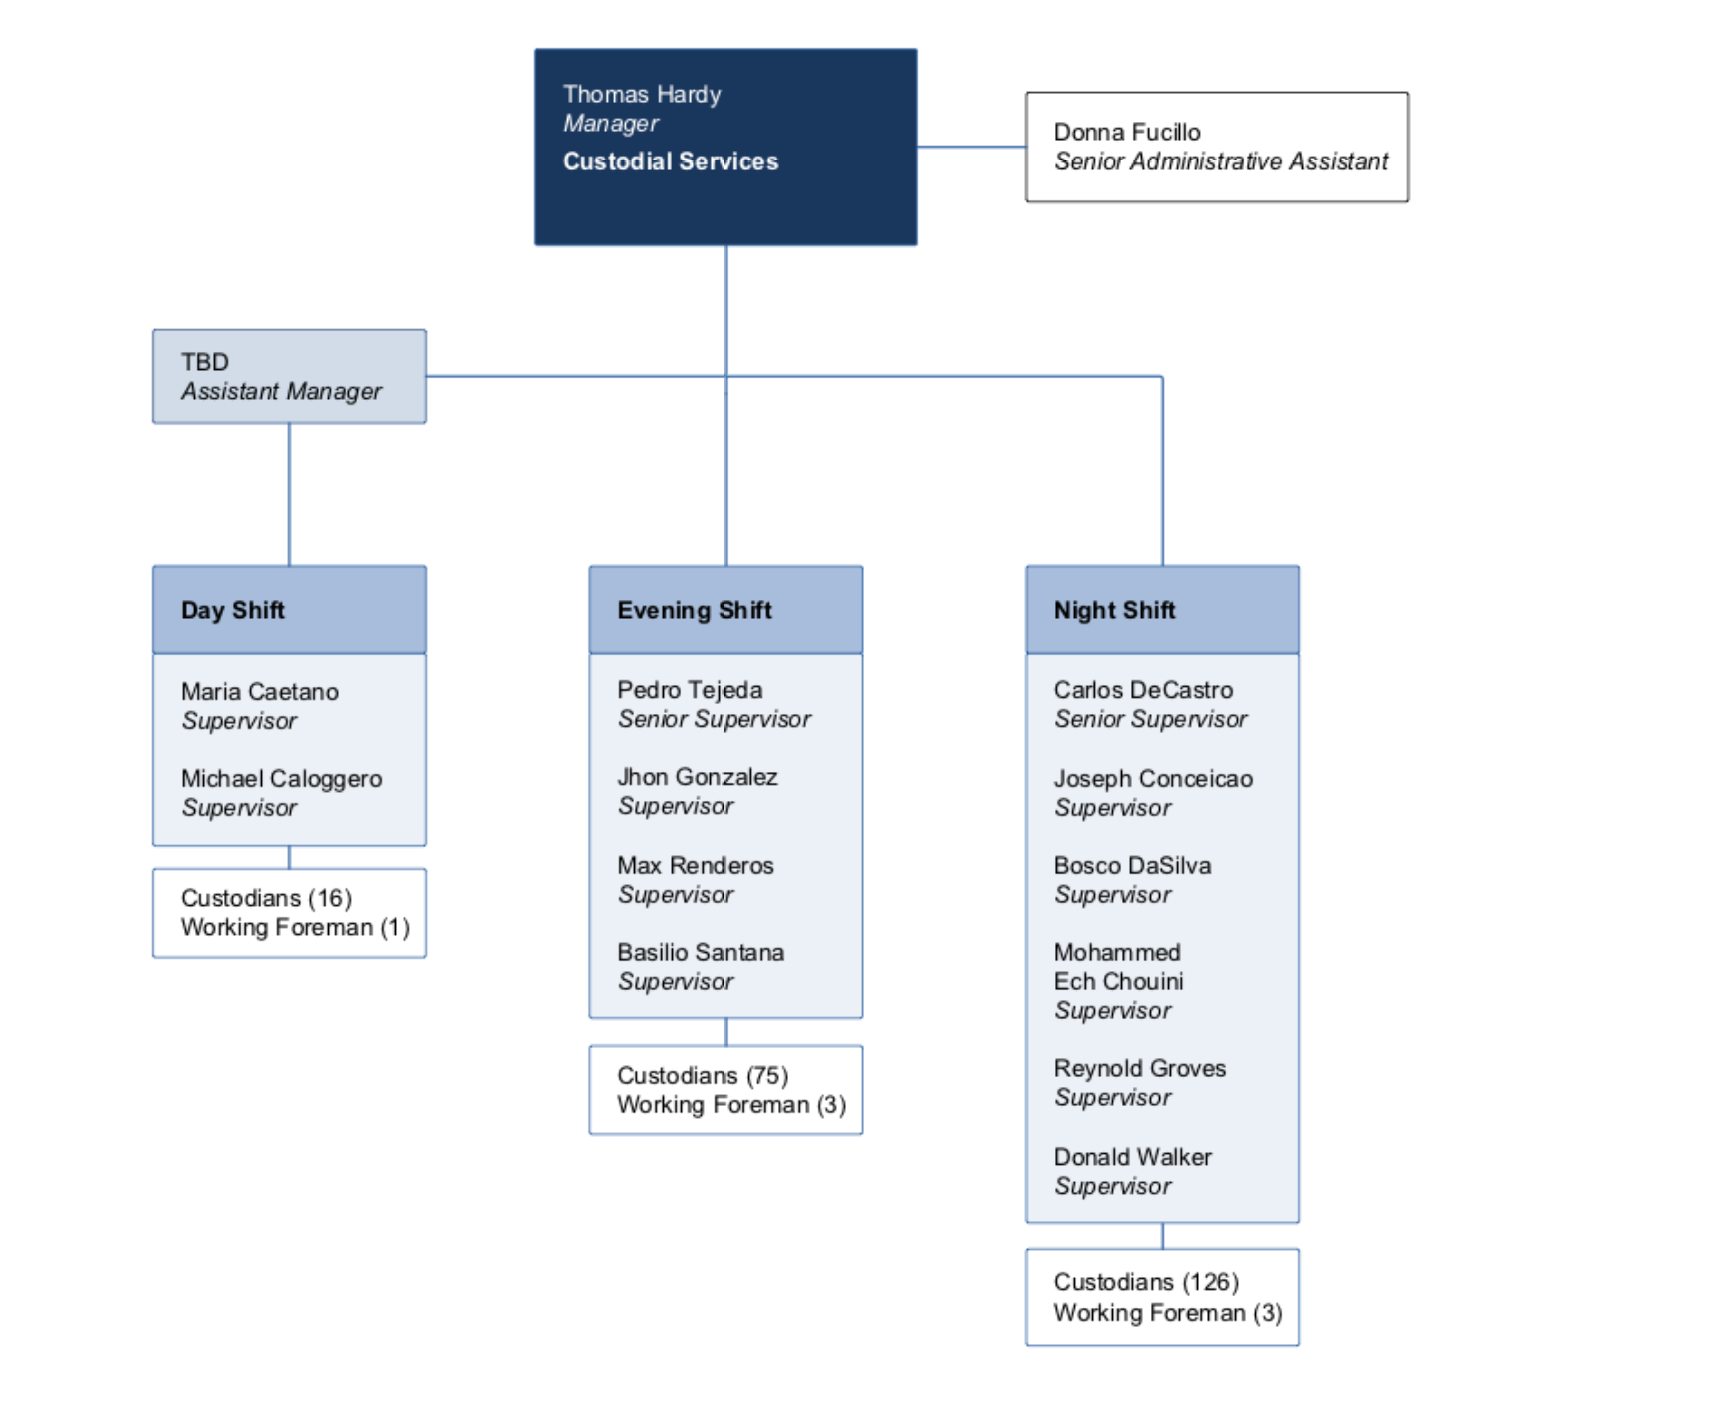
\includegraphics[width=1\linewidth]{img/2/custodial-overview.png}
  \label{orgs}
    \caption{The organisational sub-chart for Custodial Services}
\end{figure}


MIT Office for Sustainability works primarily with the Office of Recycling and Materials Management to collect data about MIT's waste streams and diversion rate from landfill. Currently, the data available online covers landfill waste, recycling, yard waste, food waste, construction and e-waste streams. MIT's current recycling rate has ranged between 44\%-50\% over the past 5 years, though MITOS does not currently collect statistics on recycling contamination rates, which have so far been estimated through one-shot studies (including a waste audit at the Media Lab), and from talking with recycling and custodial staff, who are in charge of spotting and removing contaminated loads. Food waste streams currently comprise only 2.5\% of the materials collected on campus, in part because the institute does not have dedicated compost facilities available at all locations. These were, until recently, turned into compost, but at present they are digested to create biofuels. The Media Lab uses a separate stream to deal with food waste, managed by Bootstrap Compost, a Greater Boston service that composts the waste on local farms.

In 2015, the MIT Campus Sustainability Working Group published a set of guidelines to develop a `state-of-the-art sustainable campus'. The Materials and Waste Management section of the report is focussed heavily on sustainable procurement, with numerous specific policies about purchasing. Speciality streams such as e-waste and styrofoam also feature large, along with potentials to broaden and strengthen re-use networks across campus.

\subsection*{Material Flows}

Over the past decade, the Institute has seen a steady year-on-year rise in the number of packages processed by the mail room, a factor thought to significantly impact the volume of material flow into departments like the Media Lab. The Office of Sustainability emphasis subtlety when addressing the Institute's material consumption. As Brian Goldberg (MITOS) puts it: ``we don't want to tell people `don't buy things'... because they just won't do that. Instead, think about the impact, positive and negative, that the things you buy are having''. Shipping a product might negatively impact the environment, but if that product is being used to further good research, it might be a net positive impact.

%unpick this statement -- is this true? how do you know if you're hacing a positive impact?

Rachel Perlman, a student in the Institute for Data, Systems and Society and organiser with MIT's Waste Alliance cites a lack of centralised data on purchasing as a major factor in understanding material flows through the institute. With research groups using separate accounts across multiple platforms to handle purchases, it is hard to make or enforce policy guidelines. In her work, she advocates for a bottom-up approach to understanding waste systems: going first from audits of waste streams, rather than attempting to control for a higher-level approach. \cite{perlman_material_2016}. Perlman uses ecological metaphors such as `urban metabolism' to describe the consumption and production of waste at MIT, and takes a heavily systems-oriented approach in describing possible interventions.


\subsection*{Zero Waste Initiative}

The Zero Waste initiative at MIT is led by the Office for Sustainability in conjunction with the Office for Recycling and Materials Management, Custodial Services, Bootstrap Compost and Enevo waste management. This is a year-long experiment (academic year 2018-19), which will seek -- as a baseline -- to divert 90\% of waste by volume from landfill, directing it instead to recycling and compost. The first stage of this scheme was an audit of the lab's solid waste streams in November 2018, which found that approximately 50\% of the Media Lab's waste is recycled or composted, though within that, around a third of the recycling is contaminated, bringing the total waste diverted from landfill to a much lower 36\% (Goldberg, 2018). By volume, around 25\% of the materials recovered from the recycling during the audit were non-recyclable. In addition, much of the waste ending up in the trash is food waste, which could instead be composted.

One of the main causes of recycling contamination on campus is due to food waste entering the recycling stream, though harder to spot are contaminants such as black plastics, coffee cups, plastic utensils, and styrofoam, items which students and staff are often unsure whether they can be recycled. Currently, contaminants are identified by custodians inspecting bags from the outside; if a bag is seen to contain a contaminant, it is placed straight in landfill.

To address issues of contamination, a 3-month pilot scheme has been conducted between select (and isolated) areas of the lab: the 2nd floor (including offices, the mezzanine level of the workshop, and 2 research groups), and selected office areas of the 4th floor. The aim of this scheme was to examine whether a combination of education (around recycling, composting, and best purchasing practices), and infrastructural change can advance the zero waste goal of the overall scheme. The infrastructural changes proposed by the scheme are to unify and centralise the waste disposal locations for all of the participating offices. 

Thus far, I have been present at pilot meetings since December of this year, and have attended and helped to facilitate the workshops run for participants in the scheme. This thesis project is being conducted in the context of the educational and outreach part of this pilot, though for the sake of establishing a reliable `control', the evaluation of work developed for this thesis also involves groups not directly included in the pilot scheme. Results from both the pilot, and from these separate studies will inform the roll-out of this program to the wider MIT campus. 

\section*{Interviews}

In order to effectively represent and explore waste systems at MIT, I spent the first month of this project conducting a series of formal and informal interviews with stakeholders throughout MIT's waste ecosystem, including students, organisers, custodians, staff and faculty. The interview process was intended to provide a range of perspectives on the structural dynamics, attitudes, challenges and behaviours that influence waste at MIT.

Each interview centered around 5 questions, chosen to help characterise different perspectives on MIT's waste system, based on the variables identified by Offenhuber \cite{offenhuber_waste_2017}.

\begin{enumerate}
\item What do you see as the biggest structural (financial, spatial, etc) barrier to managing waste at MIT?
\item What do you see as the biggest social (behavioural, attitudinal) barrier to managing waste at MIT?
\item What can individuals do to improve waste management at MIT?
\item What is a change you have seen in MIT's waste in recent years?
\item What do you see as a repeated issue in MIT's waste management?
\end{enumerate}

In particular, I was interested in perspectives not just represented by emails and newsletters -- people that deal directly with waste management at the institute. Across the interviews I conducted, there were a number of repeating themes that operated at both local and global scales.

\begin{figure}
  \caption{A diagram of key interviewees for this project, and their relative affiliations. All actors directly involved in implementing the Media Lab Zero Waste Pilot are highlighted in yellow. This diagram does not include student interviewees}
  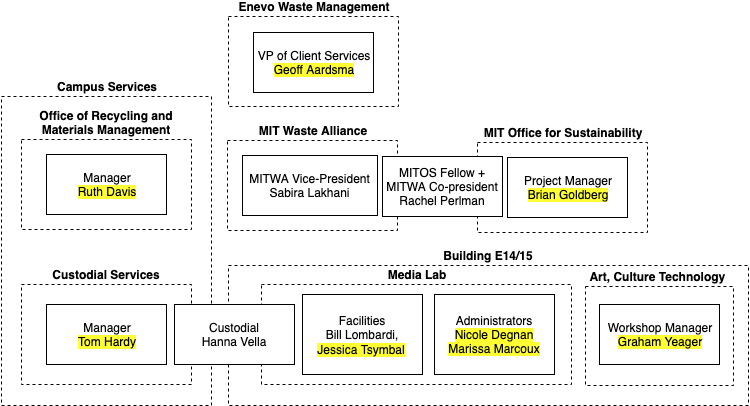
\includegraphics[width=1\linewidth]{img/2/interviewees.png}
\end{figure}

\subsection*{Media Lab-specific}

Problems with waste management specific to the Media Lab come from 2 main stressors. The first is space: despite being a relatively recent development, the lab does not have a good spatial layout for waste disposal, with the loading dock coming up multiple times as a site of frustration. One major issue is that the large recycling bins at the loading dock (intended to take all the recycling collected by the custodians), are also filled with random waste (some recyclable, some not), from building occupants who need somewhere to leave it. With no space on site to clean the bins, loose non-recyclable waste can build up in the bottom, with neither Custodial Staff nor Recycling Staff having any clear remit to remove it.

\begin{marginfigure}
  \includegraphics[width=1\linewidth]{img/2/mit-bins/loading4.JPG}
  \caption{The large blue recycling bins in the loading dock}
\end{marginfigure}

With a couple of exceptions, there are also no clearly visible, centralised locations for waste disposal, meaning that waste streams such as compost (only available in centralised locations), can be under-used. In general, the use of individual bins in offices has been identified as a cause of lower-quality recycling (and lower rates of recycling) across the lab, as the lack of clear and unified signage (and lack of co-location of trash, recycling and compost bins) means that waste is often placed in whatever bin is nearest. This lack of space also factors into the rodent problem in the building. There is no real communal eating space in the lab (though this has improved lately with the increased furniture in the atrium), which means that students often eat in their offices. This is both far from a compost bin (which results in food waste landing in either landfill or recycling), and also means that food waste gets spread throughout the building, making it a friendly environment for mice.

\begin{marginfigure}
  \includegraphics[width=1\linewidth]{img/2/mit-bins/loading6.JPG}
  \caption{Waste piled up in the Media Lab's loading dock}
\end{marginfigure}

The second major factor is the frequency of large events run by external parties in the building. The 6th floor of the Media Lab is administrated not by the lab, but by MIT: this means that external events take place there several times a week, with a large variation in the catering and events management companies used. Unfamiliar with the proper disposal of waste in the lab, there have been multiple occasions where food waste is collected but then not placed in the compost stream, instead sitting (sometimes loose) in the loading dock. The building facilities manager estimated that, during a 2-week period in the summer where the space does not get used, the rodent population in the building halves. In addition, the high number of people circulating the building who are not based there make it harder to establish standards for waste streams in public spaces.

In addition, many people in the lab feel that the building has a very low rate of re-use, with the waste streams at the loading dock consistently filled with perfectly serviceable components (e.g. Monitors, HDMI cables), that are disposed of rather than being pooled within the building. Again, a lack of shared storage space contributes to this issue, and a lack of time (e.g. To ask if anyone needs the items). 

The lab does have a robust internal system for managing food waste (though this has also been linked to the rodent problem). The FoodCam (http://foodcam.media.mit.edu/view/view.shtml) is a webcam that has run, on-and-off, since 1999: when there is leftover food in the lab (e.g. from a meeting or event), it is placed underneath the webcam and a button is pressed, sending an email notification to members of the lab.

\subsection*{Institute-specific}

In general, people I spoke to across both recycling and custodial services felt over-stretched. In particular, with only 5 recycling-moving staff and 2 vans to cover the whole campus, the Office for Recycling has very little flexibility to accommodate an increased workload. Custodial staff are tasked not only with collecting landfill waste, food waste and recycling, and identifying potentially contaminated loads, but also with cleaning the buildings, putting a strict limit on the amount of time that can be dedicated to waste collection and inspection. Although the departments try where they can to co-operate with one another, issues such as the leftover waste at the bottom of the Media Lab bins are common disconnects across campus, where neither party has time to deal with a local issue. Both custodial services staff and recycling staff also identify a lack of breaking down cardboard boxes as a campus-wide issue which consumes a great deal of time and effort.


\begin{marginfigure}
  \includegraphics[width=1\linewidth]{img/2/mit-bins/loading1.JPG}
  \caption{Cardboard accumulating in the Media Lab loading dock}
\end{marginfigure}


Levels of recycling contamination are high across campus, particularly in areas where food is sold, that result in food, food containers and disposable cutlery contaminating the streams. The problem is compounded at sites with both a recycling compactor and food waste present, as it is not possible for recycling staff to separate and examine a potentially contaminated load before taking it to the MRF. If contaminants are found in the compacted load, the whole thing must be disposed of (whereas when the load is still in bins, it is only the bin that is thrown out).

High levels of purchasing from Amazon without much oversight or institutional control was also mentioned several times as an issue, with disconnects in purchasing between (and even within) departments leading to, for example, multiple offices within the same building getting separate shipments of supplies where a single bulk order would do. Amazon packages present a particular frustration, as often these are not broken down and instead left next to bins, creating more work for already stretched custodial staff. This reflects a shift from more centralised control over materials -- where lab managers and administrators would be in charge of the bulk of purchasing -- to a more distributed one, where many students are also trusted with purchasing for their groups. This shift means that individuals are now considerably more responisble for the Institute's material flows than before.

%shift from centralised decisions to individual behaviours

The management of lab waste streams was also highlighted as a particularly serious campus-wide problem at present, as it is not currently possible to recycle pipette tips, lab glass, and latex gloves, all of which are heavily-used disposable items across MIT's labs. In addition, the lack of communication between labs across was identified as a key issue with the re-use and sharing of particular chemicals, with multiple labs found to be buying and disposing of many of the same materials. 


\subsection*{Global}

Some of the issues affecting MIT's waste streams are global, with national and international economic factors playing a constantly-shifting role in the recycling system at MIT. What can and can't be recycled changes all the time, making it very difficult for the institute to maintain consistent signage and education. Even if a talk or a workshop is entirely effective, the information will change in a couple of months: and even recycling right, there's little guarantee that the load will actually be made into new products. China's National Sword program (and subsequent changes to the quality of waste accepted at Casella) was mentioned multiple times.

Composting providers were also an issue, with changing and confusing standards of what should be composted. Municipal composting facilities in Massachusetts cannot process many `compostable' items (such as corn plastics), leading to a great deal of confusion in both purchasing and disposal. 

Across many of the interviews, there was a strong awareness that many of the factors affecting how people waste are deeply infrastructural, emphasising the need for consistent signage, and for waste disposal to be centralised and legible. However, there was also a common frustration that, even in places where this is the case (for example, the campus Student Center), the overall quality of the waste streams is poor, with high rates of recycling contamination (and significantly higher in places where food is served). When asked about the potential reasons for this discrepancy, a distinction was made between a lack of education (leading people to recycle objects such as coffee cups and plastic bags, which they believe to be recyclable), and a lack of care (responsible for `obvious' contaminants of food). The latter was perceived as related both to other stressors (e.g. Work stress distracting from thought about waste practices), and a lack of thought about or engagement with the people responsible for dealing with waste at MIT.

\subsection*{Student Attitudes}

In gauging attitudes amongst students toward waste systems, I conducted a number of informal conversations with graduate students from within the Lab (and from other groups within the building) about attitudes towards waste. These sought to establish the percieved factors preventing students from participating effectively in recycling, and their responses to existing infrastructure, and potential infrastructure change.

In general, students that I spoke to were motivated to waste more sustainably, and everyone reported attempting to recycle and compost where possible. However, most conversations also marked a set of confusions and frustrations around solid waste at MIT, in contrast to domestic waste, which they felt they had more agency over. Common issues were contradictory or confusing signage, lack of access to compost bins (and confusion as to whether the container was for `compostables' or `food waste'), and changing statements about what items are or are not recyclable.

Other factors that limited recycling and composting were the relative distances to various bins. Students who had a trash bin in their office reported rarely walking all the way to a central location to dispose of food waste, because of the relative time and convenience.

In addition, many students were disappointed that not as many of the items that they imagined were recyclable actually were (coffee cups is a prime example of this), and more disappointed that even `good' recycling (e.g. low contamination) could still placed in landfill at high rates. Multiple students expressed their frustrations that they had seen custodial staff placing recycling bags in the trash, and were not aware that this might be due to recycling contamination rather than simple carelessness. In some cases, students said that these frustrations, combined with other distractions, lead to them `giving up' trying to waste well. This sentiment correlates with the `lack of care' toward the system perceived by waste management staff.

%much deeper synthesis: how much should a representation challenge the status quo?
If a part of this study is tackling recycling contamination, another part must also address the extent to which recycling is inadequate for dealing with a large amount of the waste that we produce, and highlight routes for productive participation in campus waste streams.

\begin{figure}
\includegraphics[width=\textwidth]{img/2/signs-collage.jpg}
\caption{A large variation in signage within the media lab, often with conflicting imagery, layout and information}
\end{figure}



\chapter{Playing With Trash}

\section*{Proposal}
Based on this picture of waste systems at MIT, I propose that there is a relationship between the attitudes and ideas that students have about waste infrastructure at MIT, and the resultant quality of the waste produced. In addition, I posit that making legible the broader context of waste systems within and around MIT (rather than just the specifics of what one should and should not recycle) is an important part of educational interventions, as many of the issues on campus operate across local and global scales.

This thesis builds two civic games that seek to influence the culture of waste management in the Media Lab, and within the wider community. Both specifically address the identified issues of recycling contamination and unsustainable purchasing, while seeking also to shape the collective imaginary of waste systems, and address broader issues of infrastructural legibility. 

Throughout, the aim is to emphasise:

\begin{enumerate}
\item complex and counter-intuitive aspects of municipal waste systems
\item the relationship between the player and the waste system
\item the potential for action (both personal and infrastructural) within the waste system
\end{enumerate}

\subsection*{Aims}

A key aim within realising these goals is to encourage positive behaviours toward waste, and tackle the hopelessness and frustration felt by students when dealing with changes in recycling infrastructure. These games are intended to act as educational tools that accompany infrastructural change, acting as both an explanation and a motivator.

\subsection*{Timeline}

The timeline for the Zero Waste Pilot study is between February-April 2019. Over this period, the waste infrastructure the pilot locations is changed to a centralised layout with clear signage, and all participants are invited to a series of workshops: one at the start (February 4th), one at the midpoint (March 13th), and one at the end of the study (). These workshops are for both educational and feedback purposes, and involve staff from all parties involved in the pilot scheme, in addition to student organisers from the MIT Waste Alliance.

\section*{Trash Poker}

The first component of this project is a design for a card game, that develops on the basic model of the `recycling classification' game to create a more complex scenario where players compete to contaminate one anothers waste streams. This game was developed for the initial workshop of the Zero Waste Pilot scheme, and was intended as a complement to talks on Institute recycling from Ruth Davis, and Brian Goldberg.

%ADD: Re-inforce knowledge of reycling practices but also generate a critical conversation around waste. not just sorting but also thinking about effects of contamination. Doesn't just improve a skill but uses critical perspective

The idea for the game first came after a conversation with MIT Learning Arcade's Scot Osterweil, about the idea of Virtuous Player Syndrome. Virtuous Player Syndrome is a term he uses to describe civic games where you win by performing the `correct' action and behaviour to get through the game as quickly as possible. Instead, he argues that games where the player must perform transgressive or morally ambiguous behaviours to succeed gives rise to a greater level of reflection \cite{osterweil_civic_2011}. Thus, instead of simply sorting recycling, players are required to make strategic trade-offs: do you contaminate a player's waste stream with food waste, or do you wait to see if you can steal their compost bin? Are coffee cups recyclable, or are you handing them points?

The goal of this game is to increase and consolidate specific knowledge about the waste stream that each item should be placed in, as well as highlight the importance of speciality streams in dealing with the complex waste produced in the lab.

\begin{figure}
  \caption{A selection of the \emph{Trash Poker} cards}
  \includegraphics[width=1\linewidth]{img/3/trashpoker.png}
  \label{contamination}
\end{figure}

\subsection*{Overview}

The game is played in pairs. Each pair starts the game with their own recycling bin, containing 12 items (one of each item), dealt face up. Pairs are also dealt 3 instruction cards in their hand, face down. 

In the middle of the space is a trash bin where unwanted items are discarded. There are also special bins that appear during the course of play. 
The goal of the game is have the most recyclable items in your recycle bin and any specialty bins (e.g. compost, clothing) you might also have, whilst avoiding contaminating these bins with items that shouldn't be there. 

Play proceeds in turn. Each pair chooses a new instruction card for their hand, adds it to three that they already have, and publicly plays one, following its instructions. At the end of their turn, the pair may place one item in the trash, or in a speciality bin (if owned), in addition to whatever items may have been played during the turn. 
Play ends when the deck of instruction cards is depleted. For each correctly-placed item in the recycling bin, or in a speciality bin score +1 point. For each incorrect item, score -1 point. For reference, at the end of the game, the rule-sheet may be turned over: this has the correct labelling of items. 


\subsection*{Development}

The game was developed over a 2-week period, during which time it went through 2 rounds of iterative play-testing, which shaped the eventual rules. In-between each round, feedback was incorporated to refine the game.

\subsubsection*{Playtest 1:}
This play-test mostly weeded out dull and unhelpful cards, and helped to develop the rules of the game. Initially, players had too few opportunities to discard items from their recycling bin, and so adding in a turn-wise trashing step helped to move the game along. The speciality streams proved to be one of the more interesting mechanics, but their role needed to be clarified, as they added some complexity to the rules. In general, most comments related to improving the legibility and balance of the game.

\subsubsection*{Playtest 2:}
The second play-test took place in a meeting of the Viral Communications group, and included 15 players, 10 of whom played in pairs. In this iteration, the rules proved somewhat easier to understand, and were condensed into a final version during the meeting (thanks Andy!).
The most specific feedback from the gameplay was that the game was too disheartening: with most of the items available not recyclable, it was hard to get a positive score, and left players with the feeling of futility. There were also too many items, requiring a lot of time at the start of the game to deal the right number to each player, and confusion as to slight differences between some of the cards (e.g. Multiple plastic bottle cards). To correct this, the number of items was condensed to just 12: 4 recyclable, 4 trash, and 1 each for every speciality stream (e-waste, clothing, compost, batteries).


\section*{Let's Play, Waste at MIT}

The second component of this project is a digital, single-player simulation game that draws upon critical simulations such as Universal Paperclips and The Founder for inspiration. Players are given administrative control of the MIT campus for which they attempt to earn `zero waste' status by diverting more than 90\% of all waste from landfill. This is achieved by navigating a changing set of internal and external mechanics, which multiply in number and difficulty as the game progresses.

By taking control over the structural dynamics of the waste system while being influenced by the actions of individuals (e.g. you can decide which buildings get cleaned, but a variable you can't control is how individuals recycle), participants learn about the complexity of the waste systems in the institute while reflecting on their own role within them. The goal of this game is to encourage the player to consider themselves as an actor within a broader system of waste, and engage with the effects (both positive and negative) that they can have as part of the community. It also encourages a broader picture of the complexities inherent in managing waste systems, and the real limitations affecting those tasked with managing waste on the MIT Campus.

Where possible, the narrative elements of the game are taken directly from conversations with people involved in waste management on the MIT Campus.

\subsection*{Waste at MIT as a Complex Information System}

In order to develop a systems simulation of waste at MIT, it was necessary to develop a series of system diagrams and models to simulate various aspects of the system. While it is not conceivable to represent all of the variables at work in capturing the waste stream, I attempted to represent, in some manner, all of the key concerns that had arisen as part of the interview process. 

Using Offenhuber's classification of representational elements of waste systems, the variables in the simulation can be divided into 3 main groups:

\subsubsection*{1. Structures and Processes
}
\textbf{Definition:} Spaces, places and infrastructures of waste disposal, and the processes involved in navigating between them.

\noindent\textbf{At MIT:} Buildings, recycling trucks, bins, compactors, food vendors, labs, databases, space (/lack thereof), compost
\subsubsection*{2. Actors and Consequences
}
\textbf{Definition:} Participants in the system, and the consequences of their actions.

\noindent\textbf{At MIT:}
Actors: Students, custodial staff, facilities managers, lab managers, faculty\\
Consequences: contamination, rodents, good/bad purchasing practices
\subsubsection*{3. Governance and the Individual}

\textbf{Definition:} The role of civic initiatives and policy within the management of waste systems.

\noindent\textbf{At MIT:} Funding, staffing, working hours, human resources, resource allocation, choice of recycling style/provider, purchasing, what can/can't be recycled/composted

Throughout development of the game, the player was given control over governance variables in the system, with Structures and Processes forming the most consistent constraints and mechanics in the game, and Actors and Consequences relying more on stochastic processes.

\subsection*{Prototyping Systems}

% Specifically, causal loop diagrams

To prototype the game mechanics, I used a systems simulation tool designed by Nicky Case called Loopy! \cite{case_loopy!_2017}, which allows for the emergent behaviour of multiple different interlinked variables to be modelled. This allowed rapid iteration on different arrangements of variables and starting conditions, and showed some of the possible `end states' of the game. In particular, I was interested in producing compelling and unexpected narratives that would allow a broad space of possible outcomes.

%expand this?
\begin{marginfigure}
\caption{A causal loop diagram of the `adoption' model used to demonstrate systems dynamics, showing interacting feedback loops describing the adoption of new products. As a product is adopted, this increases the word-of-mouth spread of the product, thus increasing the adoption rate. Simultaneously, however, adoption eventually saturates the market, providing negative feedback. \cite{blleininger_english_2010}}
  \includegraphics[width=1\linewidth]{img/3/adoption.png}
  \label{contamination}
\end{marginfigure}

Loopy!, described by Case as a `tool for thinking in systems' uses the block-and-arrow notation of feedback systems to indicate positive and negative relationships between variables. The length of an arrow between two blocks indicates a time delay in feedback, and the size of the circle inside each block indicates the `stable' initial value. The system is then simulated by perturbing one of these variables from this initial stable state (up or down), and observing the resultant emergent behaviour.

\subsection*{Initial Experiments}

\begin{figure*}
  \centering
  \caption{Initial Experiments with \emph{Loopy!}}
  \label{optimising}
\begin{subfigure}{.3\textwidth}
  \centering
  \includegraphics[width=1\linewidth]{img/3/loopy/small-static.png}
\caption{\textit{Initial system, static}}
\end{subfigure}
 \quad
\begin{subfigure}{.3\textwidth}
  \centering
  \includegraphics[width=1\linewidth]{img/3/loopy/small-win.png}
\caption{\textit{Winning the game}}
  \label{small:win}
\end{subfigure}%
\quad
\begin{subfigure}{.3\textwidth}
  \centering
  \includegraphics[width=1\linewidth]{img/3/loopy/small-lose.png}
  \caption{\textit{Losing the game}}
  \label{small:lose}
\end{subfigure}% 
\end{figure*}
\vspace{0.8cm}

The first experiment with Loopy! was to produce a `virtuous closed loop': a simple feedback loop that modelled a fairly simple relationship between recycling budget, bins, staff, and quality. Here, the blocks are colour coded to show external variables (orange), controllable policies (red), behaviours (green), and outcomes (blue). In this case, an initial increase in recycling staff produces the diagram on the far right, where there are large numbers of happy staff, quality is high, and recycling costs are low (yay!). Alternatively, the diagram in the centre shows the result of an initial reduction in staff numbers: death, destruction, and extremely costly recycling. This is obviously a simplistic model, but even tweaking variables during the simulation can produce interesting, dynamic and chaotic behaviours.


\subsection*{The `bigger picture simulation’}
\begin{figure*}
  \centering
  \caption{Developing a more complex approach}
  \label{optimising}
\begin{subfigure}{.3\textwidth}
  \centering
  \includegraphics[width=1\linewidth]{img/3/loopy/big-static.png}
\caption{\textit{Initial system, static}}
\end{subfigure}
 \quad
\begin{subfigure}{.3\textwidth}
  \centering
  \includegraphics[width=1\linewidth]{img/3/loopy/big-win.png}
\caption{\textit{Winning the game}}
  \label{small:win}
\end{subfigure}%
\quad
\begin{subfigure}{.3\textwidth}
  \centering
  \includegraphics[width=1\linewidth]{img/3/loopy/big-lose.png}
  \caption{\textit{Losing the game}}
  \label{small:lose}
\end{subfigure}% 
\end{figure*}
\vspace{0.8cm}

The next model created incorporated a much larger number of variables, to better describe the interactions between the waste system and campus as a whole. Incorporating ideas from the interviews such as space and stress, and a comparison between landfill waste and recycling. By playing with feedback dynamics (such as the delay between hiring new staff, and having to pay them, and the effects of the space on stress), a more complex simulation is achieved. However, there are still issues of `virtuous player syndrome' -- the simulation still succeeds if you install enough staff.

%expand this?
\begin{marginfigure}
  \caption{Jay Forrester's `World Model' simulated using a causal loop diagram in \emph{Vensim} \cite{noauthor_vensim_nodate}}
  \includegraphics[width=1\linewidth]{img/3/vensim.png}
  \label{contamination}
\end{marginfigure}

\subsection*{Reaching the limits of Loopy!}

As this development of the game progressed, Loopy! became less useful to account for more specific, nonlinear relationships between variables. For example, set monthly budgets limit the number of staff you can add, and make trade-offs with other variables in the simulation. A tool that might be better suited to this stage in future projects is complex systems simulation tool \emph{Vensim}, industrial systems-modelling software that is free for educational use (but otherwise requires a license). 

\begin{marginfigure}
  \caption{An agent-based network model in a preview of Francis Tseng's \emph{syd} \cite{tseng_big_2016}}
  \includegraphics[width=1\linewidth]{img/3/syd.png}
  \label{contamination}
\end{marginfigure}

Francis Tseng's \emph{syd} (short for `system designer') might provide a more accessible and open-source alternative to \emph{Vensim}: currently under development, it incorporates the causal loop diagram with more complex agent-based and network models \cite{tseng_big_2016}. 

\subsection*{Narrative Aspects}

In order to give the game a narrative form, the player speaks to several characters from around campus throughout play, the dialog with whom is based on conversations had during the interview stages of the project.

Players manage variables including the hiring and training of custodial staff, investment in different forms of waste disposal, different education and waste tactics and budget. Factors affecting the players include rates of recycling contamination, the consumption of different kinds of products, relations between different waste management teams and the proliferation of rodents.

The key task here is to relate the `systems problems' described by the model to interesting decisions and trade-offs within the game. In his Criteria for Strategy Game Design, Fabian Fischer \cite{fischer_criteria_2014} puts forward a theory of the `interesting decision' that sits between a guess and a solution, as an ambiguous problem with a set of consequences. Interesting decisions are achieved by balancing the amount of information given to the player at a time: enough that the decision is not simply a guess, but not so much that the consequences of the decision are obvious.

In addition, care was taken to make the game sensitive and responsive to the needs of the custodial staff. Complaints of staff in the real world (too many bins, too few staff, too many rodents), and more general management practices (hiring/firing, training), contribute to a `staff happiness' index, shown to the player both as a discrete indicator (and emoji), and elucidated through dialogues with characters. This index proves a major factor in the game dynamics, with staff striking if it falls below a certain level, and the player themselves getting fired if the score is consitently poor.

The `efficiency' of the game is also important: the amount of time a player spends making interesting decisions, vs waiting or performing tasks that have few consequences for the gameplay. Game designer Keith Burgun argues that efficiency in this sense should be maximised: ``If players give you five minutes, that's a huge gift and you owe it to them to make sure it is completely rewarded''. Transparency of the game mechanics are also important: an awareness of how the current state of the game came about, the alternative courses of action that could be taken, and some idea of immediate consequences of those actions. 

\subsection*{Playtesting}

The game development took an iterative cycle, at each stage being critiqued by a different group to evaluate its playability, quality, and educational aspects. At each stage, I was seeking to answer a different question: is the game playable? Is the game compelling/well-designed? 

\subsubsection*{Students I}

In the initial stages of development, I conducted regular informal play-tests with friends from within the Viral Communications group (thanks in particular to Kalli and Oceane). At the start of the game's development, these mostly served as good crash-tests for elements of the interface and mechanics, and a lot of bugs were discovered this way.

Initial feedback related heavily to the game's transparency: what different statistics mean, what the goals of the game are, and what the immediate result of particular actions are. In order to make the game more strategic, pausing the gameplay while choosing various courses of action became important. This relates back to questions of infrastructural legibility in the first place: how can a game communicate a system when its own internal logic remains opaque?

After these comments, I introduced a set of charts to the interface to see the impact of decisions over time, and allowed the game to pause. I also added increasing levels of difficulty as the game progressed, to introduce new goals and mechanics gradually, rather than all at once.

\subsubsection*{Game-Lab Researchers}

During the end of the prototyping phase, I organised a formal play-test with a group of four researchers from the MIT Game Lab (thanks to Rik Eberhart, Philip Tan, Sara Verrilli and Jan Mikael Jakobsson), in order to get feedback on the quality of the game. They played the game in pairs, with mixed results: one pair managed to get the recycling programme running well and divert a significant amount of waste from landfill, while the other was rapidly overcome with rodents.

%how did this shape an experience of it? would pair-playing change a perception

We had a long discussion afterwards about the game's qualities, and the relative merits of different strategies and techniques. In particular, the transparency of the game needed development, and the relationship between the representational elements of the game and the calculations performed was also a point where the game didn't quite work. (e.g. The game can give the impression that changes take place on the building level, whereas most calculations consider the campus as a whole). In general, they thought the game was engaging -- perhaps too much so to get the point across -- comparing the mechanic to a `spinning-plates' rather than a strategic game.

After these comments, I made an effort to make feedback to the player much more transparent, and added explainers to all of the options that a player might be presented with during the game. 

\subsubsection*{Students II}

At this point, the game was fully playable, and I sent it to a larger number of peers to test. Reviews were generally positive, with all respondents saying that they felt they had learned something, and that they thought more deeply about the people who managed their waste. Nobody had been able to win, however, with even the most successful players running drastically over-budget at the end of the game. Other comments were greater specificity in the narrative. Interestingly, this reflected other student complaints that I'd heard of the language used around waste management on campus: too many different and ambiguous words!

\subsubsection*{MIT Waste Management}
Feedback from people within MIT's waste management was positive, with most respondents finding the game to be compelling, and an accurate representation of how managing municipal waste can feel.

Brian Goldberg (project manager at MITOS), stated: ``I do believe that if more people play this game, they’ll better appreciate the challenges that a campus faces in managing these issues'', citing the difficulty of the game, and the many different variables involved, as being aspects that address the difficulties of managing the waste system.

Aspects to improve were to have clearer visuals (e.g. a student emoji instead of students), and more transparent feedback, as this would aid decision-making in the game, and limit confusion.

\subsection*{Development}

\begin{marginfigure}
\includegraphics[width=\textwidth]{img/3/prototyping/early-day.png}
\includegraphics[width=\textwidth]{img/3/prototyping/early-map.png}
\caption{Stills from the command line simulation, showing gameplay, and an overview of the campus }
\end{marginfigure}


Let's Play: Waste at MIT was developed as a series of prototypes between December 2018 and April 2019. The initial iteration used a command-line interface written in NodeJS for the sake of fast prototyping without the need for detailed graphics, using ascii representations to interface to the backend. This allowed for the development and demonstration of basic game mechanics, but quickly grew unwieldy when dealing with multiple menus and asynchrony. Due to issues of accessibility and sharing over the web, this was never intended as the final iteration.

The next version used a combination of Javascript and JQuery to compose a web interface. This was an improvement in user experience, using a single page view of the game to interface with menus, maps and statistics. However, after a couple of weeks' development the number of asynchronously updating components on the page had started to cause issues with complexity, and the choice of language made it difficult to write structured, legible code.

\begin{marginfigure}
\includegraphics[width=\textwidth]{img/3/prototyping/initial-map.png}
\caption{An initial version of the Javascript and JQuery interface, which was re-created and improved in React }
\end{marginfigure}

The third and final iteration of the game used the React JS framework to manage the single-page interface. This allowed the interface to be broken down into a series of structured components, which could be rendered asynchronously, and allowed for the use of Redux Stores, a means of persisting the client state after the page is closed and reloaded. In order to properly balance the game mechanics, an economic simulation was built in Excel, and then translated into the game environment.

The interface is comprised of a series of structured components. \verb|Stats.js| handles the rendering of the statistics bar at the top of the interface, and also contains the timing component which forms the core of the simulation. \verb|GameMap.js| handles the rendering of the map in the centre of the page, including buildings, characters and their thoughts. \verb|Sidebar.js| renders a second set of statistics at the side of the page. \verb|Menus.js| handles the rendering of menus, which change as the game progresses. \verb|Scripts.js| renders interactions with the game's characters, and drives the main narrative element of the game.

A set of `helper' files contain constants and helper functions, and do not relate to particular sections of the interface. \verb|economics.js| is where the bulk of the backend calculations that drive the simulation are located. \verb|characters.js|, \verb|buildings.js|, \verb|menus.js|, \verb|constants.js|. store information about characters, buildings menus and numerical constants respectively.

\subsection*{Overview of Final Design}
After around a month of iteration, modelling and playtesting, a final version of the game emerged. A systems diagram of the gameplay is shown below: similar to Loopy!, it uses the `feedback loop' as a core motif, but now incorporates thresholds, events and other variables.

\begin{figure*}
  \includegraphics[width=1\linewidth]{img/3/mitwaste.png}
\caption{\textit{The game system diagram}}
\end{figure*}

\begin{figure*}
  % \centering
  \shadowimage[width=0.8\linewidth]{img/3/gameplay/l1.png}
\caption{\textit{1. Beginning the game}}
\end{figure*}
\begin{figure*}
  % \centering
  \shadowimage[width=0.8\linewidth]{img/3/gameplay/l2.png}
\caption{\textit{2. Managing the recycling rate}}
\end{figure*}%
\begin{figure*}
  % \centering
  \shadowimage[width=0.8\linewidth]{img/3/gameplay/l3.png}
\caption{\textit{3. Dealing with recycling quality and contamination}}
\end{figure*}
\begin{figure*}
  % \centering
  \shadowimage[width=0.8\linewidth]{img/3/gameplay/l4.png}
\caption{\textit{4. Implementing speciality streams}}
\end{figure*}
\begin{figure*}
  % \centering
  \shadowimage[width=0.8\linewidth]{img/3/gameplay/l5.png}
\caption{\textit{5. Tackling purchasing issues}}
\end{figure*}%


\chapter{Evaluation}

\section*{Study Design}

In this section, I review methods of evaluation for civic games, and techniques for collecting attitudinal and behavioural data about waste streams. I then introduce a 3-week, mixed-methods study of the simulation game, and discuss its design. I then outline a similar study of the recycling card game, and describe a second, less-formal analysis which discusses the effectiveness of the card game in the context of the pilot workshops. %I then describe a further two studies using less formal methods, the first of which uses an online audience to evaluate the general potential of the simulation game, and the second which discusses the effectiveness of the card game in the context of the pilot workshops.

\subsection*{Evaluating Civic Games}

Evaluation methods for Civic (Serious) games have been the subject of much debate over the past decades, with Mayer et. Al's 2014 survey of approaches providing one of the most comprehensive recent frameworks for evaluation. They describe a conceptual framework for serious games research that takes into account both individual and structural dynamics, and providing detailed examples of evaluation methods in the context of larger systems at play (see ifg \ref{mayer}) \cite{mayer_research_2014}. In particular they focus on the use of Civic Games as a way to develop complex knowledge, and civic skills.

\begin{figure}
  \caption{Mayer et. al's overview of the conceptual framework surrounding civic gameplay \cite{mayer_research_2014}}
  \includegraphics[width=1\linewidth]{img/4/mayer-diagram.png}
  \label{mayer}
\end{figure}

They define a set of potential research questions that are typically addressed using Civic Games research, dividing approaches into design-oriented (making it better), intervention-oriented (making it work), domain-oriented (making it matter), and disciplinary research (making it understandable). This instance is both domain-oriented: how effective is gameplay in describing the complexities and nuances of waste at MIT, and intervention oriented: what behaviour or attitude changes are driven by this awareness? Thus, a multi-method reporting approach is used, where a combination of self-evaluation (domain-specific knowledge), open-ended questions (attitudes and domain-awareness), and empirical measurement (behavioural changes), are used to give a picture of the game's effect.


\subsection*{Evaluating the Simulation Game}

Given the time frame of this work, it is not possible to perform a longitudinal study on the effects of the simulation game. However, short-term changes in attitudes and behaviours may be observed through the use of a controlled, localised study. This study will seek to determine:
\begin{enumerate}
\item Does playing the simulation game contribute to a change in attitudes toward waste systems?
\item Does a change in attitudes correlate to a change in behaviours?
\end{enumerate}

In order to evaluate both of these questions, a concurrent mixed-methods approach is used. Mixed-methods research combines both qualitative and quantitative techniques as a means of both triangulating particular conclusions drawn from the data, and to broaden the scope of enquiry. In their survey of Game-Based Learning evaluation techniques, Mayer et. Al posit that all serious games evaluations should incorporate a mixed-methods approach, due to a combination of related empirical and affective data generated before, during and after gameplay \cite{mayer_research_2014}. `Concurrent' indicates that both data types will be collected simultaneously.

This study comprises two main components. The first component is a survey, which participants take before and after playing the game. This uses a combination of qualitative and quantitative questions to evaluate the change in both the player's understanding of waste systems, and their attitudes toward waste. The second component is a quantitative test of behaviour change, collected through repeated randomised analysis of office recycling streams related to the player over the course of a 3-week period.

The population for this study are students within the Media Lab. These students are selected based on location, with participants solicited in groups related to a particular area of the lab. This selection allows for the isolation of waste streams required for the second part of the study. The survey measures change in attitudes and understanding (rather than absolute values), in order to incorporate populations with differing initial views and education levels on issues relating to waste.

\subsection*{Survey design}

The survey component aims to address the research question in 2 key ways:

\begin{enumerate}
\item Has playing the game increased the participant's understanding of complex effects in waste systems?
\item Has playing the game changed the attitudes of the participant toward waste systems?
\end{enumerate}

While there are a number of models for campus surveys about recycling available as examples, these tend to focus primarily on peoples' ability to and willingness to recycle, rather than their awareness of recycling as a part of a broader waste system. For more complex examples, I used Lee et. Al's questionnaire from the Tracking Trash project \cite{lee_learning_2014}, and Kevin Lynch's interview questions on Waste and Loss \cite{lynch_wasting_1990}. Lee et. Al use Likert scales to evaluate specific attitudes toward and awareness of waste systems, while Lynch employs open-ended questions that allow the player to express more complex or generalised sentiments toward waste.

%relative merits of approaches and how they influenced

The pre- and post- game survey are similar, save for some questions reserved in the post survey for the player to give feedback and opinions on the game play itself, and some asked of the players at the end of the study (after a couple of weeks). The first part of the survey is evaluated through largely quantitative methods, employing a Likert scale to record a change in how waste is `understood', and the second includes broader Lynch-inspired questions such as `Think about the last time you threw something away? What were you thinking about (if anything) when you did?'. 


\subsection*{Waste audit design}

Waste audits are one of the most effective ways of characterising institutional waste streams, and identifying opportunities for change in waste management practices \cite{smyth_reducing_2010}. As this waste audit is focussed specifically on the behaviour of individuals relative to a waste stream (rather than the impact of contaminants in general), this study analyses the percentage of contaminants `by action' rather than by weight or volume (as is normally the case for waste audits).

Hence, measurements are taken of the ‘number of contaminants as a proportion of the number of items recycled’. This involved some estimation: for example, one sheet of paper might be an individual ‘recycled’ object, but if a sheet appears as part of a larger document (e.g. obviously related to other pages), or folded with other pieces, it should counted as a single recycling event. 


%Please show what you controlled for and how.  Then you can note elements you could not control for.

% \subsection*{Online Study}

% The second study of the simulation game uses a concatenated version of the survey to assess changes in attitude and behaviours, and does not include a waste audit. The population for this study are members of the general public, who take part in the game via the internet. This population has a potentially higher degree of randomness, though depending on the channels of distribution (e.g. Media Lab accounts) the population reached is unlikely to be fully randomised. Participants in the online version of the game will be given the option to complete component (1) before and after play, with only those who have completed the pre-game survey permitted to take part in the post-game survey.


\section*{Simulation Game Study}
This study was conducted in the Media Lab, with the Object Based Media Group. This group was chosen as their office space is not shared with any other groups, and they are located away from the main thoroughfares of the building. Out of 11 total current members of the group, 8 participated in the study.

Participants were informed when consenting to take part in the study that a waste audit would be performed on random days in the lab. Participation in the main study itself took place over a 2-day period, where members of the group played the online version of the game, and completed surveys 1 and 2. No waste audit data was collected during that time.

This study was generously funded by MIT's Living Labs Initiative, who compensated participants for their time.

\subsection*{Controls and limitations}
The factors controlled for were the placement and number of the bins in the office (administrators were asked not to move them), the time of day that the measurement was taken, and the students' attitudes and behaviours before the game was played.

Inherent in this study are also some limitations. This does not capture the group's entire recycling behaviour, but rather just how they recycle in the office. Although the intervention is aimed at campus waste particularly (and thus the lack of domestic coverage is less of an issue), this would fail to capture how participants dispose of waste on other parts of campus. It is also very challenging to account for all users of a space: students and staff external to the lab group regularly spend time there, meaning that other actors not captured by the study might be contributing to the waste system. In addition, it was not possible to get 100\% participation from students in the group, due to travel and other commitments. Thus, the results presented here are an approximate, rather than an exact picture.

Another factor that may have influenced the outcomes of the study is the mention of the importance of reducing recycling contamination at a Town Hall meeting of the Lab by the director Joi Ito, four days after the study was conducted.

\subsection*{Waste Audit}
The waste audits took place over a period of 3 weeks, with audits conducted in the week leading up to the study, and for 2 weeks afterwards. The audit was performed in the evening (7-9pm) to maximise the amount of recycling from that day that would be captured, and to minimise disruption to the participants.

There are 3 recycling bins in the group space (compared to 7 trash bins), two in the main shared work area (one large, and one small), and one in a separate meeting room that is used occasionally by people from outside of the group. The measured contamination rate before the study is consisent (within the within the confidence interval) with the contamination rate measured during the last lab-wide waste audit, which was around 25\% of the lab's total recycling. The error calculated is the Standard Mean Error (standard deviation/sqrt(number of data points)).

\begin{figure}
  \caption{The raw data collected from the study, with the outlier circled in red, and average values indicated with dotted lines. As there is insufficient data to confidently omit or include the outlier, both analyses are presented here}
  \includegraphics[width=1\linewidth]{img/4/finalresults/showing-outlier.png}
  \label{rawpoints}
\end{figure}

This data was subject to some degree of fluctuation, as can be seen in figure \ref{rawpoints}. In particular, a point recorded during week 1 of the study (circled in red), which shows a disproportionately high contamination rate when compared with the other data recorded that week, might be considered an outlier. Another reason to consider this value an outlier is that data recorded that day was mostly collected from the internal conference room, as there were very few items in the recycling bins in the main area. However, with so few points presented, there is insufficient information to indicate whether this point should be considered, and thus both analyses are presented below.

\begin{figure}
  \caption{Chart showing the change in average contamination rate across the duration of the study, with the week 1 outlier included. The first 2 columns show aggregate data from before and after the study, with the latter two columns showing the change in average contaminant over the time after the study. Error bars are shown in black.}
  \includegraphics[width=1\linewidth]{img/4/finalresults/obm-outlier.png}
  \label{obm-outlier}
\end{figure}

\begin{figure}
  \caption{Chart showing the change in average contamination rate across the duration of the study, with the week 1 outlier excluded. The first 2 columns show aggregate data from before and after the study, with the latter two columns showing the change in average contaminant over the time after the study. Error bars are shown in black.}
  \includegraphics[width=1\linewidth]{img/4/finalresults/obm-no-outlier.png}
  \label{obm-no-outlier}
\end{figure}

\subsection*{Survey}
Each participant completed 3 surveys over the course of the study: one before playing the game (survey 1), one directly after playing the game (survey 2), and one 2 weeks later (survey 3). The survey 2 consisted of 2 parts: the first was used to evaluate changes in attitudes and behaviours ( in comparison with survey 1), while the second was used to collect direct reflections on the game. These surveys were completed online and anonymously, using Google forms as input. 

\subsubsection*{Comparison between Surveys 1 and 2 part i}
The first comparison looks at the direct effects of the game on respondents' understanding of and attitudes towards waste systems. The first 4 questions use a quantitative measure to assess the subject's self-reported understanding of waste systems (fig. \ref{graphs}(a)), their assesment of their ability to participate effectively in those systems (fig. \ref{graphs}(b)), their understanding of recycling contamination issues (fig. \ref{graphs}(c)), and their estimation of the effectiveness of the current system (fig. \ref{graphs}(d)).

\begin{figure}
\caption{Graphs comparing the results of surveys 1 and 2 part i (directly before and after playing the game)}\label{graphs}
\begin{subfigure}{1\textwidth}
  \centering
  \includegraphics[width=1\linewidth]{img/4/systemimage.png}
\caption{\textit{Understanding of waste systems}}
\end{subfigure}
\vspace{1cm}
\begin{subfigure}{1\textwidth}
  \centering
  \includegraphics[width=1\linewidth]{img/4/recyclingconfidence.png}
\caption{\textit{Confidence in recycling}}
\end{subfigure}%
\end{figure}
\begin{figure}
\begin{subfigure}{1\textwidth}
  \centering
  \includegraphics[width=1\linewidth]{img/4/contamination.png}
\caption{\textit{Understanding of contamination issues}}
\end{subfigure}
\vspace{1cm}
\begin{subfigure}{1\textwidth}
  \centering
  \includegraphics[width=1\linewidth]{img/4/recyclingestimate2.png}
\caption{\textit{Estimate of recycling effectiveness, compared to the Media Lab's current actual rate}}
\end{subfigure}%
\end{figure}
\vspace{0.8cm}


In addition to these questions, a set of qualitative questions was also asked. In response to the question `What changes would you make to the way waste is managed at the lab?', there was a variety of initial responses, ranging from better information, to more effective removal, to a local pyrolysis generator. After playing the game, some responses remained the same (namely those about providing better information and educational resources), while others increasingly mentioned re-use, speciality streams, and better control over purchasing.

In response to the question `What actions do you think are important in making MIT's waste systems more sustainable?', responses before and after both cited a lack of awareness and coherent signage, with two answers after the game specifically referencing recycling contamination. This is an infrastructural issue that has been a key focus of the Zero Waste Pilot Scheme.


\begin{figure}
  \caption{Chart comparing the percentage change between responses to surveys 1 and 2 for the Simulation Game}
  \includegraphics[width=1\linewidth]{img/4/attitude-changes-sim.png}
  \label{contamination}
\end{figure}


\subsubsection*{Survey 2 part ii}
Most feedback on how to improve the game related to transparency and visualisation, where respondents wanted more feedback on progress, and specific things like staff training and budgeting. When asked whether the game had shaped their perspective at all, 3 of the respondents specifically mentioned thinking more about the people responsible for managing waste, and 2 mentioned a new awareness of how problems with contamination scaled.

\subsubsection*{Comparison between Surveys 1 and 3}
Finally, a comparison was made between the question `What did you think about last time you threw something away' on surveys 1 and 3. 6 of the 8 participants responded to this survey. In survey 3, 50\% of the respondents discussed recycling contamination, compared to 25\% in the survey 1. Two participants described putting more thought into the process than they would have done otherwise, with one participant writing a long response detailing the frustration they felt watching people contaminate public waste streams at conferences. Otherwise, both surveys had two responses each along the lines of `not much thought', or `nothing'.

\subsection*{Analysis}
The amount that was recycled on various days was subject to high levels of variation (see fig.\ref{rawpoints}), with fluctuations according to the people using the space on a particular day, and the materials passing through. When averaged over the periods before and after the study, there is a decrease in the average percentage of contaminants of 12.5\% when the outlier is included, and 64\% when it is disincluded, in the weeks directly before and after the study, shown in figure \ref{obm-no-outlier} and \ref{obm-outlier} respectively.

When the outlier is disincluded (fig. \ref{obm-no-outlier}), there is a drop in contamination within the confidence interval of the study, and the data show an initial decrease in the contamination rate, followed by a slow return to the initial value as the study progresses. This result is in line with the literature, which would also expect to see no lasting behavioural change without a corresponding infrastructural change \cite{}. However, when included (fig. \ref{obm-outlier}), the data is too noisy to reach any clear conclusion, as all the error margins overlap. The distortion caused by a single point is testemant to the need for a larger study, that incorporates more than a single group's waste stream.

There was no major change observed in the nature of the contaminants, with items identified as contaminants within the game (coffee cups, plastic bags), appearing in the waste streams both before and after the study (though at a slightly reduced rate). When outliers are included, the resultant data do not show a conclusive behavioural change within the margins of error. When omitted, a change in attitude may be linked to a change in action, though the effects of this are shown to decrease over time.

In terms of a change in attitude, respondents reported a clear increase in their understanding of waste disposal systems, and while the game did not particularly increase respondents' confidence in recycling, it did shape their understanding of complex issues such as recycling contamination. Moreover, there was an increased awareness of the people involved in waste systems, with participants invoking both custodial staff, and people responsible for the organisation of campus waste systems, as groups to which they would give more thought. In general, the increased accuracy of the estimate of the Media Lab's recycling showed both an increase in understanding, and that the game mechanics provided a good insight into the general operation of waste systems on campus.


\section*{Card Game Study}
A shorter study of the card game was conducted in the Media Lab but outside of the context of the Waste Pilot program (and associated infrastructural change). This study was conducted with the Lifelong Kindergarten Group (LLK), during one of their Friday `Recess' sessions, where members of the group, and friends from the wider academic environment spend the afternoon teaching and learning outside of the scope of their academic work. Recess was started because the group ``wanted designated time to (1) have fun together and (2) engage directly with LLK's philosophies of learning through making and play.'' \cite{otts_e-mail_2019}

This study used a similar model to the study of the simulation model, though using a shorter initial survey to minimise disruption to the session. Of the 21 members of the group and wider space (which also includes the developers of Scratch, and the Public Library Information Exchange), 8 participated in the session, and 5 participated in the survey. The game was played in 2 groups of 4, with discussion at the start of the rules (but no specific information about recycling contaminants or waste streams in the lab), and then a longer discussion at the end around campus waste management practices.

\subsection*{Waste Audit}
As in the waste audit of the Object-Based Media Group, waste was analysed before and after gameplay, and the percentage of contaminants calculated from the number of items disposed of. There were considerably less fluctuations in the contamination rate when compared to the OBM study, likely due to the increased number of users of the space, and greater number of total recycled items overall. Though subject to some limitations (detailed below), there was an observed change in recycling quality, within the confidence interval of the study.

As in the OBM study (when outliers are omitted), an initial drop in recycling contamination is followed by a slower increase of contamination rates.

\begin{figure}
  \caption{Recycling contamination rates in LLK before and after playing the card game}
  \includegraphics[width=1\linewidth]{img/4/finalresults/llk-wasteaudit.png}
  \label{contamination}
\end{figure}

\subsection*{Controls and Limitations}
As in the OBM study, the factors controlled for were the placement and number of the bins in the office (administrators were asked not to move them), the time of day that the measurement was taken, and the students' attitudes and behaviours before the game was played.

This study was also limited by the number of participants from the group that could take part. In this case, less than half of the users of the space were able to participate, giving much greater potential for noise in the waste audit. 

These results have the additional limitation of a shorter analysis period in the run-up to the game, as the inital date of the workshop was moved forward a week due to a scheduling clash. This meant that only 3 waste audits were performed before the start of the study, limiting the potential reliability of the `before' results.

\subsection*{Survey}
The survey consisted of 3 quantitative Likert-scale questions, and a qualitative question. Participants who took part in the survey filled it out twice, once before and once after the study. The 3 questions matched the quantitative questions from the Simulation Game Study, though left out the recycling percentage estimation question.


\begin{figure}
\caption{Graphs comparing the results of surveys taken before and after playing the card game)}\label{graphs2}
\begin{subfigure}{1\textwidth}
  \centering
  \includegraphics[width=1\linewidth]{img/4/llk-waste-understanding.png}
\caption{\textit{Understanding of waste systems}}
\end{subfigure}
\vspace{1cm}
\begin{subfigure}{1\textwidth}
  \centering
  \includegraphics[width=1\linewidth]{img/4/llk-recycling-confidence.png}
\caption{\textit{Confidence in recycling}}
\end{subfigure}%
\end{figure}
\begin{figure}
  \centering
\begin{subfigure}{1\textwidth}
  \includegraphics[width=1\linewidth]{img/4/llk-contamination.png}
\caption{\textit{Understanding of contamination issues}}
\end{subfigure}
\end{figure}
\vspace{0.8cm}

For the statement `I have a good idea of where the waste I dispose of goes' \ref{graphs2}(a), there was a marginal increase of around 8\% in percieved legibility of the system. For the statement `I feel confident that I know which items are recyclable, and which aren't' \ref{graphs2}(b), there was an increase in percieved specific knowledge of 20\%, and for the statement `It's less sustainable to throw things away than to recycle incorrectly', a 16\% change in the understanding of contamination issues was recorded \ref{graphs2}(c). 

Responses for the qualitative question (What actions do you think are important in making your local waste systems more sustainable?) were largely the same both before and after playing the game, with some left unfilled. One comment was that the question should be a bit more specific -- as waste streams at home have inherent differences to those at the lab.

In the discussion after playing the game, the conversation centered on how effective recycling was compared to other interventions, giving the high rates of contamination in the system. 

\subsection*{Game-Specific Feedback}
Game-specific feedback from the group found that, while it was good to start with a small number of items to sort, this quickly became same-y. A more complex mechanic where different items were added (along with different waste streams), would have made the game more interesting. The group also thought that possibly penalising landfill waste would be interesting, as this is something currently encouraged by the game mechanics. 

\subsection*{Analysis} 
In general, this game raised the confidence in recycling by the largest margin, while also slightly increasing subjects' awareness of contamination. However, this game did not confer much extra knowledge of waste systems as a whole \ref{comparison2}.

The lack of coherent response to the qualitative question is likely because the phrasing was too general, though it might also have been because participants felt less obliged to complete challenging parts of the survey. 


\begin{figure}
  \label{comparison2}
  \caption{Chart showing percentage change between the pre- and post-game surveys for the card game}
  \includegraphics[width=1\linewidth]{img/4/attitude-changes-llk.png}
  \label{contamination}
\end{figure}

\section*{Discussion}
Here, two studies were conducted of two separate civic games, and their efficacy in changing attitudes and behaviours analysed using a mixed-methods approach.

While the card game re-inforced specific information about recycling practices, it did not markedly increase understanding of the system as a whole. By comparison, while the simulation game was less effective in re-inforcing specific information, it did give players a greater sense of infrastructure legibility. This is indicative of 2 different game formats, intended to encourage different levels of learning and reflection.

Overall, the greater observable change in behavior was after the card game, rather than the simulation game, potentially because the recycling knowledge imparted by the former is necessary to change behaviours in this context. While the card game did not increase the percieved legibility of the system, it provided the tools for already-motivated participants to deal with the task at hand. 

\chapter*{Conclusions}
\addcontentsline{toc}{chapter}{Conclusions}

There is a clear disconnect between the popular image of waste systems, and their actual manifestation. Waste is not the only urban system that struggles with representation: participatory civic infrastructures such as the internet, energy \cite{onuoha_i_2016} and urban planning sectors suffer from the same `black-boxing' effects, where a lack of understanding contributes both to a lack of agency (real and/or percieved) on behalf of participants, and a counter-productive set of behaviours at odds with presumed good intentions. Here, recycling contamination is used as a particular example of this representational crisis: good intentions are subverted by a lack of understanding of the system as a whole (and the effects that a behaviour can have), a lack of care for the system itself (due to a percieved lack of agency), and a lack of specific infrastructure, be that informational or physical, to serve as an external motivator for internal attitudes.

%In this thesis, we have ... 

\section*{Contributions}
This thesis uses solid waste management at MIT as a case study for the link between participation in civic games, and changes in understanding, attitudes and behaviours linked to the civic systems modelled by those games. In order to understand the effects of different kinds of representation, two games are presented: a simple card game that focusses on providing specific information, and a more complex simulation game that seeks to deepen the players' understanding.

The card game uses ideas around transgressive behaviour in game design to re-imagine a `recycling sorting' game, and highlights the importance of speciality streams. The  simulation game, modelled on waste systems at MIT, makes legible the `complex information system' that is campus waste disposal, and uses a representation of the player (in the form of students within the game) to highlight the effects of individual behaviors, and the potential for action within the system. 

Using recycling contamination rate as a measure for behaviour change, and a set of surveys, these games are evaluated according to their effects on student understanding, attitudes and behaviors in relation to waste systems. The results of these games are consistent with the literature, in that an initial change in behaviour was not sustained without a corresponding change in infrastructure. This result is one discussed by a number of scholars of environmental psychology, but it nonetheless contradicts a popular belief: that awareness of a problem is sufficient to shape forces of habit. It also demonstrates that games can be effective at communicating specific knowledge to deal with issues that suffer from a lack of attention. Through these findings, it contributes to an understanding of the kinds of knowledge different types of game can confer, and provides a framework for developing games in the context of complex civic systems.

% In changing the legibility of a system, games need to allude to the complexity of its components, and ???. However, as shown by the card game and simulation game experiments, they also need to be accompanied with the tools for action, whether that is just information, . It is in this sense that civic games must have a context to bring about real change: either 
% For demo
%Trash matters but it is also an exemplar of other societal issues where the cost is acute and the benefit is either diffuse or longterm or out of an individual’s hands.  That links people like Sterman to you and is why you talk about SimCity.


\section*{Future Work}
Further studies will be needed to see whether the change in attitude fostered by participation in these different types of games is significant in the context of infrastructural change. Waste is a serious issue, but it is not the only `wicked' infrastructural problem that we currently face. Issues such as climate change, democracy and the internet are all shaped by a combination of individual participation and invisible structural factors. By seeking both to guide the actions of individuals, and to make visible the elements which are outside of individual control, civic games can be a way to engage systems that would be otherwise opaque and inaccessible.

Games are not a neutral tool of engagement, but a political statement in their own right. As we use games alongside infrastructural projects, we should be aware of both the advantages of games as a participatory and playful tool, and be wary of their use as a substitute for real systemic change. Thus, as we play Oosterwald \cite{play_the_city_play_2013}, SimCity or Waste at MIT, we should not lose sight of the idea that representation and legibility, while markedly important, are far down the ladder of participation when it comes to realising real agency within a system.

\bibliography{Thesis.bib} 

\end{document}

